% +--------------------------------------------------------------------+
% | LaTeX Template                                                     |
% | for K-State Electronic Theses, Dissertations, and Reports          |
% |                                                                    |
% | Comments and guidelines for using the template are shown           |
% | within boxes like this one.                                        |
% |                                                                    |
% | Revised 6/30/06                                                    |
% | 9/14/06: Removed typos                                             |
% +--------------------------------------------------------------------+

% +--------------------------------------------------------------------+
% | Your paper should contain the following sections, except where     |
% | indicated as optional, in the order shown.  Also, all headings     |
% | shown with an asterisk (*) must be centered and in uppercase       |
% | letters:                                                           |
% |                                                                    |
% | Abstract Title Page (doctoral dissertations only)                  |
% | ABSTRACT* (doctoral dissertations only)                            |
% | Title Page                                                         |
% | Copyright Page (Optional - only needed if copyrighting)            |
% | ABSTRACT *                                                         |
% | TABLE OF CONTENTS *                                                |
% | LIST OF FIGURES *                                                  |
% | LIST OF TABLES*                                                    |
% | ACKNOWLEDGMENTS* (Optional)                                        |
% | DEDICATION * (Optional)                                            |
% | PREFACE * (Optional)                                               |
% | Individual Chapters                                                |
% | References and/or bibliography                                     |
% | Appendices (as needed)                                             |
% +--------------------------------------------------------------------+

% +--------------------------------------------------------------------+
% | The LaTex keyword \documentclass selects a particular class to     |
% | associate with the document.  The current documentclass            |
% | {class_diss} generates a Table of Contents that has leading dots   |
% | only on chapter subheadings.  If you prefer a Table of Contents    |
% | that has leading dots for all entries, replace {class_diss}        |
% | with {Mydiss} in the command below.                                |
% |                                                                    |
% +--------------------------------------------------------------------+

\documentclass[final, 12pt,oneside]{class_diss}

% +--------------------------------------------------------------------+
% | The following command sets the bibliography style to American
% | Institute of Physics (AIP).  Other styles are available in the
% | styles directory.  To use a different style, replace "aip" with
% | the filename of the style you want to use.
% +--------------------------------------------------------------------+

\bibliographystyle{styles/plain}

\usepackage[utf8]{inputenc}
\usepackage[T1]{fontenc}
\usepackage[spanish]{babel}
% +--------------------------------------------------------------------+
% | Now, we add in all external packages that we will use throughout   |
% | the document.  You can add other packages as needed.
% +--------------------------------------------------------------------+

%\usepackage{     caption2} % Customize captions a bit more
\usepackage{      amsmath} % American Mathematics Society standards
%\usepackage{      wrapfig} % Wraps text around a figure or table
\usepackage{     graphicx} % Extended graphics package.
%\usepackage{     fancyhdr} % Efficiently handles headers and footers
%\usepackage{       braket} % Bra-Ket notation package
%\usepackage{     mathrsfs} % Specialized Math fonts (Hamiltonian, etc.)
%\usepackage{boxedminipage} % Boxed text can be produced
%\usepackage{     setspace} % Controls line spacing via \begin{space}

\usepackage{amsxtra}
\usepackage{amssymb}
\usepackage{amsthm}
\usepackage{latexsym}

% +--------------------------------------------------------------------+
% | The color package allows one to select colors for hyperlinking     |
% | (see below).                                                       |
% +--------------------------------------------------------------------+

\usepackage[usenames]{color}

% +--------------------------------------------------------------------+
% | Colors defined for use with this template.                         |
% +--------------------------------------------------------------------+

\definecolor{  Pink}{rgb}{1.0, 0.5, 0.5}
\definecolor{Maroon}{rgb}{0.8, 0.0, 0.0}

% +--------------------------------------------------------------------+
% | In the commands below, we use the 'natbib' package, and specify    |
% | the 'sort&compress' option, which condenses                        |
% | citations from (1,2,3,5,9,10,11) to (1-3,5,9-11).  The 'bibpunct'  |
% | option selects various parameters for how the citation will be     |
% | displayed.  In this case, only the comma (separation between       |
% | citations) and the 's' (superscript) arguments are chosen.  The    |
% | other curly braces deal with how to 'wrap' the citation (using     |
% | parentheses, brackets, etc.) and are not needed for the chosen     |
% | style.                                                             |
% +--------------------------------------------------------------------+

\usepackage[sort&compress]{natbib}
\bibpunct{}{}{,}{s}{}{}
\usepackage{hypernat}


\usepackage[xindy,acronym]{glossaries}
\makeglossaries
% load entry definitions from file:
\loadglsentries{glossary}

% +--------------------------------------------------------------------+
% | Lastly, the hyperref package allows one to hyperlink cross-        |
% | references and figures in a LaTeX document.                        |
% +--------------------------------------------------------------------+

\usepackage[pdftex, plainpages=false, pdfpagelabels]{hyperref}

\hypersetup{
    linktocpage=true,
    colorlinks=true,
    %bookmarks=true,
    citecolor=green,
    urlcolor=blue,
    linkcolor=magenta,
    citebordercolor={1 0 0},
    urlbordercolor={1 0 0},
    linkbordercolor={.7 .8 .8},
    breaklinks=true,
    %pdfpagelabels=true,
    }

% +--------------------------------------------------------------------+
% | Page margins are set on 1 inch on all sides.                       |
% +--------------------------------------------------------------------+

\topmargin      = -0.56in
\textheight     =  8.60in
\textwidth      =  6.46in
\oddsidemargin  =  0.02in

% +--------------------------------------------------------------------+
% | The document finally begins here.                                  |
% +--------------------------------------------------------------------+

\begin{document}


  \setcounter{page}{-1}


% +--------------------------------------------------------------------+
% | Title Page -- Required for both Doctoral and Masters Students
% +--------------------------------------------------------------------+

% +--------------------------------------------------------------------+
% | Title Page
% +--------------------------------------------------------------------+

\newpage

% +--------------------------------------------------------------------+
% | This page should not contain a page number.  We use the
% | \thispagestyle[empty] command below to suppress page numbers
% | and other style elements.
% +--------------------------------------------------------------------+

\thispagestyle{empty}

% +--------------------------------------------------------------------+
% | The Title page begins here.
% +--------------------------------------------------------------------+

\begin{center}

   \vspace{1cm}

% +--------------------------------------------------------------------+
% | On the line below, replace "ENTER YOUR TITLE" with the title of
% | your ETDR.  Use all CAPITAL LETTERS.
% +--------------------------------------------------------------------+

   {\Large Suite de domótica libre}\\

   \vspace{1cm}

   {\large
    Sergio Calero Robles\\
    Diego Valbuena Pineda\\
    }

   \vspace{0.5cm}




   GRADO DE INGENIERIA INFORMÁTICA. FACULTAD DE INFORMÁTICA\\
   UNIVERSIDAD COMPLUTENSE DE MADRID \\


   \vspace{0.65cm}
   \rule{2in}{0.5pt}\\
   \vspace{0.85cm}

  
\includegraphics[height=2.5in]{figures/escudo.jpg}


%+-- Escribe el nombre de tu asignatura de fin de master (Ingeniería de computadores,....)
   \vspace{0.5cm}
    Trabajo Fin grado en Ingeniería Informática

   \vspace{0.5cm}





% +--------------------------------------------------------------------+
%  Fecha
% +--------------------------------------------------------------------+

  04/10/2018\\
   \vspace{1cm}

\end{center}

{\raggedleft
Director:\\
   \vspace{ 1cm}
Jorge Gomez Sanz\\

}
% +--------------------------------------------------------------------+
% | Use the section below if you have co-major professors.
% +--------------------------------------------------------------------+

%\begin{flushleft}
%   \hspace{10cm}Approved by:\\
%   \vspace{ 1cm}
%   \hspace{10cm}Co-Major Professor\\
%   \hspace{10cm}Enter Your Co-Major Professor's Name\\
%   \vspace{.5cm}
%   \hspace{10cm}Co-Major Professor\\
%   \hspace{10cm}Enter Your Co-Major Professor's Name\\
%\end{flushleft}

% +--------------------------------------------------------------------+
%  Pagina en Blanco con aviso de impresión
% +--------------------------------------------------------------------+

\clearpage

\thispagestyle{empty}

\begin{center}

{ Documento maquetado con \LaTeX{} }

\vfill
{Este documento está preparado para ser impreso a doble cara.}

\end{center}

   \pdfbookmark[0]{Portada}{PDFPortadaPage}

% +--------------------------------------------------------------------+
% | Autorizacion Page -- Required for both Doctoral and Masters Students
% +--------------------------------------------------------------------+

% +--------------------------------------------------------------------+
% | Copyright Page
% +--------------------------------------------------------------------+

\newpage

\thispagestyle{empty}

\begin{center}

{\bf \Huge Autorización de difusión}

\vspace{1cm}

% +--------------------------------------------------------------------+
% | On the line below, replace "Enter Your Name" with your name
% | Use the same form of your name as it appears on your title page.
% | Use mixed case, for example, Lori Goetsch.
% +--------------------------------------------------------------------+

   \large Autores\\
   \vspace{0.5cm}
    Sergio Calero Robles\\
    Diego Valbuena Pineda\\
   \vspace{0.5cm}

% +--------------------------------------------------------------------+
% | On the line below, replace Fecha
% |
% +--------------------------------------------------------------------+

   Fecha\\
   01/09/2019

   \vspace{0.5cm}
   \end{center}
   
Los abajo firmantes, matriculados en el grado en Informática de la Facultad de Informática, autorizan a la Universidad Complutense de Madrid (UCM) a difundir y utilizar con fines académicos, no comerciales y mencionando expresamente a sus autores el presente Trabajo Fin de Grado: “TÍTULO”, realizado durante el curso académico 2018-2019 bajo la dirección de J. Gomez-Sanz [y con la colaboración externa de dirección de YYYY] en el Departamento de Ingeniería de Software e Inteligencia Artifical, y a la Biblioteca de la UCM a depositarlo en el Archivo Institucional E-Prints Complutense con el objeto de incrementar la difusión, uso e impacto del trabajo en Internet y garantizar su preservación y acceso a largo plazo.


   \pdfbookmark[0]{Autorización}{PDFAutorizacionPage}


   % +--------------------------------------------------------------------+
% | Dedication Page (Optional)
% +--------------------------------------------------------------------+

\newpage

\thispagestyle{empty}
\begin{center}

{\bf \Huge Prólogo}
\end{center}
\vspace{1cm}

%\pdfbookmark[0]{Prologue}{PDF_Prologue}

% +--------------------------------------------------------------------+
% | Enter the text for your dedication in the space below this box.
% +----------------
La domótica, comúnmente asociada al confort en la vivienda. Persianas que suben y bajan a golpe de interruptor, luces que se encienden al pasar, equipos de climatización controlados mediante termostatos y una infinita lista de automatismos en dispositivos o la propia infraestructura del hogar. Esta comodidad generalmente está acompañada de restricciones técnicas y económicas para la mayoría de la gente, por ello, la domótica ha terminado como uno de esos elementos distintivos de la sociedad de elite que se lo puede permitir.

La abundante proliferación de dispositivos electrónicos en el hogar en las últimas décadas ha planteado la interconexión de los mismos en sistemas centralizados con control remoto. El confort que en el milenio pasado estaba reservado a una terminal en alguna pared de la vivienda, que permitía gestionar los costosos automatismos ahora pueden ser manejados desde un simple smartphone para hacer, por ejemplo, unas tostadas.

Y ahora todo está interconectado, si no, pregunten a cierta empresa china cuyo “grano de arroz de un budista es tan grande como una montaña”, la cual insiste en que hasta mis zapatillas tengan WiFi. Bien, es evidente e imparable la interconexión de todos los dispositivos del planeta a la obra de ingeniería más grande de la humanidad. Es por ello han nacido términos como el Internet de las cosas o el fogging.

Por supuesto hay motivaciones para esta aparente necesidad de conectividad de sensores y actuadores, se ven reflejadas en el nacimiento de la industria 4.0 y ya hay quien habla de humanidad 2.0. Recolectar ingentes volúmenes de datos para luego realizar estudios conductuales, o previsiones de mercado, son algunas de las aplicaciones más demandadas en nuestra era.La domótica, en este sentido puede beneficiarse de estos avances para proporcionar automatismos mas allá del confort, esto es, por ejemplo, para cuidar el medio ambiente y de paso, nuestro bolsillo. Un argumento aparentemente inconexo, pero este documento, aparte de cubrir los aspectos esperados en un TFG, demostrara que ciertamente hay mucho beneficio, al alcance de buena parte de la población mundial, con la automática en el hogar.

   % +--------------------------------------------------------------------+
% | Copyright Page
% +--------------------------------------------------------------------+

\newpage

\thispagestyle{empty}

\begin{center}

{\bf \Huge Resumen en castellano}

  \end{center}
\vspace{1cm}

Proceso documentado paso a paso de la implantación y puesta en marcha de un sistema modular de domótica integrada. Criterios y selección de hardware necesario, instalación y configuración del software, implementación del código fuente y compilación necesarios para dar operatividad al sistema y definición y creación de los modulos disponibles asi como sus posibles configuraciones.

\vspace{1cm}

% +--------------------------------------------------------------------+
% | On the line below, repla	ce Fecha
% |
% +--------------------------------------------------------------------+

\begin{center}

{\bf \Large Palabras clave}

   \end{center}

   \vspace{0.5cm}
   
   Lista de palabras clave
   




   \pdfbookmark[0]{Resumen}{PDFResumenPage}

    % +--------------------------------------------------------------------+
% | Copyright Page
% +--------------------------------------------------------------------+

\newpage

\thispagestyle{empty}

\begin{center}

{\bf \Huge Abstract}

  \end{center}
\vspace{1cm}

Document

\vspace{1cm}

% +--------------------------------------------------------------------+
% | On the line below, replace Fecha
% |
% +--------------------------------------------------------------------+

\begin{center}

{\bf \Large Keywords}

   \end{center}

   \vspace{0.5cm}
   
List of keywords
   



       \pdfbookmark[0]{Abstract}{PDFAbstractPage}
    \vfill


% +--------------------------------------------------------------------+
% | We use the following code to suppress page numbers and other
% | style issues we do not want present on a given page.               |
% +--------------------------------------------------------------------+

%\thispagestyle{empty} Looks like it's ok to remove this line
\newpage
\pagenumbering{roman}

% +--------------------------------------------------------------------+
% | On the line below, set the number to represent the page number of
% | the Table of Contents page.  For example, if the Table of Contents
% | page is the 8th page of your document, enter 8 in the brackets.  This
% | number may vary, depending on the length of your abstract.
% |
% | Numbers do not appear on the title and abstract pages, but they are
% | included in the page count.  The Table of Contents page is the
% | first page on which page numbers are displayed.
% +--------------------------------------------------------------------+

\setcounter{page}{1}

% +--------------------------------------------------------------------+
% | Here, we will generate our Table of Contents (TOC) entries.        |
% | This adds the section to the TOC and then generates the indicated  |
% | section.                                                           |
% +--------------------------------------------------------------------+

\phantomsection
\addcontentsline{toc}{chapter}{Índice}

\tableofcontents
%\listoffigures
%\listoftables

%\hfill  Are these lines necessary?
%\hfill

% +--------------------------------------------------------------------+
% | Acknowledgements Page
% |
% | If you choose not to have an Acknowledgements page, comment out
% | or delete the following 3 lines.
% +--------------------------------------------------------------------+

% +--------------------------------------------------------------------+
% | Acknowledgements Page (Optional)                                   |
% +--------------------------------------------------------------------+

\newpage
\begin{center}
{\bf \Huge Agradecimientos}
\end{center}
\vspace{1cm}
\setlength{\baselineskip}{0.8cm}

%\pdfbookmark[0]{Acknowledgements}{PDF_Acknowledgements}

% +--------------------------------------------------------------------+
% | Enter text for your acknowledgements in the space below this box.  |
% |                                                                    |
% +--------------------------------------------------------------------+

Es nuestro deseo aprovechar este espacio para agradecer al equipo docente de la Facultad de Informática, pues siempre hemos valorado positivamente el esfuerzo y dedicación que han invertido en todos los estudiantes y con ello se han ganado nuestro respeto y admiración. También estamos en deuda con nuestros más cercanos compañeros de carrera, gracias a los cuales hemos reforzado nuestras aptitudes, superado obstáculos, y encontrado motivación y nuevas energías cuando hicieron falta. Tendréis nuestro respeto y aprecio allá donde estéis. Un agradecimiento especial a nuestros familiares y nuestras parejas, que siempre han estado apoyándonos y velando por nuestros intereses, pese a nuestras diferencias, que ponen de manifiesto la evidente suerte que nos ha tocado en la vida. Y expresar también el orgullo de haber sido tutelados por el Dr. Jorge Gomez Sanz, sus ánimos y templanza han hecho que este trabajo de fin de grado haya sido un éxito personal para nosotros.

\phantomsection
\addcontentsline{toc}{chapter}{Agradecimientos}

% +--------------------------------------------------------------------+
% | Dedication Page
% |
% | If you choose not to have a Dedication page, comment out
% | or delete the following 3 lines.
% +--------------------------------------------------------------------+

% +--------------------------------------------------------------------+
% | Dedication Page (Optional)
% +--------------------------------------------------------------------+

\newpage

%\pdfbookmark[0]{Dedication}{PDF_Dedication}

% +--------------------------------------------------------------------+
% | Enter the text for your dedication in the space below this box.
% +----------------
\textit{Qué hermoso es hablarle a la máquina en su propio idioma, y que nos responda en el nuestro}

\textbf{Cid Meier's Civilization®: Beyond Earth}

\phantomsection
\addcontentsline{toc}{chapter}{Dedicatoria}

% +--------------------------------------------------------------------+
% | Preface Page
% +--------------------------------------------------------------------+

%% +--------------------------------------------------------------------+
% | Preface (Optional)
% +--------------------------------------------------------------------+

\newpage
\begin{center}
{\bf \Huge Preface}
\end{center}
\vspace{1cm}
\setlength{\baselineskip}{0.8cm}

%\pdfbookmark[0]{Preface}{PDF_Preface}

% +--------------------------------------------------------------------+
% | Enter text of your Preface in the space below this box.
% +--------------------------------------------------------------------+

This template uses a separate file for each section of your ETDR:
title page, abstract, preface, chapters, reference, etc.  This
makes it easier to organize and work with a lengthy document.  The
template is configured with page margins required by the Graduate
School and will automatically create a table of contents, lists of
tables and figures, and PDF bookmarks.

Although the template gives you a foundation for creating your
ETDR, you will need a working knowledge of LaTeX in order to
produce a final document.  You should be familiar with LaTeX
commands for formatting text, equations, tables, and other
elements you will need to include in your ETDR.

This template uses a separate file for each section of your ETDR:
title page, abstract, preface, chapters, reference, etc.  This
makes it easier to organize and work with a lengthy document.  The
template is configured with page margins required by the Graduate
School and will automatically create a table of contents, lists of
tables and figures, and PDF bookmarks.

Although the template gives you a foundation for creating your
ETDR, you will need a working knowledge of LaTeX in order to
produce a final document.  You should be familiar with LaTeX
commands for formatting text, equations, tables, and other
elements you will need to include in your ETDR.

This template uses a separate file for each section of your ETDR:
title page, abstract, preface, chapters, reference, etc.  This
makes it easier to organize and work with a lengthy document.  The
template is configured with page margins required by the Graduate
School and will automatically create a table of contents, lists of
tables and figures, and PDF bookmarks.

Although the template gives you a foundation for creating your
ETDR, you will need a working knowledge of LaTeX in order to
produce a final document.  You should be familiar with LaTeX
commands for formatting text, equations, tables, and other
elements you will need to include in your ETDR.

%\phantomsection
%\addcontentsline{toc}{chapter}{Preface}

% +--------------------------------------------------------------------+
% | We use arabic (1, 2, 3...) page numbering starting from page 1.    |
% | Note, however, that there are many pages where this is not the     |
% | desired behavior - such as the Title page, or abstract.  In these  |
% | cases, we can use \thispagestyle{empty} to suppress page numbers,  |
% | and other general style issues that we've defined globally.        |
% +--------------------------------------------------------------------+

\newpage
\pagenumbering{arabic}
\setcounter{page}{1}

% +--------------------------------------------------------------------+
% | Here is where we include individual sections of the thesis or
% | dissertation.                                                      |
% +--------------------------------------------------------------------+

% +--------------------------------------------------------------------+
% | Chapters
% +--------------------------------------------------------------------+

\cleardoublepage

\chapter{Introducción}

\section{Presentación de proyecto}
\label{ch:Capitulo1}
El presente documento recoge el proceso de creación de un prototipo como solución integral de domótica programable, gestionada mediante software para plataforma móvil y Web App. La naturaleza del proyecto posee una vertiente asequible y libre. Para poder cumplir con estos objetivos, será necesario que los materiales y dispositivos utilizados para su implementación sean sencillos de adquirir, fáciles de reemplazar, además de tener un bajo coste en precio de adquisición y de tiempo necesario para su instalación, todo ello usando como base software y hardware libre.

\section{Motivación}
\label{ch:Capitulo1.1}

En los últimos años, la domótica ha sufrido un crecimiento acelerado gracias a la interconexión de dispositivos IoT con aplicaciones móviles. Se venden kits de domótica $Plug and Play$, que requieren únicamente de la instalación de una aplicación de movil gratuita y la adquisición de los productos ofertados por los fabricantes que operen en las plataformas de dichas aplicaciones. Una gran competencia entre empresas a surgido a raíz de este planteamiento, ofreciendo una gama extensa de dispositivos y electrodomésticos que pueden combinarse, en algunos casos incluso, interoperar entre los distintos ecosistemas. Esta disputa se está desarrollando en una etapa de incertidumbre, causada por la fase experimental de productos que se ofertan a los consumidores, ya que aún no existe una necesidad real de domótica en las personas, como ocurre, por ejemplo, con los smartphones o tables. Se siguen buscando estrategias de marketing para crear dicha necesidad mediante productos que aportan confort, tomemos por ejemplo los sistemas de iluminación con múltiples configuraciones de intensidad, o traking de actividad, históricos de peso en una báscula. Independientemente de las ideas presentadas ya se están estableciendo unas pautas comunes en todos los actores del sector de la domótica. Es en estas pautas donde aparece nuestra preocupación a la hora de optar por las soluciones con más presencia del mercado (véase Xiamoi, Amazon o Google) que motivan la búsqueda de una suite de domótica que se aleje de los siguientes planteamientos.

En primer lugar, la tendencia es ofrecer dispositivos de distintos rangos de precio, que están diseñados para utilizarse cada uno en los propios ecosistemas privativos de cada marca. Implica supeditarse a las imposiciones técnicas que cada fabricante decida ofrecer, incluyendo la forma en la que funcionan los dispositivos, sin poder modificar las especificaciones y funcionamientos de los mismos, en esencia, cajas negras, que desconocemos su funcionamiento interno, incluyendo la imposibilidad de modificarlos o repararlos por cuenta propia (tal y como se recoge en las cláusulas de uso definidas en los manuales do todas las marcas), lo cual, deja al usuario final a merced de un contrato establecido con los fabricantes, incluyendo su soporte de post-venta y servicio técnico. Por escenificarlo en un ejemplo análogo, si se adquiere un coche, no se imposibilita que se pueda arreglar dicho coche con piezas genéricas, ni que se esté obligado a repararlo a la casa oficial de la marca.

En segundo lugar, la aceptación de las políticas de uso y privacidad de las aplicaciones de las distintas plataformas, que obliga a un uso restringido de los productos según las pautas del vendedor, asi como la cesión de la privacidad del usuario final. Es decir, que toda interacción del usuario con los dispositivos, asi como otros datos personales obtenidos en procesos de registro de sus aplicaciones, incluyendo DCPs de carácter bajo, medios, y alto según que dispositivos, será monitorizados y enviados a servidores para ser procesados, sin tener claro con qué fin. A continuación, algunas de las marcas más reconocidas en el ámbito de consumo para hogar:

Amazon Alexa (Amazon Movile LLC): Su política de privacidad \url{https://www.amazon.es/gp/help/customer/display.html/?nodeId=GA7E98TJFEJLYSFR} indica que se suben grabaciones del usuario a sus servidores para ser procesadas en sus sistemas de reconocimiento de voz y compresión de lenguaje. No se indica expresamente que dichas grabaciones además son incluidas en procesos de entrenamiento de machine learning para mejorar su aplicación. Se indica además que su dispositivo no graba continuamente, salvo por reconocimiento del comando de activación (generalmente el nombre del dispositivo), pero tampoco se especifica cuanto tiempo graba, ni que hace con las filtraciones de voz de otras personas que estén presentes. La cláusula de servicios a terceros resulta bastante ambigua, pero indica que cualquier cesión de permisos a una aplicación de terceros que se integre con Amazon, podrá requerir datos a la misma. Se pueden encontrar más detalles en sus condiciones de uso \url{https://www.amazon.es/gp/help/customer/display.html?nodeId=201809740}, en la misma, podemos observar adicionales clausulas anidadas que redirigen a nuevos enlaces como las condiciones de uso de Amazon España \url{https://www.amazon.es/gp/help/customer/display.html?nodeId=200545940}. Al final es realmente difícil saber a qué se atiene un usuario que adquiere este producto. Su aplicación de movil también requiere un abanico realmente extenso de permisos en el SO de un Smartphone/tablet, incluyendo gestión de cuentas en el dispositivo (añadir o eliminar cuentas), accesos a contactos, ubicación, mensajería, llamadas, almacenamientos, dispositivos de entrada/salida y un largo etcétera que puede consultarse en la APP store correspondiente de Android/IOs.

GoogleHome (Google LLc.): Google lleva años intentando mejorar su calidad de servicio respecto a las leyes europeas de protección de datos. Aun habiendo sonados casos de tratamiento ilegal de DCPs que han terminado en sanciones a la compañía, como los de la AEPD impuestas de hasta 900.000 euros \href{https://www.abc.es/tecnologia/redes/20131219/abci-google-multa-aepd-201312191217.html}{noticia de ABC}, eso no ha impedido la expansión de la compañía a lo largo del mundo. todo ello condicionado por su presencia internacional, que en algunos países son además, proveedores de servicios e infraestructuras de instituciones públicas como ocurre en la Universidad Complutense de Madrid, asi como proyectos conjuntos como la \href{https://biblioteca.ucm.es/google8}{digitalización de la biblioteca complutense}.En el campo de la domótica, lo que respecta a su política de privacidad en su aplicación Google Home, se remite al usuario a las \href{https://policies.google.com/privacy?hl=es}{condiciones generales} de la compañía de Google LLc, para información más concreta sobre $Google Home$ es necesario buscar información concreta en la \href{https://support.google.com/googlehome/answer/7072285?hl=es&ref_topic=7173611}{página de ayuda de Google}. En las misma se afirma la intención de recoger datos (no se especifican de que naturaleza), con el fin de usarse en $machine learning$, afirman que podrían existir aplicaciones de terceros que nutran a Google con más datos (tampoco se especifican que datos ni que aplicaciones de terceros). Aun asi, ofertan la posibilidad de gestionar los datos almacenados por Google en su \href{https://myactivity.google.com/}{gestor de actividad} y en caso de tener la configuración por defecto de recogida de datos que Google utiliza en los SO de Android, los resultados son como poco inquietantes. Un sistema de domótica de Google es perfectamente capaz de determinar con exactitud casi toda tu vida diaria en casa, incluyendo cuando has dormido, cuando has comido, que cosas has visto y que actividades has desarrollado.

Xiaomi Mi (Xiaomi INc.): La empresa china que ha irrumpido en el mercado europeo gracias a sus aplicaciones con UX amigables y precios de dispositivos competitivos, que además admiten múltiples de dispositivos clónicos de fabricantes no adscritos a la marca de Xiaomi. También está haciendo sus adaptaciones para operar en Europa bajo el marco de la RDPG, su \href{https://www.mi.com/es/about/privacy}{política de privacidad}, sobre la recopilación de datos es cuanto menos, ambigua, usando frases como, "podemos recopilar la totalidad o una de la parte que usted nos proporciona" , y en lo que respecta a de que manera se utiliza dicha información, es tan extensa que solo remarcaremos que aparece el nombre de la compañía Facebook en uno de los puntos. Se afirman en que no se venderán los DPCs a terceros salvo aceptación del usuario. La estrategia de la compañía de Xiaomi en su aplicación pasa por ofertar toda clase de servicios, incluyendo chats, foros, pagos en la plataforma de AliPay, etc. La consecuencia de estos servicios genera la tabla más larga de permisos necesarios en un smarthpone/tablet de los ejemplos mencionados. Definitivamente, aquel usuario que instale esta aplicación y permita a todos esos permisos ya puede olvidarse de su privacidad.

En definitiva, toda esta transferencia de datos, en todas las plataformas, esta planteado para ser usadas en servicios en la nube, lo que implica un envió continuo de datos a servicios externos, con medidas de seguridad desconocidas, sin garantías reales de protección de datos y bajo la eterna dependencia de la operatividad de dichos servicios, que según que países, pueden no estar conformes a la legalidad del país en el que vive el usuario final. También hay que tener en cuenta que todas estas empresas se reservan el derecho unilateral de cambiar sus condiciones de uso y política de privacidad cuando crean convenientes sin consentimiento del usuario final. Y merece una mención especial que, las pruebas ejecutadas en las aplicaciones móviles de los ejemplos mostrados coinciden en una misma máxima, contra más restrictiva sea la configuración de privacidad por parte del usuario, menor será la utilidad de la aplicación. Este documento no profundizara más en los problemas de privacidad de datos de los usuarios para estas aplicaciones, ya que, de por sí, se requiere un estudio minucioso a parte que debe apoyarse debidamente con una base de conocimiento legal que excede las competencias adquiridas en una carrera de vertiente tecnológica como la ingeniería informática. Sin embargo, aquellos alumnos de la facultad de ingeniería informática que hayan cursado el itinerario tecnológico de grado que incluye la materia de auditoria informática, como es el caso de los autores de este documento, y que por consecuencia poseen una base conceptual sobre los conceptos de los DCPs, su tratamiento y la regulación de la LOPD y RGPD en España por parte de la AEPD, podemos concluir, que todas estas aplicaciones sin ser ilegales, se encuentran demasiado cerca de la ilegalidad como para considerarse realmente confiables y comprometidas con los datos privados de sus usuarios.

Y en último lugar, como motivación adicional para el desarrollo de un suite domótica independiente y libre, se encuentra el problema que bautizaremos como "Miles kilómetros por metros", es decir, que para encender una bombilla a un metro del usuario, la operativa de la infraestructura necesaria para que la acción ocurra, implica que los datos de dicha acción, tienen que viajar miles de kilómetros, hasta llegar a los servidores necesario, para algo tan sencillo como encender un interruptor. Esto carece de sentido si no existe intención de usar los datos para "machine learning" o para su procesamiento en marketing, venta o traking a terceros, además, en caso de caída de la red de internet (Ya sea por el ISP, por un bloqueo del servicio en origen o destino, etc) no se puede operar los dispositivos en la red local, lo cual no está justificado. Es entendible que ante desconexión de la red de internet no puedas operar de manera remota la domótica del hogar, pero un router doméstico puede seguir ofreciendo operatividad a la red local de hogar, incluyendo la gestión domótica desde dentro de la red.

Por todo esto, queremos investigar y crear un prototipo de solución domótica (Suite domótica en adelante) que evite estas pautas anteriormente descritas. Sustentado por un software libre, con unas librerías accesibles de manera pública, basado en un hardware fácil de adquirir y que con una base fundamental de conocimientos de electrónica, dicha suite pueda ser manipulada y personalizada con relativa facilidad. Buscaremos una solución integral de domótica que incluya el software necesario para operar localmente en casa (y a través de la red de internet), con una APP, que no necesite de servicios externos, ni de la aceptación de políticas de uso privativas y opacas.

No se pretende crear una solución disruptiva en el mercado de la domótica, que enfrente las soluciones ya existentes ofertadas por otras marcas, ni aportar un protocolo nuevo de comunicaciones entre dispositivos IoT, sino en conocer los requisitos necesarios para la creación de una suite domótica y la capacidad de un usuario final, el cual, disponiendo de una documentación adecuada, pueda instalar su propio sistema de domótica personalizado.

Las soluciones que pueden adquirirse actualmente en el mercado, tras lo años de prueba y error, han alcanzado un proceso de instalación muy sencillo para los usuarios finales. Esto, sin embargo, será difícil de abordar en este proyecto, ya que siempre será necesario que el usuario final disponga de conocimientos específicos de informática para interpretar los pasos que estarán documentados, peor es posible alcanzar un punto intermedio, que requiera de unos conocimientos mínimos, pero que este lo suficientemente guiado como para ser trivial. En todo caso, se intentará minimizar en la medida de lo posible todos los pasos necesarios para montar la infraestructura, incluyendo la instalación de software y la programación de scripts, para que el prototipo pueda ser exportado con facilidad y replicarse nuevamente ahorrando tiempo, y simplificando el proceso.

Para disponer de una base tecnológica sólida sobre la que crear esta solución, se ha optado por utilizar una plataforma de hardware amigable como es Raspberry Pi y Arduino, que disponen de una extensa comunidad de usuarios y documentación. No solo se puede reaprovechar gran parte del trabajo ya creado en programación de scripts para componentes de hardware como sensores y actuadores, sino que cumplen con el objetivo de ofrecer una base de hardware/software libre. Adicionalmente se tratará de alcanzar una cierta descentralización de los dispositivos y la propia raspberry, basándose en el concepto de nodo principal, que habitualmente se observa en las plataformas de pago.

Dichos planteamientos se basan en que todo sensor/actuador que forme parte de red de dispositivos de una solución de domótica actual, es gestionada a través de un nodo. En vez de conectar los dispositivos inalámbricos a el router de la casa, se conectan al nodo y este, a su vez, es quien se conecta a la red local del hogar, para asi conectarse con los servicios externos. En general, las distintas plataformas has alcanzado un acuerdo no formalizado de actuación que funciona de la siguiente forma. El usuario final compra un nuevo dispositivo, lo enciende, dejándolo en un estado de "inclusión" a la red domótica, después, desde la aplicación de movil, se indica al nodo, que se quiere añadir un nuevo dispositivo, y tras seguir las indicaciones, el dispositivo se registra en la red del nodo. Esto, sin embargo, tiene algunos inconvenientes en el proceso de "inclusión", y aunque la probabilidad es baja, puede suceder que dos nodos de distintas viviendas, que están registrando dispositivos simultáneamente, terminasen, registrando un dispositivo que no les corresponde. Esto es una vulnerabilidad de seguridad grave.

Se ha planteado este problema, junto con las 3 motivaciones principales, para crear un proceso de "inclusión" de dispositivos al nodo, que parta de una conexión alámbrica (vía USB) y resuelva este inconveniente, y simplifique el proceso de las soluciones privadas, que en ocasiones pueden fallar. Respecto a los dispositivos que se pueden incluir en la red del nodo, para el desarrollo de este proyecto nos limitaremos a un par de casos de uso, esto es un sensor de temperatura y humedad conectado directamente al nodo, incluyendo un altavoz y un sistema de luces que cubrirán un amplio espectro de opciones, y un dispositivo inalámbrico de un sensor/actuador.


\section{Objetivos}
\label{ch:Capitulo1.2}

Diseñar e implementar una solución integral de domótica modular y autocontenida, que permita mediante las indicaciones de este documento, replicar la instalación y configuración de dicha solución.
\begin{itemize}
  \item Instalación y configuración de un stack de servicios que permitan controlar la suite de domótica desde un servidor alojado en la raspberry Pi.

  \item Desarrollo de una aplicación movil que permitir al usuario interactuar mediante una API-REST con dicho servidor para ejecutar las acciones y configuraciones

  \item Implementar con una placa de arduino un dispositivo inalámbrico con un sensor que interactúe con nuestra suite de domótica.

  \item Desarrollar un sistema de conexión de dispositivos inalámbricos a nuestra suite de domótica.

  \item Agrupar y exportar el proyecto en una imagen fácil de clonar en otra raspberry con un manual sencillo.
\end{itemize}

\section{Plan de trabajo}
\label{ch:Capitulo1.3}

El diseño de una suite de domótica, aun creándose desde cero, debería de poder aprovechar al máximo las tecnologías y desarrollos de software libres existentes, ya que este es, precisamente, el mayor potencial del desarrollo colaborativo tan característico del software libre, que incluyen una extensa comunidad que día a día mejoran el rendimiento y seguridad de cada uno de los modulos de los que se componen. Esto implica un estudio previo de las diferentes opciones disponibles, y una selección del software/hardware que mejor se ajuste a nuestros objetivos, más detallados en la siguiente sección. Podemos separar las distintas fases de la siguiente forma:

\begin{enumerate}
  \item Investigación: Incluye una evaluación de la disponibilidad de software que cubra las especificaciones que deseamos tener. Sera necesario verificar si, para cada idea de implementación ya existe una solución, y en caso de existir, valorar si merece la pena crear una implementación propia (por cuestiones de aprendizaje o versatilidad, adecuación), o utilizar la ya existente.

  \item Control de versiones: utilizar repositorios con control de versiones que permitan el desarrollo simultaneo de distintos elementos del proyecto sin que suponga colisiones a la hora de juntar los desarrollos, permitiendo separar y clasificar cada uno de estos elementos, para manejar distintos versionados.

  \item Experimentar: Aquellas tecnologias que sean reutilizadas deben poder conectarse entre sí, con armonía, y facilidad, siendo, en aquellos puntos que sea necesario, ajustar las configuraciones e incluir desarrollos propios que permitan a todas estas tecnologias operar como un único sistema.

  \item Prototipar: Implementar las soluciones propuestas para cada vertiente del proyecto, en un prototipo global, que cubra todos los objetivos propuestos. Iterara el diseño de cada módulo de manera paralela e independiente, evitando que las dificultades aisladas no bloqueen el desarrollo del resto de modulos.

  \item Publicar: Encapsular el prototipo en un formato exportable y fácil de instalar
\end{enumerate}

\section{Estructura del documento}
\label{ch:Capitulo1.4}

El documento se estructura como sigue:

\begin{itemize}
  \item El capitulo 2 evalua la actual situacion tecnologica y planteamientos de desarrollo disponibles para crear una suite de domotica libre.

  \item El capitulo 3 se centra en la definicion de propuesta para crear un prototipo de la suite de domotica.

  \item El capitulo 4 contiene el diseño de una arquitectura IoT con aplicacion movil para operar la suite, asi como el criterio de seleccion de equipamiento.

  \item El capitulo 5 se dedica al diseño del software que debe correr dentro de la arquitectura asi como su configuracion e implentación.

  \item El capitulo 6 propone casos de uso, donde el prototipo opera y da solución a los problemas planteados.

  \item El trabajo concluye con unas reflexiones sobre el trabajo hecho y unas líneas de trabajo futuro.
\end{itemize}

\cleardoublepage

\chapter{Estado del Arte de la Domótica}
\label{ch:Capitulo2}

Como definición, el término 'domótica' proviene de la unión de las palabras $domus$ ('casa' en latín) y $-tica$ (de 'automática', palabra en griego que significa ‘que funciona por sí sola’). De manera mas técnica y extensa se puede expresar por domótica, al conjunto de sistemas que hacen de una vivienda un edificio inteligente, aportando servicios de gestión energética, seguridad, bienestar y comunicación, y que pueden estar integrados por medio de redes interiores y exteriores de comunicación, cableadas o inalámbricas, y cuyo control goza de cierta ubicuidad, desde dentro y fuera del hogar. De esta definición no se desglosa nada que concuerde con los problemas descritos en el capítulo 1. 'Para que una casa funcione por sí sola', no parece estrictamente necesario que, lo que la casa hace, lo tenga que saber una persona ajena a la casa, más concretamente, de una persona que no vive en la casa. Si los datos que definen como la gente usa el sistema son enviados y procesados fuera del hogar, no existen garantías plenas de que una persona ajena a la unidad familiar pueda visualizar lo que ocurre dentro, desde fuera. En cuanto a funcionar de forma autónoma, se podría entender que un sistema es autónomo si, independientemente de factores externos al sistema, éste puede seguir realizando sus tareas de manera normal, pero si la solución pasa por un servicio externo y no por las capacidades de la propia casa, eso significa que este sistema no es capaz de operar por su cuenta propia si el proveedor de servicio externo falla.

\vspace{1cm}

Para disponer de una base tecnológica sólida, pero fácil de adquirir, sobre la que experimentar y entender la complejidad de una suite domótica y sus planteamientos, se ha optado por plantear el uso de hardware amigable como Raspberry Pi y Arduino, que disponen de una extensa comunidad de usuarios y documentación. En esa misma linea se buscará software libre. No sólo se puede aprovechar gran parte del trabajo ya creado en programación de \gls{script} para dispositivos como sensores y actuadores, sino que cumplen con el objetivo de ofrecer unos cimientos de hardware y software libre.

\vspace{1cm}

Una de las motivaciones principales, junto con la expansión de conocimientos en el campo de \gls{iot}  descritas en el capítulo 1, mencionába tres marcas que ofrecen suites de domótica a nivel internacional. En el siguiente apartado profundizaremos en como estas empresas abarcan la normativa impuesta en Europa y los estados miembros que recientemente ha obligado a muchas empresas a adoptar su marco de actuación para adecuarse a la norma del \gls{rgpd}.


\section{Políticas de privacidad de marcas con gran presencia de mercado}
\label{ch:Capitulo2.1}

Todo lo que gira en torno al concepto 'política de privacidad' o 'términos de condiciones de uso', se traduce, como la experiencia nos ha enseñado, en una aceptación a ciegas de los contratos por parte del usuario final. Esta causa viene motivada generalmente por la complejidad de obtener, abstraer y entender los extensos puntos que conforman estos textos legales, que siguen estando muy lejos de ser amigables. Observamos como se presentan dichos textos en los siguientes productos de consumo del hogar.

\vspace{1.5cm}

Amazon Alexa (Amazon Movile LLC): Su política de privacidad \url{https://www.amazon.es/gp/help/customer/display.html/?nodeId=GA7E98TJFEJLYSFR} indica que se suben grabaciones del usuario a sus servidores para ser procesadas en sus sistemas de reconocimiento de voz y compresión de lenguaje. No se indica expresamente que dichas grabaciones, además, son incluidas en procesos de entrenamiento de \gls{machinelearning} para mejorar su aplicación. Se indica además que su dispositivo no graba continuamente, salvo por reconocimiento del comando de activación (generalmente el nombre del dispositivo), pero tampoco se especifica cuánto tiempo graba, ni qué hace con las filtraciones de voz de otras personas que estén presentes. La cláusula de servicios a terceros resulta bastante ambigua, pero indica que cualquier cesión de permisos a una aplicación de terceros que se integre con Amazon, podrá requerir datos a la misma. Se pueden encontrar más detalles en sus condiciones de uso \url{https://www.amazon.es/gp/help/customer/display.html?nodeId=201809740}. En la misma podemos observar adicionales cláusulas anidadas que redirigen a nuevos enlaces como las condiciones de uso de Amazon España \url{https://www.amazon.es/gp/help/customer/display.html?nodeId=200545940}. Al final es realmente difícil saber a qué se atiene un usuario que adquiere este producto. Su aplicación de móvil también requiere un abanico realmente extenso de permisos en el SO de un Smartphone/tablet, incluyendo gestión de cuentas en el dispositivo (añadir o eliminar cuentas), accesos a contactos, ubicación, mensajería, llamadas, almacenamientos, dispositivos de entrada/salida y un largo etcétera que puede consultarse en la APP store correspondiente de Android/IOs.

\vspace{1cm}

GoogleHome (Google LLc.): Google lleva años intentando mejorar su calidad de servicio respecto a las leyes europeas de protección de datos. Aun habiendo sonados casos de tratamiento ilegal de DCPs que han terminado en sanciones a la compañía, como los de la AEPD impuestas de hasta 900.000 euros \href{https://www.abc.es/tecnologia/redes/20131219/abci-google-multa-aepd-201312191217.html}{noticia de ABC}, eso no ha impedido la expansión de la compañía a lo largo del mundo. Todo ello condicionado por su presencia internacional, puesto que en algunos países son además proveedores de servicios e infraestructuras de instituciones públicas como ocurre en la Universidad Complutense de Madrid, así como proyectos conjuntos como la \href{https://biblioteca.ucm.es/google8}{digitalización de la biblioteca complutense}. En el campo de la domótica, lo que respecta a su política de privacidad en su aplicación Google Home, se remite al usuario a las \href{https://policies.google.com/privacy?hl=es}{condiciones generales} de la compañía de Google LLc, para información más concreta sobre $Google Home$ es necesario buscar información concreta en la \href{https://support.google.com/googlehome/answer/7072285?hl=es&ref_topic=7173611}{página de ayuda de Google}. En las misma se afirma la intención de recoger datos (no se especifican de qué naturaleza), con el fin de usarse en \gls{machinelearning}, afirman que podrían existir aplicaciones de terceros que nutran a Google con más datos (tampoco se especifican qué datos ni qué aplicaciones de terceros). Aun así, ofertan la posibilidad de gestionar los datos almacenados por Google en su \href{https://myactivity.google.com/}{gestor de actividad} y en caso de tener la configuración por defecto de recogida de datos que Google utiliza en los SO de Android, los resultados son, como poco, inquietantes. Un sistema de domótica de Google es perfectamente capaz de determinar con exactitud casi toda tu vida diaria en casa, incluyendo cuándo has dormido, cuándo has comido, qué cosas has visto y qué actividades has desarrollado.

\vspace{1cm}

Xiaomi Mi (Xiaomi INc.): La empresa china que ha irrumpido en el mercado europeo gracias a sus aplicaciones con UX amigables y precios de dispositivos competitivos, que además admiten múltiples dispositivos clónicos de fabricantes no adscritos a la marca de Xiaomi. También está haciendo sus adaptaciones para operar en Europa bajo el marco de la RGPD: su \href{https://www.mi.com/es/about/privacy}{política de privacidad} sobre la recopilación de datos es, cuanto menos, ambigua, usando frases como, "podemos recopilar la totalidad o una de la parte que usted nos proporciona", y en lo que respecta a de qué manera se utiliza dicha información, es tan extensa que sólo remarcaremos que aparece el nombre de la compañía Facebook en uno de los puntos. Se afirman en que no se venderán los DCPs a terceros salvo aceptación del usuario. La estrategia de la compañía de Xiaomi en su aplicación pasa por ofertar toda clase de servicios, incluyendo chats, foros, pagos en la plataforma de AliPay, etc. La consecuencia de estos servicios genera la tabla más larga de permisos necesarios en un smarthpone/tablet de los ejemplos mencionados. Definitivamente, aquel usuario que instale esta aplicación y permita a todos esos permisos ya puede olvidarse de su privacidad.


\vspace{1cm}

El uso extensivo de un termino tan general como \gls{machinelearning}, es ambiguo, ya que en ninguno de los casos se especifica que tipo de modelos analíticos se pretenden crear, aunque se menciona que el objetivo es mejorar sus servicios. Bajo este argumento, un usuario puede entender que ha pagado por un producto una cantidad concreta de dinero, pero el uso de ese producto, generara unos beneficios para la empresa que se verán de nuevo retribuidos en el usuario con un mejor servicio. Pero existen mejoras que serán exclusivas para la empresa y no repercutirán en el usuario de forma directa, puede que de ninguna forma incluso, como ocurre con modelos analíticos de datos orientados a marketing, que facilitaran  a la empresa la capacidad de expandir su negocio y beneficiarse. No es que este intercambio de beneficios sea incorrecto, pero se inclina a favorecer a la empresa sobre el usuario en la mayoría de los casos.

\vspace{1cm}

En general toda plataforma domótica tratara de nutrir con técnicas de \gls{machinelearning} para mejorar la calidad de servicio, pero algunas plataformas están basadas en licencias de código abierto o licencia libre que permiten al desarrollador determinar si dicho flujo de datos puede usarse para este fin o deben permanecer en manos de los usuarios finales. En el siguiente apartado section~\ref{ch:Capitulo2.2} observaremos los \gls{framework} mas comunes en proyectos de \gls{iot}.


\section{Frameworks disponibles para la gestión de IoT para SmartHomes}
\label{ch:Capitulo2.2}

Un planteamiento recurrente en el diseño de una solución basada en software es acelerar el proceso de desarrollo e implementación utilizando un framework. Es una buena idea. Estas herramientas están, en su mayoría, profundamente documentadas para exprimir sus capacidades al máximo, disponen de versionados y revisiones (en mayor o menor medida) que fortalecen tanto su seguridad, robustez, resiliencia e implementación. Poseen una buena abstracción del hardware en el que se ejecutan, sus servicios son modulares, su arquitectura es escalable.  En ocasiones están basados en software libre y/o gratuito, y disponen de una comunidad activa de usuarios a los que poder preguntar dudas. Éstas son cualidades muy importantes, mas allá de las capacidades técnicas que cada opción pueda ofrecer.
En el mundo del IoT es importante determinar el alcance en conectividad que se desea alcanzar y volumen de datos a tratar. Existen frameworks pensados para interconectar ingentes cantidades de dispositivos en grandes extensiones de terreno y bajo el peso de un abrumador volumen de datos que procesar como es el caso de las SmartCities, o la infraestructura del sector primario y secundario. En algunos casos, el alcance es tan extremo que el concepto de IoT evoluciona a \gls{ioe} y se requiere la presencia de grandes actores tecnológicos, y sus soluciones, para abarcar estos proyectos, como es el caso del framework IBM BlueMix de IBM, el Cisco Virtualized Packet Core de Cisco, AWS IoT de Amazon o Azure IoT de Miscrosoft, por mencionar algunos ejemplos de este calibre.

\vspace{1cm}

Evidentemente, estos frameworks no fueron diseñados pensando en reducidos entornos como los de un hogar, y aunque son compatibles, el tiempo necesario en formación para su uso queda fuera de las capacidades y expectativas de un proyecto de las características que aquí se recoge. Sin embargo, también se dispone de un amplio abanico de opciones a un alcance más acorde a lo esperado de una solución SmartHome.

\vspace{1cm}

Existe una serie de criterios que aplicaremos al valorar las opciones de frameworks disponibles, en consonancia con la motivación de este proyecto. Antes de realizar cualquier evaluación sobre las bondades de cada plataforma, es conveniente recordar que en la solución que esperamos crear se intentará evitar el uso de servicios en la nube o dependencias de APIs externas. Esto responde al objetivo de aislar la suite domótica a desarrollar, de la red de internet, evitando esa dependencia para su operatividad. Por supuesto, no es el objetivo crear una plataforma desconectada, ya que se espera poder operar de forma remota los dispositivos desde fuera del ámbito de la red local del hogar. Además, deberá disponer de un licenciamiento de código libre y gratuito; en otro caso, estaríamos contraviniendo la naturaleza de este proyecto.

\vspace{1cm}

FIWARE esta catalogada como una plataforma de código abierto que agrupan un set de estándares universales para el contexto de gestión de datos~\cite{whatisfiware}. Se sustenta en la ejecución del framework sobre Dockers que pueden ser alojados localmente en máquinas dentro del hogar, y aunque esta solución está orientada a procesar datos en un contexto más extenso que una SmartHome, puede aislarse de la red de internet. Limitan la portabilidad de las aplicaciones a aquellas que se cataloguen como 'Powered by FIWARE', y aunque ofrecen una interfaz estándar para los componentes que integren la solución, con el objetivo de eliminar el bloqueo del proveedor de componentes, no posee un licenciamiento de código libre, aunque sí sea de código abierto, por ello sera descartado.

\vspace{1cm}

OpenHab es otro nombre que es recomendado frecuentemente en foros y ponencias de IoT, bajo el nombre de 'Open Home Automation Bus'. Esta plataforma dispone de manuales de instalación para convertir un ordenador en un centro de control de domótica, incluyendo la propia Raspberry Pi con una imagen preconfigurada~\cite{openHabRaspberryPi}. La documentación detalla la definición de un modelo de desarrollo orientado a objetos flexible y escalable, donde las 'things' representan a los dispositivos físicos, que incluyen las propiedades para gestionar sus canales de comunicación a 'items' que representan la capacidades y propiedades de los automatismos del hogar. También se proponen reglas, que definen comportamientos en función de los disparadores asignados por el usuario. De esta forma, puede automatizarse el apagado de las luces de una estancia si en ésta no hay individuos. Dispone de un extenso abanico de interfaces, incluyendo un chatbot llamado HABot para controlar la suite domótica con un lenguaje natural escrito (como detalle, esta función ha sido objeto de proyecto en un reciente trabajo de fin de máster de la facultad de informática~\cite{eprint49443}). Posee REST API que permite una interoperatividad con servicios externos o desarrollos propios y soporte para todas las principales plataformas móviles (Android, IOs, Windows) ya que está programado en Java. No se limita tampoco en interoperatividad con buena parte de servicios y stacks de desarrollo existentes, y dispone de una extensa gama de dispositivos compatibles mediante Add-ons, como, por ejemplo, Chromecast o Philips Hue, otras soluciones domóticas como ‘Max! Home Solution’, o protocolos como MQTT o estándares de redes con TCP/UDP o WOL (Wake on LAN) entre otros. De hecho, salvando que su licenciamiento se limita a ser open source, es de lejos, una de las mejores opciones disponibles que cumplen con lo necesario para crear una solución domótica aislada ya que, al no generar dependencias de servicios externos, puede ser operada localmente o de forma remota y dispone de capacidad suficiente en cuanto a soluciones modulares para cubrir los futuros casos de uso que se plantearán. Open Hab está en sintonía de los objetivos de este documento, cubre las necesidades de nuestro alcance y mucho más. De hecho, cubre tantas posibilidades y entregan tanto trabajo pre-maquetado y listo para ejecutar, que en las primeras pruebas nos sentimos totalmente vacíos. Perdimos la capacidad de experimentar los distintos niveles que conforman una suite domótica, por que este framework ya lo proporcionaba prácticamente todo. Además, su documentación es bastante extensa, y al no estar seguros de que absorbería nuestro tiempo de análisis de otras opciones, decidimos no implementarlo.

\vspace{1cm}

En el proceso de estudio de diversos frameworks encontramos otras opciones. En realidad el abanico de soluciones disponibles es muy extenso:

\begin{table}[hbtp]
    \begin{center}

    %\begin{tabular}[c]{|c|c|c|}
    \begin{tabular}{|l|l|l|l|l|l|l|l|}
        \hline
        & Thingsboard & Pimatic & Calaos & Domoticz & OpenMotics  & MisterHouse & Home Asistant \\
        \hline \hline
        Free Source & SI & SI & SI & SI & SI & SI & SI\\ \hline
        Open Source & SI & SI & SI & SI & SI & SI & SI\\ \hline
        Estandar Zigbee & SI & SI & SI & SI & SI & SI & SI\\ \hline
        Protocolo MQTT & SI & SI & SI & SI & SI & SI & SI\\ \hline
        Protocolo X10 & SI & SI & SI & SI & SI & SI & SI\\ \hline
        Protocolo Https & SI & SI & SI & SI & SI & SI & SI\\ \hline
        \hline
    \end{tabular}
    \caption{Tabla de comparativas con diferentes }
    \label{table1}
   \end{center}
\end{table}


Ya que uno de los objetivos del proyecto radica en la condición de disponer de una licencia libre, nuestra investigación nos ha llevado a conocer MainFlux. Se cataloga como una plataforma tecnológica de código abierto y patente libre con licencia Apache 2..0. Incluso ofrece un dispositivo gateway para soluciones industriales y de computación desarrollada por la misma Linux Foundatión. Esta planteado como \gls{paas} para integrar aplicaciones que interactúan con los dispositivos de la SmartHome mediante un gateway. La plataforma, dispone de una versión gratuita para ser alojado localmente en un Docker o un equipo con SO Linux. Su documentación clarifica que el desarrollo de aplicaciones que conectaran a Mainflux se realizaran a través de protocolos bridging (como HTTP, MQTT,WebSocket, CoAP)~\cite{mainfluxdoc}.


La opción de trabajar sin \gls{framework}, aunque supone un mayor esfuerzo, puede despejar ideas preconcebidas que se plantean en las diversas soluciones, dando la opción de experimentar más abiertamente, sin las restricciones tecnológicas impuestas por las aproximaciones de dichos \gls{framework}.

\section{Stack de servicios, estándares y protocolos de comunicación}
\label{ch:Capitulo2.3}



Orientando la selección de los servicios, estándares y protocolos necesarios para la creación de un prototipo, que permita alcanzar los objetivos planteados para este proyecto, surge la necesidad de disponer de un servicio de infraestructura web, que permita gestionar la suite domótica cómodamente desde un dispositivo remoto. Sin entrar en definiciones, nos centraremos en qué características serán las que mejor se adapten a las necesidades del proyecto.

\vspace{1cm}

Para nuestra estrategia de selección de servicios, empezaremos por la BBDD que cimentará el resto de stack. Toda aplicación informática se sustenta en primera instancia sobre el almacenamiento de datos de manera persistente. Las BBDD se segmentan en 2 categorías principales según como se relacionen entre sí dichos datos, esto es: BBDD relacionales, o BBDD no relacionales. Además de esta segmentación principal, existen otras características remarcables en cuanto a la escalabilidad y diseño de cada modelo. Si consideramos cómo entendemos humanamente los datos necesarios para una suite domótica, una de las primeras impresiones, es que no sabemos con certeza cuántos dispositivos de sensorización o actuadores serán necesarios para cada caso de uso. De hecho, es muy probable que un mismo caso de uso disponga de diferentes combinaciones de dispositivos para alcanzar una solución. Es, sin embargo, bastante obvio que básicamente almacenaremos pocos conceptos primarios, los principales son, ubicaciones, dispositivos en las ubicaciones y medidas y/o acciones de los dispositivos.

\vspace{1cm}

En la mayoría de proyectos de IoT observados en nuestras indagaciones, aparece en escena MongoDB. Es una elección popular gracias a su escalabilidad y flexibilidad, esto permite sortear más fácilmente la problemática de adaptarse y anticiparse a los cambios tan continuos que sufre el escenario del IoT: aparecen nuevos sensores continuamente, que generan nuevas muestras de datos, con funcionalidades distintas, etc. En una BBDD relacional es difícil realizar iteraciones del modelo de datos de esta manera. Por otro lado, el proceso de analizar unos datos que evolucionan continuamente, no sólo en contenido, sino en forma, hacen que su extracción y procesado se vuelva muy compleja. Las BBDD no relacionales son mas amigables a la hora de definir criterios para extraer informaciones concisas dentro de un documento heterogéneo. Además, MongoDB esta pensado para trabajar estrechamente con datos presentados en formato JSON. Esto hace su uso muy conveniente en un entorno de aplicación que se base en estas estructuras de datos como ocurre con los motores de JavaScript de los navegadores o la mayoría de aplicaciones móviles.

\vspace{1cm}

Destacar este último aspecto es determinante a la hora de seleccionar el entorno de ejecución que usará el servidor de la aplicación de domótica. En este aspecto, existen múltiples estrategias, todas ellas en una primera aproximación válidas. Se puede disponer de un servidor web como Apache o Nginx, programados en lenguaje PHP. Este tipo de servidor es capaz de establecer conexiones por el protocolo HTTP/HTTPS con un cliente solicitante, procesar una determinada información y entregar una respuesta codificada en texto plano para que el software del cliente lo reciba. También puede ser extendido para procesar comunicación mediante MQTT, la cual es una excelente alternativa a HTTP/HTTPS dependiendo del contexto, y que analizaremos posteriormente.

\vspace{1cm}

Otra alternativa podría ser NodeJS. El creador de NodeJS tuvo la idea de coger el motor V8 de JavaScript del navegador Google Chrome y montarlo como el núcleo de NodeJS. NodeJS se programa en JavaScript, y representa un cambio de paradigma en la ejecución, puesto que sólo utiliza un hilo de ejecución y procesamiento de entrada y salida asíncronos; lo que evita bloqueos en el procesamiento y ayuda a optimizar los recursos del servidor.  Además, es Open Source, multiplataforma y muy modular, lo cual atrajo y sigue atrayendo a una enorme cantidad de desarrolladores que contribuyen a su crecimiento añadiendo librerías en NPM (Node Package Manager), de forma que hoy en día, NodeJS posee infinidad de utilidades ampliamente testadas a su alcance, fácilmente reutilizables en cualquier proyecto.

\vspace{1cm}

Para el fin que nos trae aquí, sería muy útil añadir uno de sus frameworks más usados, ExpressJS, ligero y flexible orientado a la creación y exposición de una API REST con el objetivo de atender las peticiones de aplicaciones web y móviles. Esta adición sería casi imprescindible, pues la API básica de utilidades HTTP de NodeJS es muy poco amigable. Sin embargo, juntos, levantar un servidor web y una API REST completa y segura es una tarea asequible con poco más de un centenar de lineas de código. Otras librerías muy útiles y que nos conciernen podrían ser las que permiten integración con servicios como los arriba mencionados MQTT y MongoDB (para la cual está excepcionalmente bien orientado, dada la flexibilidad de JS y su natural compatibilidad con las estructuras de datos JSON).

\vspace{1cm}
--
Mosquitto es un mediador de mensajes que incluye el protocolo MQTT. Además es de código abierto lo que supone una ventaja para los Makers ya que lo podemos utilizar sin ningún tipo de problema.
--
\vspace{1cm}

Para discutir sobre las alternativas de comunicación del servidor con los dispositivos, hablaremos del arriba mencionado MQTT. Frente a la simple pero efectiva estrategia de HTTP/HTTPS, en proyectos de IoT, hay un protocolo originalmente ideado por la compañía de IBM de licencia libre enfocado a una conectividad maquina a maquina (M2M), el código de dicho protocolo fue donado en 2011 al proyecto de Eclipse. Mientras que el protocolo HTTP/HTTPS puede manejar volúmenes grandes de información en su transferencia por la red de comunicaciones, el protocolo MQTT requiere menos ancho de banda, está orientado a proyectos con un bajo consumo y que dispongan de poco recursos de procesamiento; lo cual encaja con el enfoque necesario de una suite domótica, donde por ejemplo, si hay que obtener la temperatura de una habitación, todo se reduce a un único dato, un número (posiblemente decimal), o al menos, eso es lo que un usuario espera recibir. Esto implica que, un sensor de temperatura, en algún lugar de la casa, recibe una petición en la red en la que se encuentra de otro dispositivo, toma la medida y la envía a dicho dispositivo.

\vspace{1cm}

Si usamos el planteamiento de un servicio web, el sensor dispondrá de la capacidad de recibir una solicitud en un puerto abierto, cuando reciba la petición adecuada, responderá incluyendo en el cuerpo de la respuesta dicha medida y será procesada en el dispositivo que creó la petición. Esto significa que cada sensor/actuador será por sí mismo un servidor web con un puerto abierto que atiende peticiones de clientes. Si todos los dispositivos están conectados en la misma red, salvo que se apliquen restricciones específicas en el firewall, serán visibles entre sí, pudiendo encadenar llamadas y respuestas entre ellos, o a través de un dispositivo central que se encargue de hacer las solicitudes y cuyas respuestas recibidas sean procesadas para mostrarse en la aplicación móvil.

 -- OJO
 un servicio web puede ser caro para un arduino. Hay papers sobre el consumo energético de servicios web vs mqtt

Desde el planteamiento del protocolo \gls{mqtt}, la estrategia gira en torno al concepto de suscripción de $topics$ o temas, donde los dispositivos publican información de distintos temas y los suscriptores a dichos temas reciben la información cuando es publicada. A nivel físico, todos los clientes se conectan a un punto central, lo que define una topología de estrella (con sus ventajas e incovenientes). Dicho nodo central es el servidor definido como $broker$, y es el único que sabe a qué topic está suscrito cada cliente. Esto significa que cada uno de los sensores/actuadores de la red ignora al resto de los dispositivos, ya que sólo atienden la comunicación con el broker a través de una conexión TCP permanente. Esta estrategia es diferente a la usada en el protocolo HTTP, ya que no es necesario hacer una petición para recibir información de un cliente. Simplemente el broker da o solicita información en los topics a los que los dispositivos están suscritos. Para proyectos de este tipo, el hecho de que los dispositivos no se relacionen entre sí, dan lugar a una gran ventaja, la escalabilidad. en el año 2014 se ha convertido en un estándar OASIS. MQTT soporta cifrado mediante SSL. Es un protocolo fiable. Eso se debe a que tiene implementado un Servicio de Calidad o QoS (del inglés Quality of Service)

\vspace{1.5cm}

La escalabilidad de una suite domótica es un factor determinante al considerar su implementación. Que los dispositivos que conforman la red puedan cambiar con facilidad su organización, número o capacidades es un valor añadido.

\vspace{1.5cm}

-- Hablar aquí de Ionic y Angular

-- encajar por aqui esto:

La domótica se remonta a los años 70, uno de los primeros hitos fue el \href{https://es.wikipedia.org/wiki/X10}{protocolo de comunicaciones X-10}~\cite{x10protocolwikipedia} de automatización de dispositivos en la línea eléctrica de un hogar. Con él, se puede utilizar la propia red como canal de comunicaciones mediante ráfagas de pulsos. El ancho de banda de 256 dispositivos simultáneos es una cantidad más que suficiente para interactuar con los dispositivos de un hogar, si calculamos que cada elemento susceptible de ser automatizado como por ejemplo persianas, estufas, enchufes, e interruptores ocupase un espacio de este ancho de banda, seguirían sobrando espacios en un piso de 150 metros cuadrados.

\vspace{1.5cm}

En pleno 2019 pueden adquirirse los dispositivos necesarios para instalar una red X-10 que incluye interruptores, actuadores, sensores, transmisores, interfaces y unidades de control (todos ellos necesarios para obtener el control completo de la red) por precios con rangos entre 20 a 70 euros por cada elemento. Esto supone inversión elevada si se tiene en cuenta un hogar de varias habitaciones. Hay que considerar además ciertas limitaciones como que cada controlador es capaz de manejar un número limitado de dispositivos.

\vspace{1.5cm}

En cuanto a las aplicaciones necesarias para gestionar el sistema, X-10 posee alternativas de código libre para su desarrollo como \href{http://www.minervahome.net/}{Minerva}. También existen interfaces hardware que traducen el protocolo X-10 a APIs de servicios web como el dispositivo \href{http://www.iobridge.com/}{ioBridge} que supuso una disrupción en el ámbito del \gls{iot} y la automatización del hogar.

\vspace{1cm}

El problema de la solución del X-10 no radica en su protocolo sino en los costes, que generalmente sobrepasan los cientos de euros para las configuraciones mas sencillas. Además, esta instalación requiere de un proceso de obra, ya que es necesario empalmar los componente a la red eléctrica del hogar. En realidad, la opción de usar dispositivos del protocolo X-10 esta condicionada a que la red eléctrica del hogar se instalara durante el proceso de edificación con vistas a utilizar este sistema. De otra forma, será necesario planificar obras y esto complica la facilidad de crear un prototipo asequible.

\vspace{1cm}

Una década después surgiría el SCE (Sistema de Cableado Estructurado) que permitía el trasporte de datos y voz, esto supuso la aparición del concepto Edificio Inteligente. Sin embargo, esto requiera de una instalación compleja difícilmente viable en edificios ya existentes, como es el caso que ocupa el alcance de este proyecto. Con la aparición de las redes inalámbricas, y sus posteriores estándares de comunicación como el WIFI, se popularizaron los sistemas de domótica aplicada directamente sobre los dispositivos, sin tener en cuenta la red eléctrica que los hace funcionar. 

\vspace{1cm}

 A inicios del milenio se aprobó la especificación del estándar de Zigbee, basado en el estándar IEEE 802.15.4 de redes inalámbricas de área personal (WPAM). Se destacan las características de bajo consumo, topología y fácil integración, que lo convierten en una de las opciones mas adecuadas para proyectos de \gls{iot}. Permite la creación de dispositivos con batería gracias a un consumo de apenas 30mA  trasmitiendo datos inalámbricos y de apenas 3 micro Amperios en reposo. Poder desplegar una red \gls{wifi} en malla posee un atractivo especial que puede ser una de las mejores estrategias en hogares con múltiples plantas, donde la fuerza de señal inalámbrica se disipa con rapidez al tener que atravesar los suelos y paredes. Su precio lo convierte en un producto muy competitivo, y puede adquirirse por menos de una docena de euros en tiendas digitales en internet. Otro aspecto particularmente atractivo es la seguridad, existen controles de acceso de los dispositivos con autenticación y cifrado de clave simétrica, asi como comprobación de integridad de mensajes, estas técnicas reducen la posibilidad de que las comunicaciones entre dispositivos puedan verse comprometidas. Las pruebas de laboratorio realizadas por el INCIBE demuestran que una configuración adecuada hace de la red de dispositivos con estándar Zigbee una solución robusta~\cite{incibe_zigbee}.
 
\begin{figure}[hbt!]
\centering
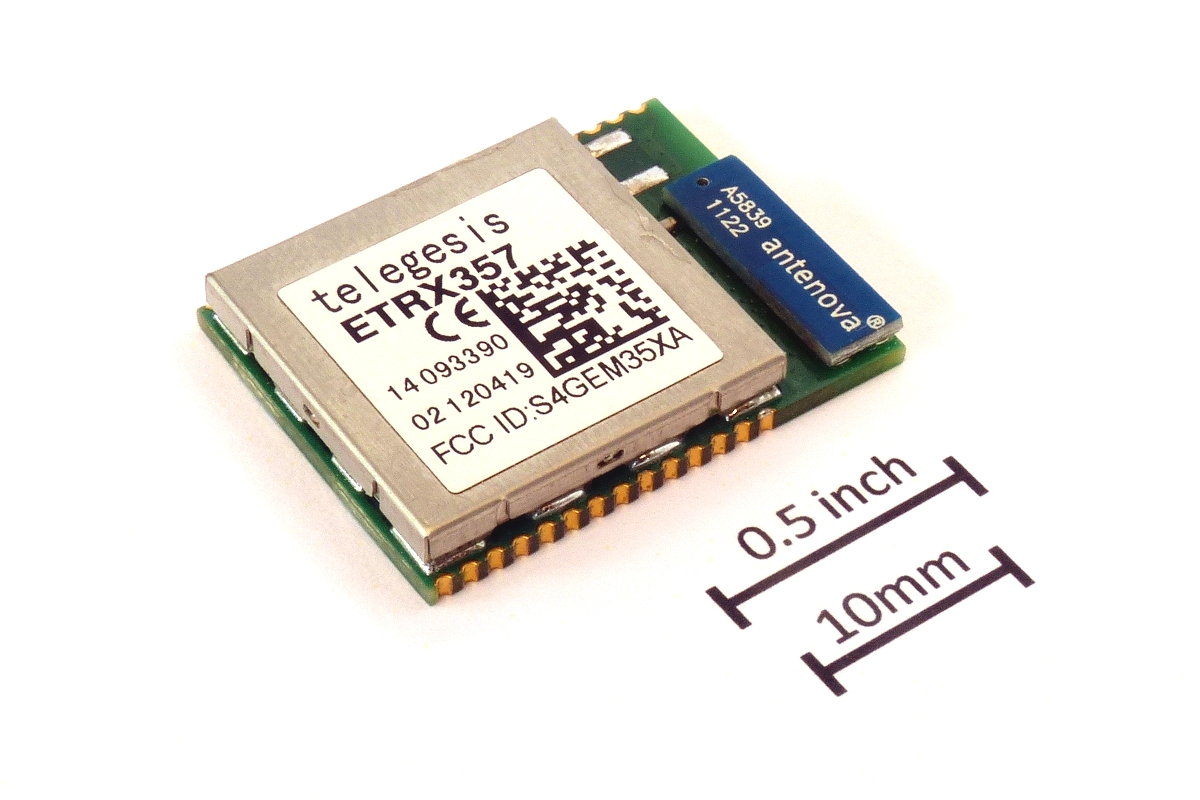
\includegraphics[height=2.5in]{figures/ETRX357_ZigBee_module_with_size_ref.jpg}
\caption[Modulo transductor de 2.4Gh Zigbee ETRX357]{Modulo transductor de Zigbee\footnotemark}
\end{figure}



\section{Hardware disponible}
\label{ch:Capitulo2.4}

Se han descrito algunas de las tecnologías características de las aplicaciones, topologías de red y protocolos de comunicación utilizados en domótica. Pero todo este entramado de software y señales deben operar en hardware físico. Más concretamente en múltiples dispositivos de hardware. En \gls{iot} el abanico de fabricantes de dispositivos orientados a sensorización y actuadores es tan extenso que simplemente está fuera de todo alcance el enumerarlos en este documento; aun así, considerando los objetivos definidos en el proyecto, que incluyen el uso de hardware open source, y costes de adquisición reducidos, podemos reducirlo a una lista de opciones acotada.

\vspace{1.5cm}

Es importante remarcar en este punto del documento, que en los proyectos de \gls{iot}, obtener el mejor balance de coste y eficiencia en la construcción es vital para soluciones profesionales. Para el prototipo que ocupa este proyecto, no se espera enfrentar este obstáculo, ya que no se encuentra definido en los objetivos el crear un sistema lo más equilibrado posible, sino uno funcional, respetando un límite de gasto que no supere la cuantía definida de 50 euros. Tampoco figura entre los objetivos asegurar un consumo energético los más reducido posible por parte de los dispositivos, pero se valorará la selección de equipamiento que, dando la mayor flexibilidad de configuración, se encuentre en valores de consumo lo suficientemente bajos como para que el prototipo sea fiable al ideal de una suite domótica funcional.

\vspace{1.5cm}

Partimos del concepto de suite domótica basado en dispositivos conectados a un nodo principal o \gls{gateway}, el cual actúa como router \gls{wifi}. Dicho \gls{gateway} posee un adaptador de red adicional que permite una conexión con la red de internet y que sea capaz de ejecutar servicios y aplicaciones actuando como servidor. Estos requisitos nos orientan a disponer de un ordenador completo, sera necesaria la flexibilidad de un SO que nos permita experimentar diferentes planteamientos, sin dejar de tener en cuenta que este ordenador tendrá una disponibilidad continua, y debe tener un consumo energético bajo y unos recursos suficientes para actuar como cimiento del prototipo.

\vspace{1.5cm}

Hace una década habría sido necesario apuntar a un equipo muy especializado y esto generalmente se traduce en un incremento del precio del equipo. Hoy, en cambio, disponemos de muchas opciones de ordenadores con un reducido factor de forma, bajo consumo eléctrico y recursos más que suficientes para cubrir muchos prototipos ligeros. Hablamos de la muy conocida Raspberry Pi y similares que has surgido con el tiempo (como Orange Pi, Banana Pi, Odroid o Matrix ARM ~\cite{lignuxComparative}), pueden encontrase en la figura \footnotetext{Comparativas de micro-ordenadores} algunos aspectos técnicos de sus capacidades comparadas entre sí.
. Para el caso que nos ocupa necesitamos que disponga de al menos dos adaptadores de red, uno de ellos inalámbrico, aunque puede subsanarse la falta del mismo mediante adaptadores inalámbricos USB (una estrategia muy común en los primeros modelos de Raspberry Pi hasta la serie 3). No es necesario que disponga de un procesador gráfico ya que operaremos de forma remota el ordenador mediante conexiones de SSH. Será un aspecto muy positivo que disponga de una interfaz para conectar dispositivos USB, este ultimo responde a la posible necesidad de conectar placas micro-controladoras para su programación.

\begin{figure}[hbt!]
\centering
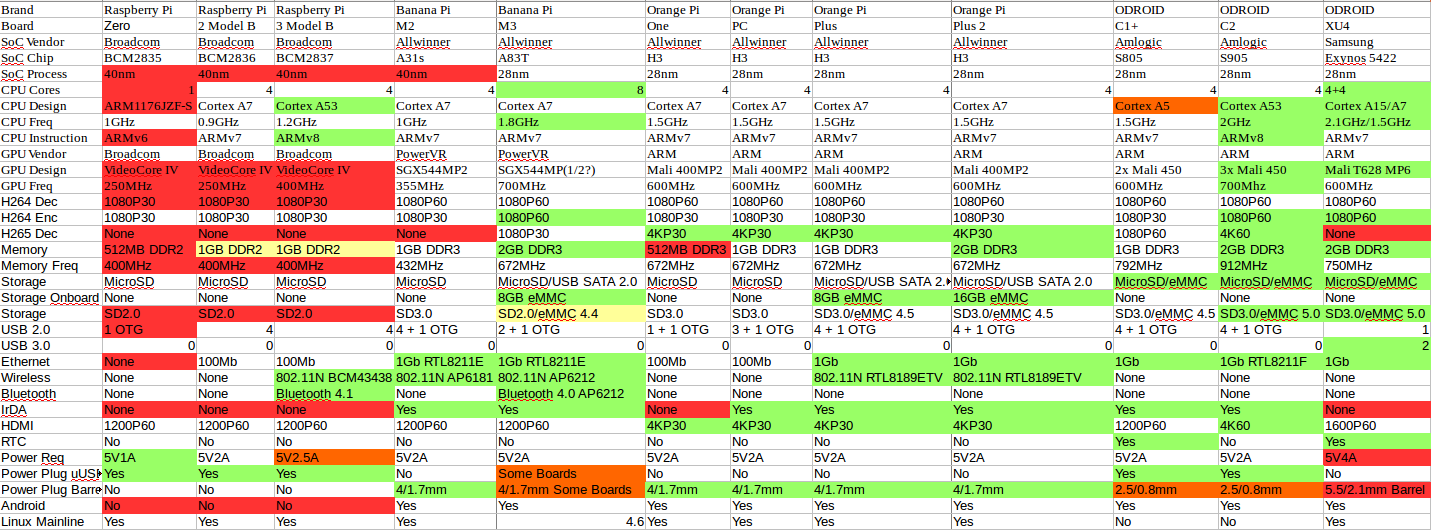
\includegraphics[height=2.5in]{figures/comparativaOrdenadores.png}
\caption[Comparativas de micro-ordenadores]{comparativa de características técnicas de micro-ordenadores\footnotemark}
\end{figure}


Raspberry Pi es posiblemente el uno de los mejores ejemplos de hardware abierto disponibles en el mercado. El diseño de su circuito impreso puede descargarse libremente para crear versiones modificadas.~\cite{raspberry_schematics}. Su precio puede variar notablemente dependiendo del vendedor, pero generalmente no debe superar los 35 euros. Dispone de capacidad suficiente para ejecutar distintos SO basados en arquitectura ARM. En el capítulo siguiente de la propuesta se evaluará que SO utilizar. De entre las distintas opciones disponibles, Raspberry Pi posee una de las comunidades de usuarios más grandes del mundo, posee una amigable documentación de uso e interminables ejemplos de uso y proyectos disponibles en la red. Sus especificaciones técnicas son suficientes para sostener los servicios necesarios para un prototipo de suite domótica, y puede alimentarse con una toma de USB de 5 Voltios.

\begin{figure}[hbt!]
\centering
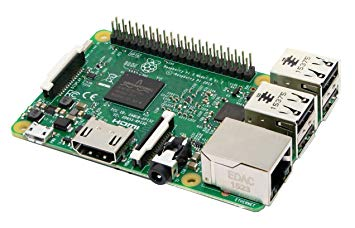
\includegraphics[height=2.5in]{figures/raspberrypi3b.jpg}
\caption[captura de una Raspberry]{Ordenador Raspberry Pi 3B\footnotemark}
\end{figure}

\vspace{1.5cm}


Esto cubriría el soporte físico necesario para crear un \gls{gateway}. Pero por sí solo no es suficiente. Los dispositivos que conectaremos a esta solución pueden presentarse en distintas opciones de hardware que pueden operar entre sí y con el propio \gls{gateway} mediante conectividad \gls{wifi}. Gracias a los protocolos de comunicación disponibles, un \gls{gateway} puede comunicarse con dispositivos de distintos fabricantes, presentando en la aplicación a todos ellos como dispositivos homogéneos con diferentes funciones.

\vspace{1.5cm}

En esencia, la clasificación de actores que conforman la red domótica se dividen en el \gls{gateway} (aunque pueden existir varios), los sensores y los actuadores. De hecho, un actuador no está restringido a actuar también como sensor y viceversa. Esta clasificación responde a la facilidad de entender rápidamente si un dispositivo actúa como entrada o salida del sistema. En \gls{iot} es habitual disponer de hardware especializado de bajo consumo y orientado a protocolo concretos de comunicación para ser usados en \gls{framework}, como ocurre con OpenHab, que facilita bastante la tarea de incluir nuevos dispositivos a la suite domótica si el producto a integrar ya está implementado. Si se desea disponer de la flexibilidad de cambiar radicalmente el comportamiento de un actor, modificando su comportamiento y hardware, es mejor plantear el uso de placas microcontroladoras programables.

\vspace{1.5cm}

Estas placas, al no estar sujetos a un implementación y diseño cerrados, pueden cambiar y ajustarse a nuevos comportamientos y especificaciones, lo cual aportan mayor escalabilidad y facilita la capacidad de actualizar el código programado. Por contrapartida, al ser de uso genérico, su consumo eléctrico para operar es mayor que en los dispositivos diseñados específicamente para una tarea concreta. Es sin embargo, una limitación aceptable, ya que el prototipo busca la funcionalidad sobre el rendimiento.

\vspace{1.5cm}

Uno de los ejemplos mas conocidos y amigables de usar en placas micro-controladoras programables es Arduino. Estas placas disponen de conexiones \gls{io} que pueden usarse para ampliar su abanico e capacidades técnicas, en prototipos de \gls{iot}, es habitual dotar a una placa con conectividad \gls{wifi} mediante un adaptador inalámbrico conocido como shield.

\vspace{1.5cm}

En los últimos años ha aparecido un pequeño microcontrolador con chip de \gls{wifi} conocido generalmente como modulo ESP-01. Este chip permite una comunicación con el protocolo TCP/IP en una red inalámbrica. Se clasifica como hardware RF/IF y RFID CI de transceptor RF, capaz de operar con el protocolo 802.11b/g/n de 2.4GHz. El modelo ESP8266 que actualmente se comercializa posee capacidades superiores a su predecesora ESP8265 incluye una mayor capacidad de memoria flash interna, suficiente para abordar la mayoría de dispositivos \gls{iot} que pretendan actuar como actuadores o sensores.
Sin embargo, trabajar y programar estos chips puede resultar engorroso si no se dispone de USB con interfaz para escritura en serie, también puede hacerse con una placa de Arduino separando la cucaracha del microcontrolador del Arduino y cableando la conexión necesaria para programarse desde un ordenador.

\begin{figure}[hbt!]
\centering
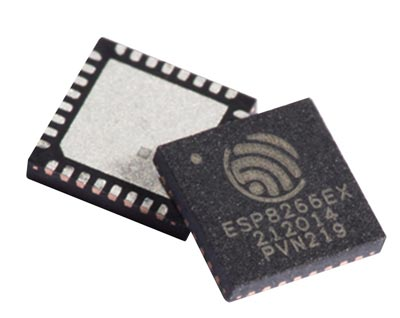
\includegraphics[height=2.5in]{figures/esp8266ex.jpg}
\caption[controladora ESP8233]{controladora ESP8266\footnotemark}
\end{figure}

\vspace{1.5cm}

Este microcontrolador opera con apenas 3.3VDC, lo cual es considerado como una ventaja a la hora de incluir este modulo en proyectos que operan sobre otras placas micro-controladoras como Arduino. Sin embargo, esta opción es válida sólo para la creación de prototipos funcionales, ya que el modulo ESP-01 requiere de un amperaje de al menos 200mAh para operar con normalidad. Los pines de alimentación de 3,3V de placas como Arduino ofrecen unos 50mAh de intensidad de corriente. Esto es suficiente para que el modulo opere, pero ocasionalmente puede causar daños en el modulo y generalmente el funcionamiento de la conexión es de baja calidad, con poca intensidad de señal, perdidas de paquetes y caídas de la conexión. La estrategia más extendida en facilitar una conexión estable de alimentación al modulo separado de la alimentación recibida por la placa microcontroladora en la que opera.

\vspace{1.5cm}

También pueden ejecutarse construcciones simples en una breadboard para un divisor de potencia mediante resistencias que transforme la señal de 5V de las placas microcontroladores, que habitualmente ofrecen un mayor valor de amperios, para dar una señal de 3.3VDC con mas de 200mA. Siendo realistas, no es ni siquiera necesario crearlos si se considera las opciones de venta de algunos fabricantes que montan una microcontrolador con chip ESP8266 en una ensamblada con las resistencias necesarias, interruptores y habitualmente sensores o actuadores como el mostrado en la imagen siguiente\footnotetext{ESP-01S con relé} a modo de módulo compacto alimentado por pines a 5V. El precio de estos módulos apenas alcanza un par de euros si se solicita a vendedores chinos, pero, es conveniente entender los riesgos que se asume al adquirir estos dispositivos de fabricantes clónicos con dudosos controles de calidad, que pueden seleccionar componentes incompatibles son redes \gls{wifi} como el suministrado por el adaptador inalámbrico de una Raspberry Pi 3B. Más información sobre estos problemas están ampliados en anexo B de troubleshooting.

\begin{figure}[hbt!]
\centering
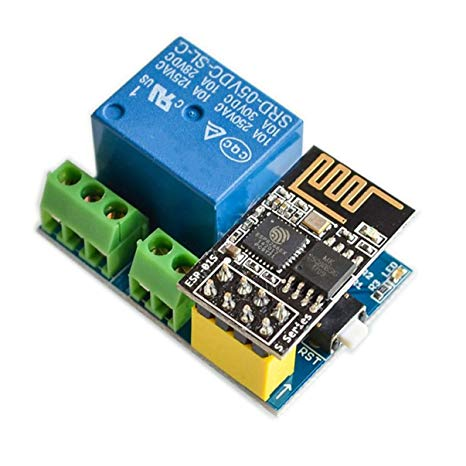
\includegraphics[height=2.5in]{figures/esp8266exRele.jpg}
\caption[ESP-01S con rele]{ESP8266 5V Modulo Rele\footnotemark}
\end{figure}

\vspace{1.5cm}

Con las complicaciones de alimentación del modulo ESP8266 surge al poco tiempo su sucesor natural, las placas nodeMCU. Conocidas por ser plataformas de código abierto para \gls{iot} más versátiles y accesibles en coste de adquisición. Uno de los aspectos que popularizó estos dispositivos fue la posterior portabilidad de la biblioteca de \gls{mqtt}, permitiendo al LUA de la SOC desplegar dicho protocolo. Aunque el proyecto de mantenimiento de firmware fue abandonado en 2015 por los autores originales, la comunidad de usuarios siguió mejorando el código hasta fecha de hoy, convirtiendo el nodeMCU en uno de los dispositivos mas demandados en proyectos, gracias a su bajo coste de precio, inferior a una decena de euros por placa, que dispone de 12 pines de GPIO permitiendo implementaciones complejas que aprovechan la conectividad inalámbricas para proyectos de \gls{iot}

\begin{figure}[hbt!]
\centering
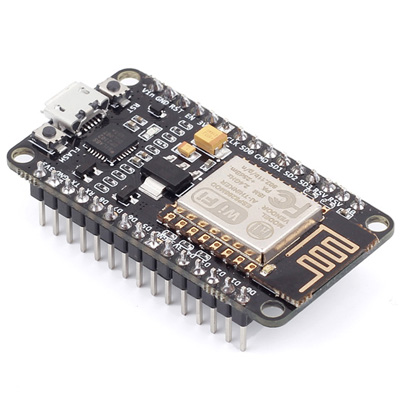
\includegraphics[height=2.5in]{figures/nodemcu.jpg}
\caption[captura de una nodeMCU]{Microcontroladora NodeMCU\footnotemark}
\end{figure}
\cleardoublepage

\chapter{Propuesta}
\label{ch:Capitulo3}

Tras presentar diferentes tecnologias, software, protocolos de comunicación y hardware planteados en el ámbito de la domótica del hogar, en la búsqueda de una solución libre y de bajo coste, que pueda alcanzar los objetivos planteados para la creación de un prototipo de suite domótica, se propone:

Desarrollar un prototipo de suite domótica que opere en una red local inalámbrica cuyo router actúe como nodo principal, ejecutado en un ordenador de bajo consumo, que permita la interconexión para dispositivos inalámbricos con roles de actuadores o sensores. Además, debe ser posible operar dicha suite, desde dentro de la red local, o desde fuera de la misma mediante conexiones remotas, por una aplicación para dispositivo movil con sistema operativo Android. Si bien, la operatividad remota es opcional, se debe alcanzar la gestión de la suite en el entorno de la red local, cumpliendo asi con el objetivo de disponer de un sistema aislado y autónomo, que no dependa de servicios externos para su funcionamiento.

Adicionalmente se tratará de alcanzar una cierta descentralización de los dispositivos y la propia raspberry, basándose en el concepto de nodo principal (gateway), que habitualmente se observa en las plataformas de pago.

Para lograr dicha propuesta, será necesario considerar de entre las opciones estudiadas aquellas que se ajustan mejor al alcance de esta propuesta. Dadas las distintas capas de hardware, arquitectura de red y software que componen este proyecto, la propuesta será dividida en tres conceptos modulares, permitiendo un desarrollo individual y en paralelo respecto de cada uno.

Habiendo elegido no utilizar un framework concreto, queda a nuestra entera disposición seleccionar bajo que servicios operara nuestra solución domótica. Cualquiera de los frameworks anteriormente listados estaban sujetos a una combinación de servicios que les permitía operar dentro de sus especificaciones. En más de la mitad de ellos, se utilizaban servidores web que permitan gestionar la suite domótica vía web, o a través de una app.

Una vez alcanzada una implementación funcional del prototipo se aplicará en dos casos de usos que ejemplifican la entrada y salidas características de todo sistema de domótica, la recepción, proceso y presentación de datos de un dispositivo sensor en la aplicación movil, y la gestión de un actuador desde dicha aplicación.

Dichos planteamientos se basan en que todo sensor/actuador que forme parte de red de dispositivos de una solución de domótica actual, es gestionada a través de un nodo. En vez de conectar los dispositivos inalámbricos a el router de la casa, se conectan al nodo y este, a su vez, es quien se conecta a la red local del hogar, para asi conectarse con los servicios externos. En general, las distintas plataformas has alcanzado un acuerdo no formalizado de actuación que funciona de la siguiente forma. El usuario final compra un nuevo dispositivo, lo enciende, dejándolo en un estado de "inclusión" a la red domótica, después, desde la aplicación de movil, se indica al nodo, que se quiere añadir un nuevo dispositivo, y tras seguir las indicaciones, el dispositivo se registra en la red del nodo. Esto, sin embargo, tiene algunos inconvenientes en el proceso de "inclusión", y aunque la probabilidad es baja, puede suceder que dos nodos de distintas viviendas, que están registrando dispositivos simultáneamente, terminasen, registrando un dispositivo que no les corresponde. Esto es una vulnerabilidad de seguridad grave y una vertiente adicional que incluir en las motivaciones del estudio y desarrollo de una suite domótica libre que permita nuevas formulas de funcionamiento.

Se ha planteado este problema, junto con las 3 motivaciones principales, para crear un proceso de "inclusión" de dispositivos al nodo, que parta de una conexión alámbrica (vía USB) y resuelva este inconveniente, y simplifique el proceso de las soluciones privadas, que en ocasiones pueden fallar.

Podría parecer que hablamos de una relación de objetos entre sí, y que un modelo de BBDD relacional es la mejor opción, pero si consideramos que, cada entrada almacenada tendrá una estructura distinta, hace que no sea una opción tan ideal. Pensemos, por ejemplo, que utilizando una BBDD SQL se planifica un conjunto de tablas relacionadas entre sí. Sera necesaria una tabla que contenga las ubicaciones y se relacione con otra tabla que definan a los dispositivos. Esto establece una relación 1:N donde múltiples dispositivos pueden existir para una estancia, pero nunca en varias a la vez. De cada dispositivo existirá una nueva relación 1:N de medidas. Lo cual deja un esquema semejante al de la figura siguiente:


\begin{figure}[hbt!]
\centering
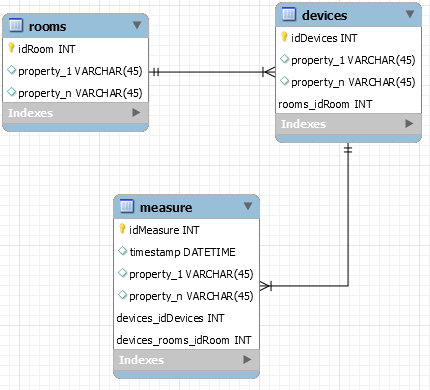
\includegraphics[height=2.5in]{figures/SQLSchemaExample_1.png}
\end{figure}

\vspace{1.5cm}

Sin embargo, existen algunos problemas graves de diseño de esta idea, en primer lugar, los dispositivos no pueden ser una propiedad de una estancia. Son objetos relacionados, pero no existe una transitividad dura entre ellos. Un dispositivo puede cambiar de estancia en un momento dado, y aun asi, seguir existiendo medidas en fechas concretas de ese dispositivo para una habitación en la cual, dicho dispositivo ya no está relacionado. Otro posible escenario es la desaparición de una estancia (como resultado de fusionar 2 estancias en una al derribar una pared). Para mantener una integridad lógica y persistente a lo largo del tiempo. Toda medida deberá tener un campo que determine en que ubicación fue tomada.
no hay transitividad dura entre room y device, lo cual hace que sean independientes entre sí.


\begin{figure}[hbt!]
\centering
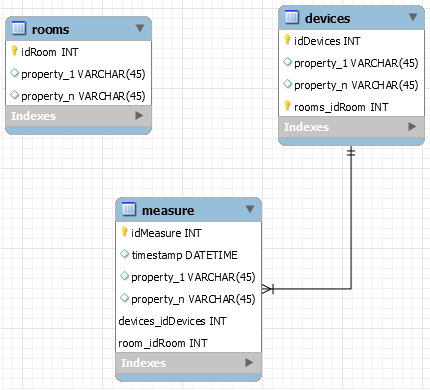
\includegraphics[height=2.5in]{figures/SQLSchemaExample_2.png}
\end{figure}

\vspace{1.5cm}

Con esto aún tendríamos que enfrentar un problema adicional, el número de columnas que definen las propiedades de una tabla. El ejemplo más claro es la tabla de medidas. Una medida, efectuada por un sensor será definida por su identificador y la fecha en la que se realizó, ahora bien, según la naturaleza del dispositivo, se obtendrán disantos tiempos de medida. Un sensor combinado de temperatura y humedad nos dará dos magnitudes de medición, un sensor de ruido almacenará un valor de decibelios, una luz define su medida por su estado de actividad (encendido o apagado), aunque por otra parte podría indicar el consumo eléctrico, o propiedades adicionales como intensidad de luz, o incluso color. Es cierto que, para un actuador, como lo es un emisor de luz, no realiza medidas como tal, y sus correspondientes estados de actividad podrían ser más adecuados definirlos como propiedades del dispositivo y no como medidas. Podríamos separar las medidas de los estados en tablas distintas, pero igualmente llegaríamos al problema del número de campos necesarios en una tabla. Valor que por otra parte es muy difícil de prever en base a la extensa gama de dispositivos existentes. Esto puede solucionarse de manera sencilla con 2 estrategias. Incluir una gran cantidad de columnas en previsión de los distritos tipos de medidas existentes, dejando que las medidas posean un valor nulo para los campos no utilizados en función de la relación de su sensor, o bien, unificar todos los campos en un único valor de cadena de caracteres que almacene un dato estructurado, como es el caso de los JSON. Esta última opción, sería la más deseable tanto por sencillez de implementación como facilidad de procesamiento. Lo que dejaría un esquema semejante a este:

\begin{figure}[hbt!]
\centering
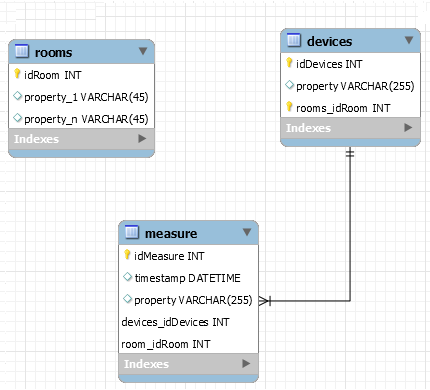
\includegraphics[height=2.5in]{figures/SQLSchemaExample_3.png}
\end{figure}

Una preocupación que agrava la perspectiva de usar una BBDD relacional es, en este punto del proyecto, su escalabilidad horizontal. Si bien las tablas pueden crecer a un gran número de registros, no se prevé almacenar datos con vistas a largo plazo, la mayoría de los valores almacenados serán efímeros en tiempo de utilidad, almacenarlos responde solo a la necesidad de obtener comparativas en plazos de tiempo relativamente cortos, como horas, dias, y posiblemente semanas. Mas alla de este rango estos datos no tienen una utilidad real y pueden ser condensados en médias para utilizarse en resúmenes. Por otro lado, disponer de flexibilidad a la hora de configurar la extensión de propiedades de un objeto de la BBDD es uno de los puntos fuertes de una BBDD no relacional.

\vspace{1.5cm}


\section{Módulos de la propuesta}
\label{ch:Capitulo3.2}

Se creará un nodo principal que actuara como router de la red de dispositivos de la suite domótica y servidor de la aplicación movil. Dispondrá de la capacidad de ser operado de forma remota o local, almacenara los servicios y aplicaciones necesarios para que funcione la suite domótica ejecutándose en un ordenador de bajo consumo.

Se genera distintos dispositivos sensores o actuadores que podrán incluirse en la red inalámbrica del nodo principal y podrán ser operados desde dicho nodo.

Y por último la aplicación movil (front-end) y servidor (back-end) que darán al usuario la capacidad de gestionar la suite domótica.

\section{Propuesta de casos de uso}
\label{ch:Capitulo3.3}

El primer caso de uso consistirá en una simple interacción del usuario con la suite domótica para consultar la temperatura y/o humedad de una estancia. Para ello, es necesario disponer de un dispositivo inalámbrico con un sensor que recoja las mediciones y puedan ser mostradas al usuario en su smartphone.

El segundo caso de uso cubrirá la gestión por parte del usuario de un actuador basado en un interruptor de corriente, pudiendo consultar su estado actual y alternar dicho estado, también desde un smartphone.

\section{Objetivos adicionales}
\label{ch:Capitulo3.4}

Las siguientes propuestas corresponden más a un declaración de intenciones que a objetivos necesarios para cumplir la propuesta del proyecto. Son un valor añadido y deseable siempre que no comprometan los plazos de tiempo marcados por la entrega final de este documento al director de proyecto. Se encuentran enumerados según el valor de importancia.

\begin{enumerate}

  \item Vinculación de dispositivos con la red de suite domótica mediante USB, en lugar del clásico emparejamiento WIFI.

  \item Creación de una imagen autoinstalable de para otros usuarios

  \item Integración de múltiples opciones de hardware compatibles con la suite domótica.

  \item Conexiones cifradas en la red de dispositivos y en la comunicación entre aplicación movil y servidor.

  \item Exportar la suite domótica en una imagen autoinstalable, de fácil instalación que permita replicar el prototipo creado.

\end{enumerate}

\begin{figure}[hbt!]
\centering
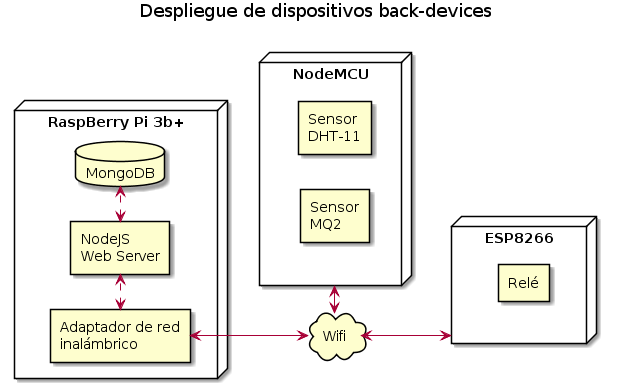
\includegraphics[height=2.5in]{figures/diagrams/physical-devices/back-devices.png}
\caption[back-devices]{back-devices\footnotemark}
\end{figure}
\cleardoublepage

\chapter{Arquitectura e Implementación}
\label{makereference4}

\section{Equipamiento}
\label{makereference4.1}

Existen múltiples niveles de implementación del prototipo planteado en este documento. En función de la cantidad de módulos operativos se requerirá una mayor cantidad de hardware para la sensorización y los actuadores implicados. El nivel más básico e imprescindible implica un ordenador con SO Linux que actuará como controlador de la infraestructura de dispositivos que dan forma al sistema en su conjunto, esto será referido en adelante como el nodo principal.

\section{Definición del nodo principal}
\label{makereference4.2}

El nodo principal representa el núcleo de una suite domótica. Los sensores y actuadores dispuestos en un hogar lo usan como centro neurálgico para que el sistema opere, y la aplicación móvil lo usa como servidor para obtener la información registrada por esos dispositivos e interactuar con ellos. Si bien los sensores son capaces de registrar datos por su cuenta, estos deben ser entregados en el \gls{gateway} para ser procesados de forma útil respeto al resto de la infraestructura. 

\vspace{1cm}

Como soporte de hardware, se usará un ordenador compacto de la marca Raspberry Pi. La selección particular de este dispositivo se apoya en dos características esenciales en el desarrollo de este proyecto: es barato, de bajo consumo eléctrico y aunque no está clasificado como \verb|Open Hardware| ya que la Raspberry Pi Foundation requiere de los ingresos de las ventas de sus distintos modelos de Raspberry, su proyecto goza de buena reputación en el mundo educativo y se considera una organización benéfica con el objetivo de acercar la electrónica a todo el mundo. Además, goza de una gran presencia en el mercado de electrónica, por lo cual es fácil de adquirir y ha acumulado una extensa comunidad de usuarios que muestran su uso mediante tutoriales y experimentos. Como motivos adicionales se encuentra su reducido tamaño que permite ubicarlo con facilidad en lugares estrechos o difícilmente accesibles, además de su imperceptible ruido al operar. El modelo concreto para el desarrollo del prototipo es Rapsberry Pi3b+ que dispone de capacidad de procesador y memoria RAM suficiente para operar todo el software necesario. Este modelo no integra un almacenamiento interno para el usuario, pero su interfaz incluye una ranura de tarjetas micro-SD compatible con prácticamente todas las opciones de tamaño de almacenamiento disponibles en el mercado. Se precisan de al menos 4 \gls{gb} de espacio disponible en la memoria del sistema, y es recomendable exceder este mínimo siempre que sea posible, ya que la acumulación de datos con el paso del tiempo por parte del dispositivo puede crecer indefinidamente.

\vspace{1cm}

El nodo principal ejecuta Raspbian. Un \gls{so} \verb|GNU/Linux| diseñado específicamente para la arquitectura ARMv7 de los distintos modelos de ordenadores Raspberry. Concretamente, en este proyecto se utiliza la serie de distribuciones \verb|Lite|, orientadas a la ejecución del sistema operativa mediante interfaz de linea de comandos en terminal. Esta decisión está fundamentada en desprenderse de la necesidad de periféricos externos e interfaces de \verb|I/O| analógicas para controlar el \gls{so}. Toda configuración del sistema será realizada mediante conexiones por \gls{ssh}. El proceso de instalación y configuración de conexiones esta ampliado en el apéndice~\ref{AppendiA:Key2} del documento.

\vspace{1cm}

Una vez establecidos los medios de comunicación, se instalarán aplicaciones que permitirán ejecutar los servicios necesarios para actuar como nodo central. La estrategia de comunicación entre los distintos dispositivos que conforman la suite domótica se basa en un servidor \verb|NodeJs| que establece conexiones vía \gls{wifi} con los sensores y actuadores mediante el protocolo \gls{mqtt}, y este a su vez con la aplicación móvil vía \gls{wifi} o internet, mediante el protocolo \gls{https}. Se realizara una descripción mas concisa del software necesario en el nodo principal en el apartado \ref{makereference4.3}.



\begin{figure}[hbt!]
\centering
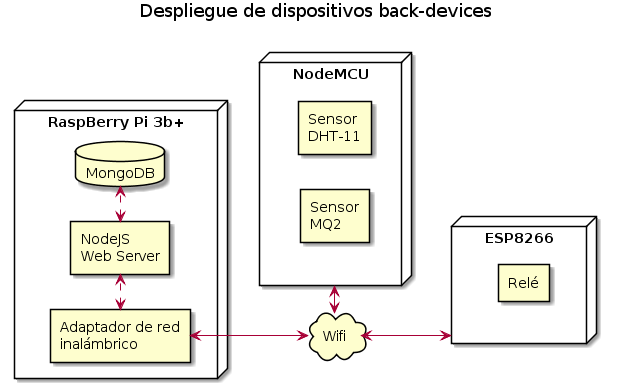
\includegraphics[height=2.5in]{figures/diagrams/physical-devices/back-devices.png}
\caption[Diagrama de despliegue de back-end]{Diagrama de despliegue de dispositivos y gateway\footnotemark}
\end{figure}

\section{Criterio de selección de dispositivos y Software}
\label{makereference4.3}

\begin{figure}[hbt!]
\centering
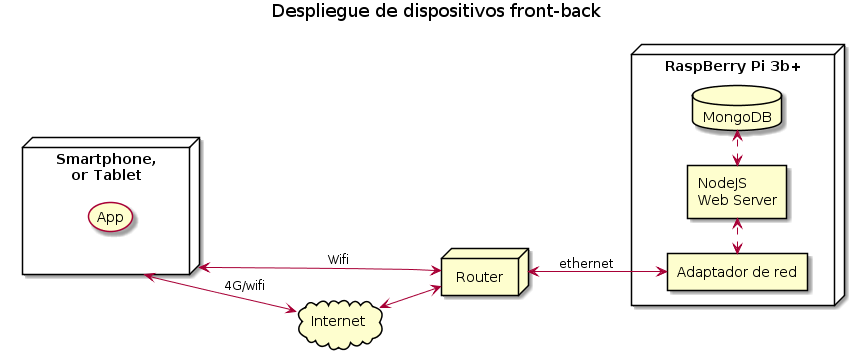
\includegraphics[height=2.5in]{figures/diagrams/physical-devices/front-back.png}
\caption[Despligue de front]{Diagrama de despliegue de smartphone, router y gateway\footnotemark}
\end{figure}

\section{Criterio de selección servicios}
\label{makereference4.4}
La selección de un servicio para la gestión de la \gls{bbdd}


Podría parecer que hablamos de una relación de objetos entre sí, y que un modelo de \gls{bbdd} relacional es la mejor opción, pero si consideramos que, cada entrada almacenada tendrá una estructura distinta, hace que no sea una opción tan ideal. Pensemos, por ejemplo, que utilizando una \gls{bbdd} SQL se planifica un conjunto de tablas relacionadas entre sí. Sera necesaria una tabla que contenga las ubicaciones y se relacione con otra tabla que definan a los dispositivos. Esto establece una relación 1:N donde múltiples dispositivos pueden existir para una estancia, pero nunca en varias a la vez. De cada dispositivo existirá una nueva relación 1:N de medidas. Lo cual deja un esquema semejante al de la figura siguiente:


\begin{figure}[hbt!]
\centering
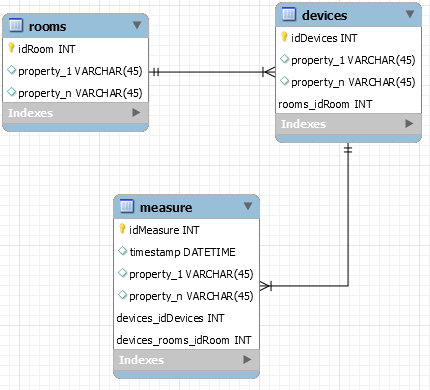
\includegraphics[height=2.5in]{figures/SQLSchemaExample_1.png}
\caption[Primer planteamiento de diseño de BBDD relacional]{Primer planteamiento de diseño de BBDD relacional\footnotemark}
\end{figure}

\vspace{1.5cm}

Sin embargo, existen algunos problemas graves de diseño de esta idea, en primer lugar, los dispositivos no pueden ser una propiedad de una estancia. Son objetos relacionados, pero no existe una transitividad dura entre ellos. Un dispositivo puede cambiar de estancia en un momento dado, y aun asi, seguir existiendo medidas en fechas concretas de ese dispositivo para una habitación en la cual, dicho dispositivo ya no está relacionado. Otro posible escenario es la desaparición de una estancia (como resultado de fusionar 2 estancias en una al derribar una pared). Para mantener una integridad lógica y persistente a lo largo del tiempo. Toda medida deberá tener un campo que determine en que ubicación fue tomada.
no hay transitividad dura entre room y device, lo cual hace que sean independientes entre sí.


\begin{figure}[hbt!]
\centering
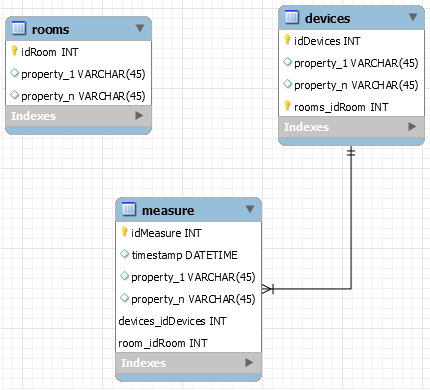
\includegraphics[height=2.5in]{figures/SQLSchemaExample_2.png}
\caption[Segundo planteamiento de diseño de BBDD relacional]{Primer planteamiento de diseño de BBDD relacional\footnotemark}
\end{figure}

\vspace{1.5cm}

Con esto aún tendríamos que enfrentar un problema adicional, el número de columnas que definen las propiedades de una tabla. El ejemplo más claro es la tabla de medidas. Una medida, efectuada por un sensor será definida por su identificador y la fecha en la que se realizó, ahora bien, según la naturaleza del dispositivo, se obtendrán disantos tiempos de medida. Un sensor combinado de temperatura y humedad nos dará dos magnitudes de medición, un sensor de ruido almacenará un valor de decibelios, una luz define su medida por su estado de actividad (encendido o apagado), aunque por otra parte podría indicar el consumo eléctrico, o propiedades adicionales como intensidad de luz, o incluso color. Es cierto que, para un actuador, como lo es un emisor de luz, no realiza medidas como tal, y sus correspondientes estados de actividad podrían ser más adecuados definirlos como propiedades del dispositivo y no como medidas. Podríamos separar las medidas de los estados en tablas distintas, pero igualmente llegaríamos al problema del número de campos necesarios en una tabla. Valor que por otra parte es muy difícil de prever en base a la extensa gama de dispositivos existentes. Esto puede solucionarse de manera sencilla con 2 estrategias. Incluir una gran cantidad de columnas en previsión de los distritos tipos de medidas existentes, dejando que las medidas posean un valor nulo para los campos no utilizados en función de la relación de su sensor, o bien, unificar todos los campos en un único valor de cadena de caracteres que almacene un dato estructurado, como es el caso de los JSON. Esta última opción, sería la más deseable tanto por sencillez de implementación como facilidad de procesamiento. Lo que dejaría un esquema semejante a este:

\begin{figure}[hbt!]
\centering
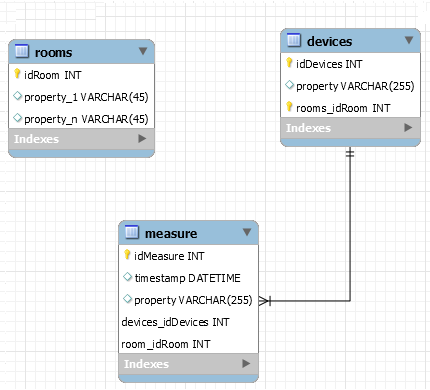
\includegraphics[height=2.5in]{figures/SQLSchemaExample_3.png}
\caption[Tercer planteamiento de diseño de BBDD relacional]{Primer planteamiento de diseño de BBDD relacional\footnotemark}
\end{figure}

Una preocupación que agrava la perspectiva de usar una \gls{bbdd} relacional es, en este punto del proyecto, su escalabilidad horizontal. Si bien las tablas pueden crecer a un gran número de registros, no se prevé almacenar datos con vistas a largo plazo, la mayoría de los valores almacenados serán efímeros en tiempo de utilidad, almacenarlos responde solo a la necesidad de obtener comparativas en plazos de tiempo relativamente cortos, como horas, días, y posiblemente semanas. Mas allá de este rango estos datos no tienen una utilidad real y pueden ser condensados en medias para utilizarse en resúmenes. Por otro lado, disponer de flexibilidad a la hora de configurar la extensión de propiedades de un objeto de la \gls{bbdd} es uno de los puntos fuertes de una \gls{bbdd} no relacional.


\section{Arquitectura de la aplicación frontend}
\label{makereference4.5}

\subsection{Consideraciones previas}
\label{makereference4.5.1}

El desarrollo de la app frontend se ha servido de dos frameworks para salvar ciertos escollos básicos no relacionados con la implementación de la suite domótica. Por un lado, se ha hecho uso del framework Open Source Ionic (en su versión 3), que es un framework Open Source para la construcción de aplicaciones híbridas multiplataforma, que nos permitirá portar la aplicación para cualquier dispositivo móvil Android a través de Cordova, y que además nos permitirá hacer uso de capacidades nativas de los dispositivos móviles (como el módulo de Wifi) gracias a los plugins existentes para ello. Además, Ionic proporciona grandes herramientas en cuanto a la maquetación responsive, lo cual ayuda en la creación de una aplicación móvil sin necesidad de invertir grandes esfuerzos en alcanzar un aspecto, usabilidad y elegancia mínimos y pudiendo redirigir ese esfuerzo a otros terrenos más fructíferos. Ionic está basado en Angular, el otro framework del que se ha hecho uso (en su versión 5) especialmente por su enfoque en una arquitectura basada en componentes que puedan ser reutilizados con mucha facilidad a lo largo de toda la aplicación. Las versiones modernas de Angular hacen uso de TypeScript para la programación de su lógica de negocio, lo que permite una mayor limpieza de código, mejores herramientas de tipado estricto y redunda en mayor escalabilidad. Angular se programa en TypeScript para la lógica de negocio, SASS para los estilos css y HTML para la maquetación.

\vspace{0.5cm}

\subsection{Estructura básica}
\label{makereference4.5.2}

A grandes rasgos, la aplicación frontend está estructurada en:
\begin{enumerate}
 \item Componentes, por lo general tendremos casi tantos como trozos o segmentos en los que se quiera desestructurar una vista (los conoceremos como \textit{component}; serán útiles para aislar los diferentes comportamientos que se puede requerir en cada vista, y un mismo componente puede ser replicado infinitamente a lo largo de la aplicación cada vez con unos parámetros diferentes.
 \item Módulos de vistas, generalmente uno por cada vista de la aplicación (lo que conoceremos como \textit{view} o \textit{template}); se encargarán de cargar la información que requiere la vista y de transformar las interacciones del usuario con la vista en flujos lógicos que generalmente pasan por (o acaban en) otros módulos.
 \item Centros de gestión y manipulación de datos, generalmente uno por cada estructura de datos existente (lo que conoceremos como \textit{store}); su cometido será proporcionar métodos a otros módulos o vistas para obtención y/o manipulación de su tipo de datos, siendo la store la responsable última de obtenerlos, manipularlos o almacenarlos por cualquier medio existente.
 \item Servicios que ejercerán de cómodas APIs contra APIs externas o contra \gls{bbdd} locales del dispositivo (los que conoceremos como \textit{api provider/service} en el primer caso y \textit{database service} en el segundo), generalmente uno de cada por cada estructura de datos existente; son responsables de lanzar las llamadas a dichos servicios con los parámetros adecuados (bien seas APIs REST remotas o \gls{bbdd} locales) y controlar sus respuestas.
 \item Servicios, que implementan utilidades y herramientas a lo largo de toda la aplicación de forma independiente, tanto que, técnicamente, podrían formar parte de cualquier otra aplicación (los que conoceremos como \textit{service}); son responsables de aportar utilidades puntuales con la suficiente abstracción como para que el "usuario" de dicho servicio no conozca su funcionamiento en detalle, sino más bien, le resulte sencillo, conveniente y cómodo acudir a sus métodos.
\end{enumerate}

\vspace{0.5cm}

Con el fin de comprender el esquema utilizado, mencionaremos los tipos de estructura existentes, aun cuando detallaremos su flujo más adelante: tendremos los dispositivos, que serán conocidos como \textit{things} (siendo posiblemente lo más adecuado debido a su famosa acepción en el \gls{iot}); las habitaciones, que mencionaremos aquí y allá como \textit{rooms}; los usuarios, que conoceremos como \textit{users}; las placas, que mencionaremos como \textit{boards}; y los datos de aplicación generales, a los que nos referiremos como \textit{application data}. Se observará que, en todos los casos, nos conviene referirlos en su traducción al inglés por facilidad a la hora de seguir el hilo del flujo en el código.

\subsection{Patrón del flujo de datos}
\label{makereference4.5.3}

En pro de aplicar una arquitectura que intenta aplicar los principios de separación de responsabilidades y capas de abstracción, a continuación explicamos los patrones que sigue la estructura del proyecto frontend.

\begin{figure}[hbt!]
\centering
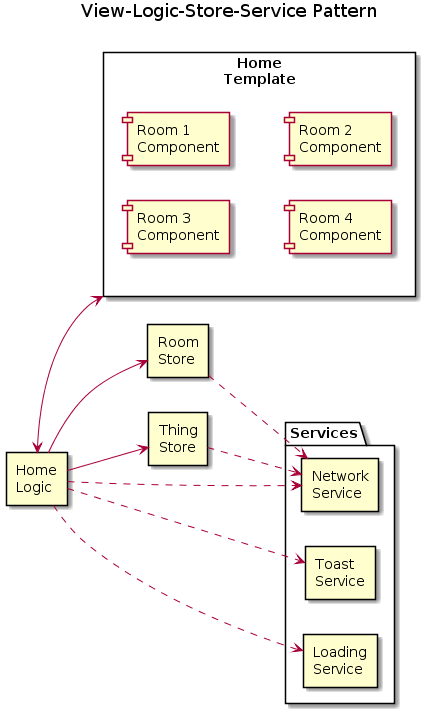
\includegraphics[height=5in]{figures/diagrams/front/architecture/view-logic-store-service-pattern.png}
\caption[view-logic-store-service-pattern]{View-Logic-Store-Service Pattern\footnotemark}
\label{fig:front-view-store}
\end{figure}

\vspace{0.5cm}

Por lo general, todas las vistas presentan, bajo un formato u otro, una serie de datos. El template será por tanto responsable de adaptar y mostrar estos datos como se requiera; pero primero deben obtenerlos, para lo cual delegarán en la store. A partir del momento en que se pide estos datos a la store, se crea una conveniente capa de abstracción que es útil en dos sentidos principales: por un lado, la vista no debe preocuparse del origen de dónde obtener esos datos, esto será responsabilidad de la store, lo cual hace más limpio el código del template, que debe preocuparse estrictamente de atender a los requisitos y cambios de la vista; por otro, la misma lógica que deba implementar la store para ofrecer estos datos a una vista, podrá ser reaprovechada para ofrecérselo a otra. 

\vspace{0.5cm}

En el ejemplo de la Figura \ref{fig:front-view-store}, podemos observar como el template de la vista \textit{Home} debe mostrar una lista de todas las habitaciones existentes. Una vez el template ha adquirido este array de rooms a partir de la room store, deberemos mostrar un componente room por cada room en esa lista. Sin embargo, la longitud de esta lista no es conocida de antemano, y puede cambiar en cualquier momento. Por tanto, la implementación debe ajustarse a este dinamismo. Angular nos permite, mediante su directiva \textit{ngFor}, generar tantos elementos como existan en un array de la lógica asociada al template, y además pueden ser elementos de cualquier tipo, luego esto nos sirve para crear una lista de componentes room, siendo posible instanciar cada uno con la información específica de cada elemento del array.

\vspace{0.5cm}

Observaremos que tanto la lógica asociada a una vista como las stores (así como otros services) hacen uso de los services. Estos services ofrecen, de forma autónoma e independiente, ciertas utilidades, como por ejemplo el LoadingService, que ofrece un spinner de carga con un mensaje de feedback para el usuario de que un proceso está cargando. El encargado de poseer y ejecutar la lógica que crea y muestra el spinner será el LoadingService; sin embargo, quien manda la orden inicial será siempre quien invoca al servicio, pues es quien conoce el estado actual de la vista: si los datos han sido pedidos y está a la espera de recibirlos, pedirá mostrar el spinner; si finalmente se recibe confirmación de que la vista ya tiene disponibles los datos, se ordenará ocultar el spinner. 

\vspace{1cm}

\begin{figure}[hbt!]
\centering
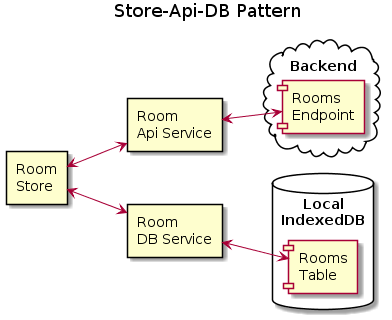
\includegraphics[height=2.5in]{figures/diagrams/front/architecture/store-api-db-pattern.png}
\caption[store-api-db-pattern]{Store-API-DB Pattern\footnotemark}
\label{fig:front-store-api-db}
\end{figure}

Respecto a la obtención de los datos, utilizamos el patrón asociado a la Figura \ref{fig:front-store-api-db}. La store mantiene el rol más importante del flujo del frontend. Observaremos que, cada vez que un componente, vista o módulo desea interactuar con un ejemplar del tipo que regenta la store, por ejemplo, cada vez que un módulo desee obtener la información de una determinada habitación o desee cambiar uno de sus parámetros, pedirá esa información o ese cambio a la room store. Será en ese momento cuando la store decidirá de dónde obtener la información del objeto room, o a qué servicio externo (API o \gls{bbdd} local) hacerle la petición de cambio. Así, veremos que la store hará las veces de distribuidor de la información de su tipo.

\vspace{0.5cm}

En este punto, con el fin de ejercer la separación de responsabilidades, hemos creado un módulo api provider (específicamente orientado para el mismo tipo de datos que la store) que permite a la store interactuar con la api remota de su mismo tipo; así, cuando la room store quiere obtener del backend la última lista real de rooms disponibles, hará uso del método \verb|getAllRooms| del room provider; de la misma forma, cuando bajo petición del usuario, quiera crear una nueva room, debe hacerse esta petición al servidor a través del método \verb|createRoom| del room provider. Cada una de estas peticiones http a la API remota puede requerir de unas características particulares, como puedan ser su tipo CRUD, los headers http requeridos, la url particular de la petición y la estructura del cuerpo; y al delegar en el api provider, se evitar exponer a la store detalles intrínsecos a la petición http, que debería resultar comportarse como una caja negra de cara a la store, ya que no requiere ese nivel de detalle para su cometido de distribuir la información. 
Es necesario apuntar que todos los api service que hemos creado (en general un por cada tipo de dato importante, o quizás más precisamente, uno por cada endpoint de entrada existente en la API remota), heredan de la clase ApiGenericProvider, la que implementa los métodos CRUD con los que interactuar con la API remota. En la Figura \ref{fig:api-services} se expone el diagrama de clases para todas las APIs creadas.

\begin{figure}[hbt!]
\centering
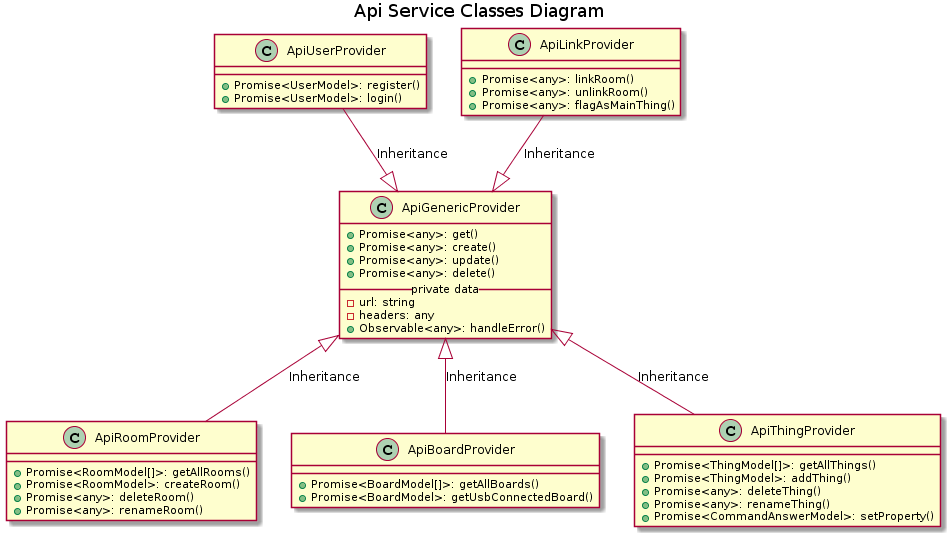
\includegraphics[height=4in]{figures/diagrams/front/architecture/api-services.png}
\caption[api-services]{API Providers Class Diagram\footnotemark}
\label{fig:api-services}
\end{figure}

\vspace{0.5cm}

De la misma forma y con el mismo objetivo que para el api provider, se crea un módulo database service (específicamente orientado para el mismo tipo de datos que la store), que permite a la store interactuar con la \gls{bbdd} local para almacenar, recuperar o borrar cualquier entrada de ese tipo. En este proyecto, de entre las posibilidades existentes, hacemos uso de la base de datos IndexedDB, propia del motor web del dispositivo. Es una base de datos No-SQL que está orientada al almacenamiento de entradas de gran tamaño, y no bloquea la entrada-salida del hilo principal, de forma que es ideal para almacenar objetos JSON, que puedan tener estructuras y tamaños variables. En particular, cada database service se creará de forma que ataque específicamente a una única tabla, nombrada con el mismo tipo de datos, con el objetivo de reforzar la mantenibilidad del código y la separación de responsabilidades. Así, de nuevo, la store se permite desconocer si sus datos deben tener una estructura, codificación o formato en particular dependiendo de las características de la \gls{bbdd}: delega esa responsabilidad en el database service, el cual debe garantizar que los datos sean devueltos a la store en el mismo formato en que fueron entregados en primera instancia. 
Los módulos database service, a diferencia de los api providers, no heredan de un mismo módulo, pero queda pendiente como una mejora posible puesto que cada uno puede ser creado con una configuración particular (como ya ocurre) y, con la excepción de algunos métodos, se puede refactorizar todos aquellos que sean comunes en una clase padre. En la Figura \ref{fig:database-service} se expone la clase que sigue RoomDatabaseService, muy similar a la que siguen el resto de database services con sus configuraciones propias. Hemos adjuntado un diagrama de cada uno de ellos en el apartado \ref{makereference4.5.4}.


\begin{figure}[hbt!]
\centering
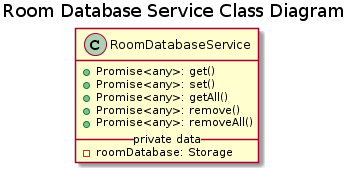
\includegraphics[height=1.5in]{figures/diagrams/front/architecture/database-service.png}
\caption[app-data]{Room Database Service Class Diagram\footnotemark}
\label{fig:database-service}
\end{figure}

\subsection{Diagramas de clases de las Stores, Models y Services}
\label{makereference4.5.4}

[EXPLICAR AQUÍ EL PROCESO DE INICIALIZACIÓN DE LA APP]

\subsection{Diagramas de clases de las Stores, Models y Services}
\label{makereference4.5.5}

\begin{figure}[hbt!]
\centering
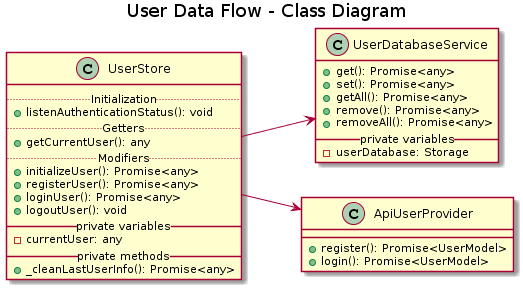
\includegraphics[height=2.5in]{figures/diagrams/front/data-flow/user.png}
\caption[user]{User Data Class Diagram\footnotemark}
\end{figure}

La user store gestiona todo lo relacionado con el login del usuario, es por ello que tiene una fuerte cooperación con el AuthService. Durante la inicialización de la aplicación, se establece una suscripción a cambios de usuarios autenticados en el AuthService con el método público \verb|listenAuthenticationStatus|.

\vspace{0.5cm}

Nuestro proyecto implementa JWT de Auth0, para la autenticación de usuario mediante tokens, lo cual agiliza el login sin necesidad de que el usuario deba introducir de nuevo sus credenciales, y puede ser parametrizado desde el backend. Durante la inicialización de la aplicación, se lanza el método \verb|initializeUser|, el cual busca en la userDB (local del dispositivo) la existencia de un JWT válido. Si lo encuentra, entonces puede pasarle el token al AuthService, el cual lo descifrará y extraerá el usuario autenticado, y establecerá el estado de autenticado del AuthService a verdadero. De esta manera, se la suscripción del \verb|listenAuthenticationStatus| da lugar a pedirle a AuthService el usuario autenticado y se establece como el usuario actual. Si no, se lanza el método privado \verb|_cleanLastUserInfo| para borrar cualquier información remanente en la aplicación móvil relativa al último usuario logado, acudiendo a todas las demás stores para que se encarguen de borrar de sus \gls{bbdd} locales la información pertinente de la que son responsables.

\vspace{0.5cm}

Además de esto, la user store posee los métodos \verb|loginUser| y \verb|registerUser| que gestionan todo lo relacionado con los intentos de registrar y de iniciar sesión contra la API remota de user mediante el userProvider. Si logra logarse correctamente, el endpoint de login devuelve un token válido que la app almacena en la userDB y que utiliza para el propósito explicado anteriormente, además de pasar al AuthService este token válido para autenticar al usuario.

\begin{figure}[hbt!]
\centering
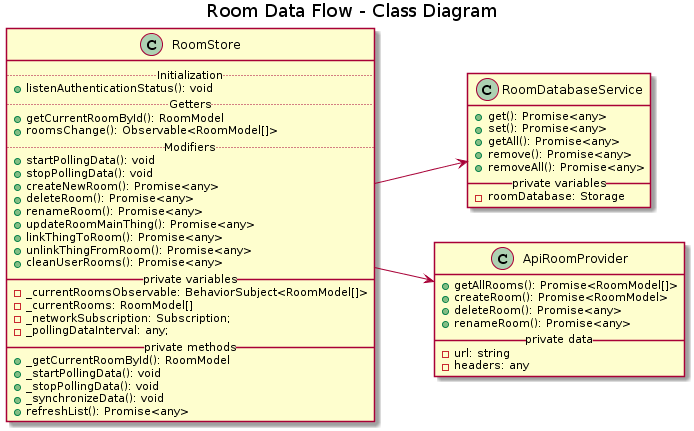
\includegraphics[height=3.5in]{figures/diagrams/front/data-flow/room.png}
\caption[room]{Room Data Class Diagram\footnotemark}
\end{figure}

\vspace{1cm}

La room store gestiona todo lo relacionado con la lista de rooms disponibles. Durante la inicialización de la aplicación, se establece una suscripción a cambios de usuarios autenticados en el AuthService con el método público \verb|listenAuthenticationStatus|; y alinea esta suscripción con otra al estado de la red con el NetworkService, de forma que, si hay conexión a la red y además el usuario está autenticado, se llama al método privado \verb|_startPollingData| (y de lo contrario, llama al \verb|_stopPollingData|).

\vspace{0.5cm}

\verb|_startPollingData| se encarga de llamar a intervalos de tiempo regulares de 5 segundos al método privado \verb|_synchronizeData|, el cual hace uso del roomProvider para obtener la lista de todas las rooms. Cada vez que interactuemos con la API remota (con cualquiera de sus métodos, y aplicable al resto de stores), ejecutaremos un flujo que consiste en recibir la información, guardarla en la roomDB y llamar al método \verb|refreshList|, que se encarga de extraer el valor actual de esa lista de la roomDB y actualizar tanto el array privado \verb|_currentRooms| como el observable \verb|_currentRoomsObservable| con el nuevo valor.

\vspace{0.5cm}

Este último paso es crucial para el flujo de datos en la aplicación y representa uno de los patrones reconocidos más útiles de los que hacemos uso en la aplicación frontend: el patrón Observer/Subscribe. La librería RXJs nos ofrece este elemento tan importante, mediante el cual cualquier flujo de la aplicación que desee hacer uso de la lista de rooms, se suscribe al observable \verb|_currentRoomsObservable| mediante el método \verb|roomsChange| de la room store. Cada vez que la room store actualice este observable, el cambio será automáticamente notificado a todos los suscriptores de dicho observable.

\vspace{0.5cm}

La room store también ofrece los métodos \verb|createNewRoom|, \verb|deleteRoom|, \verb|renameRoom|, \verb|updateRoomMainThing|, \verb|linkThingToRoom| y \verb|unlinkThingFromRoom|. Los tres primeros son autodescriptivos, interactuan con la API y siguen el mismo flujo de actualización descrito anteriormente aunque adaptado a cada caso. Los tres últimos son llamados desde la thing store como parte de unos procesos encadenados, en los cuales se requiere que se cambie información específica de alguna room en particular, pero esta vez sólo de forma local (en el dispositivo), ya que la petición al backend realizada desde la thing store ya desencadena otros flujos secundarios en el backend que actualizan la información de la room implicada. Se garantiza la alineación de datos ya que el flujo está diseñado como si de una transacción se tratara: el backend siempre tiene la información verídica, y si ocurriera algún fallo en el flujo (sea en backend o en frontend), se rechaza el flujo para evitar datos incorrectos, que en cualquier caso serán actualizados con la siguiente petición \verb|_synchronizeData|. 
La room store también expone el método \verb|cleanUserRooms|, accedido y usado desde la user store para el borrado de datos de rooms.

\begin{figure}[hbt!]
\centering
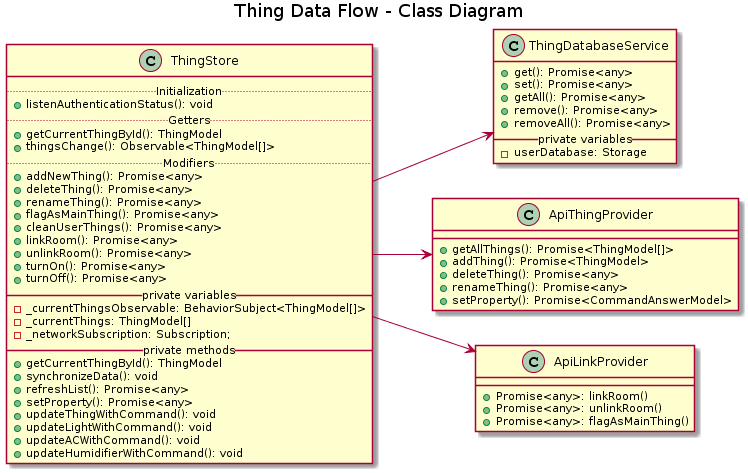
\includegraphics[height=4in]{figures/diagrams/front/data-flow/thing.png}
\caption[thing]{Thing Data Class Diagram\footnotemark}
\end{figure}

La thing store gestiona todo lo relacionado con la lista de things disponibles. Tanto la suscripción al AuthService, y al NetworkService, como el sistema de petición periódica y recuperación de datos, así como la exposición del observable a posibles suscriptores, es idéntico al de room store pero evidentemente aplicado a la lista de things, por lo cual no entraremos en detalle de nuevo.

\vspace{0.5cm}

La thing store también ofrece los métodos \verb|addNewThing|, \verb|deleteThing|, \verb|renameThing|, \verb|flagAsMainThing|, \verb|linkRoom| y \verb|unlinkRoom|, que interactuan con la API en sus métodos homónimos y siguen el mismo flujo de actualización descrito anteriormente aunque adaptado a cada caso. Los tres últimos 

La thing store también expone el método \verb|cleanUserThings|, accedido y usado desde la user store para el borrado de datos de things.


\begin{figure}[hbt!]
\centering
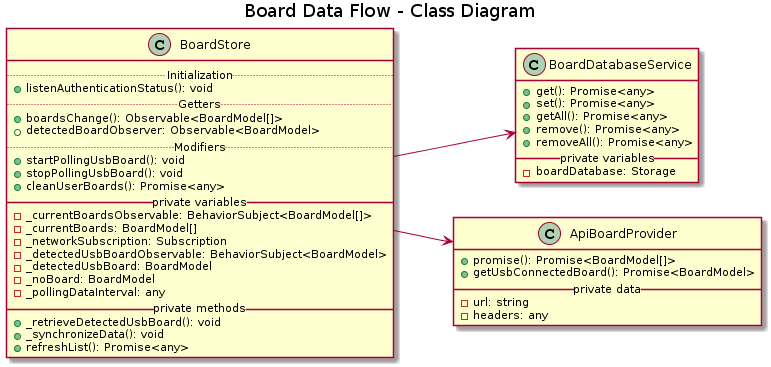
\includegraphics[height=3.5in]{figures/diagrams/front/data-flow/board.png}
\caption[thing]{Board Data Class Diagram\footnotemark}
\end{figure}

[EXPLICAR AQUÍ EL BOARD STORE]

\begin{figure}[hbt!]
\centering
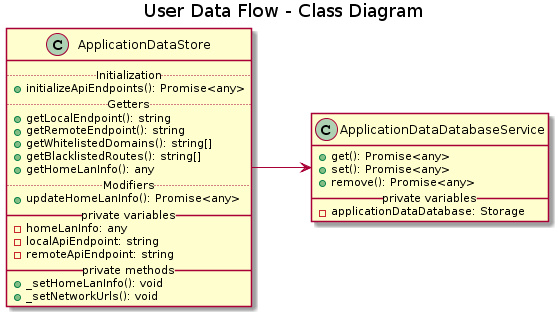
\includegraphics[height=3in]{figures/diagrams/front/data-flow/app-data.png}
\caption[app-data]{Application Data Class Diagram\footnotemark}
\end{figure}

[EXPLICAR AQUÍ EL APP DATA STORE]

\begin{figure}[hbt!]
\centering
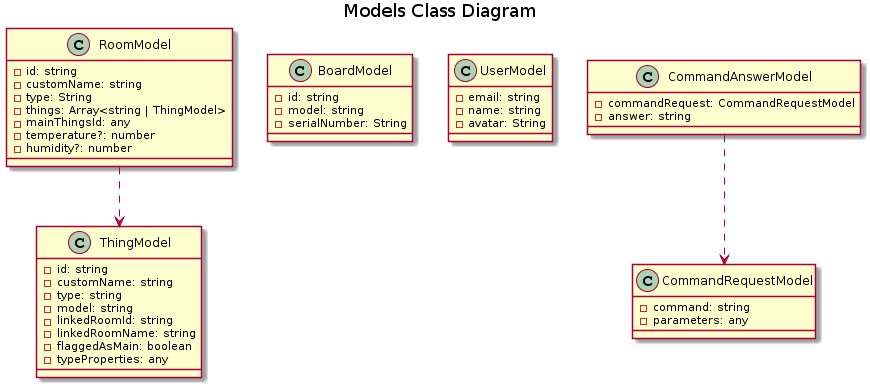
\includegraphics[height=3in]{figures/diagrams/front/architecture/models.png}
\caption[models]{Models Classes Diagram\footnotemark}
\end{figure}

[EXPLICAR AQUÍ LOS MODELS]

\begin{figure}[hbt!]
\centering
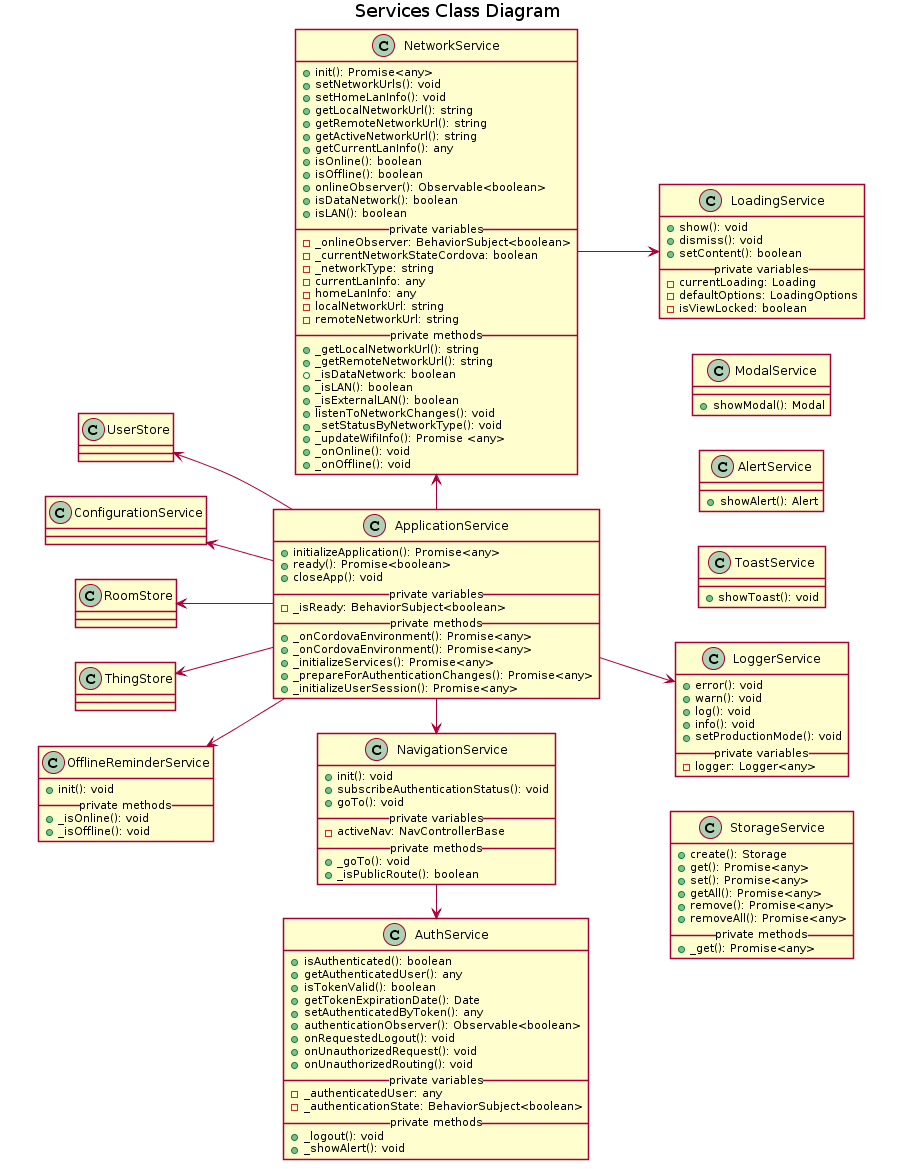
\includegraphics[height=8.5in]{figures/diagrams/front/architecture/services.png}
\caption[services]{Services Class Diagram\footnotemark}
\end{figure}

[EXPLICAR AQUÍ LOS SERVICES]

\section{Arquitectura del servidor de NodeJS}
\label{makereference4.6}

\subsection{Consideraciones previas}
\label{makereference4.6.1}

El desarrollo de la aplicación backend ha seguido la línea del stack MEAN, esto es, MongoDB, ExpressJS, Angular (éste sólo en el frontend) y NodeJS. Los beneficios de seguir dicho stack son sencillamente los de sus frameworks y herramientas: MongoDB aporta los beneficios de una \gls{bbdd} no relacional, enormemente alineado con las características del proyecto, según el cual podríamos almacenar grandes cantidades de datos con diferentes estructuras JSON bajo la misma lista de documentos sin perder velocidad de acceso o escritura; ExpressJS nos permite elaborar una API REST completa salvando los principales escollos que NodeJS podría presentarnos para tal fin, pues sus herramientas base para el tratamiento de peticiones http se presentan intrincadas y poco intuitivas; y NodeJS se beneficia de infinitas librerías de sencillo uso, constantemente probadas y actualizadas por su amplia comunidad, proveyéndonos en este caso de muchas utilidades que nos ayudan a evitar desarrollos difíciles e innecesarios no intrínsecos a una suite domótica (como es nuestro fin) y cuyos beneficios enumeraremos más adelante.

\subsection{Estructura básica}
\label{makereference4.6.2}

A grandes rasgos, la aplicación backend está estructurada en:
\begin{enumerate}
 \item Enrutadores, por lo general tendremos uno por cada nombre en nuestra API REST (los conoceremos como \textit{routers}); gracias a ExpressJS, permiten encaminar cada petición http recibida en el servidor según su tipo CRUD (GET, POST, PUT o DELETE) y la estructura de la URL asociada, para ser atendida por el método específico que debe procesar dicha petición.
 \item Controladores, por lo general tendremos uno por cada nombre en nuestra API REST (los conoceremos como \textit{controllers}); encuadran un contexto en el que se crea, manipula, sirve, guarda y destruye elementos de la estructura de datos asociada, además de exponer una serie de métodos, generalmente uno por cada posible entrada de la API para el nombre de dicha API asociado a la estructura de datos en uso.
 \item Modelos, de los que tendremos uno por cada estructura de datos existente (los conoceremos como \textit{models}); definirán la estructura JSON que debe seguir un objeto para ser incluido en una collección de MongoDB, y que utilizaremos para generar y reconocer objetos de dicho tipo de estructura de datos y poder mejorar la interacción con la \gls{bbdd} de MongoDB.
 \item Servicios, que al igual que en el proyecto frotend, ejercerán de cómodas APIs contra diferentes servicios, como pueda ser la \gls{bbdd} de MongoDB, el protocolo \gls{mqtt} y otros módulos de utilidades (los conoceremos como \textit{providers} o \textit{services}); por lo general, podrían ser prácticamente independientes y ser copiados tal cual a cualquier otro proyecto (a falta de ligeras adaptaciones que en lineas generales facilitan su explotación en cada caso) y proporcionan una capa de abstracción adicional que delimita la responsabilidad del módulo que hace uso de dicho servicio y reduce su complejidad de código.
 \item Módulos de soporte, por lo general tendremos tantos como sean necesarios, y cada uno se dedica exclusivamente a un tipo de estructura de datos (los conoceremos como helpers); ofrecen sus métodos tanto a su controller asociado como a otros controllers, de forma desacoplada con el fin de aligerar la carga de código del controller asociado.
 \item Módulos intermediarios, que aportan utilidades adicionales a la hora de procesar peticiones http (los conoceremos como \textit{middlewares}); gracias a ExpressJS, permitirán enriquecer el tratamiento de dichas peticiones para establecer filtros adicionales o transformaciones de los datos de la petición.
 \item Archivos de configuración y de constantes, que permitirán aislar adecuadamente el uso de constantes útiles a lo largo de toda la aplicación, de una forma centralizada, independiente y de fácil acceso y modificación.
\end{enumerate}

Con el fin de comprender el esquema utilizado y establecer una alineación con el frontend, la nomenclatura utilizada para cada tipo de datos será la misma que en el proyecto cliente.

\subsection{Flujo de enrutado de las peticiones HTTP}
\label{makereference4.6.3}

\begin{figure}[hbt!]
\centering
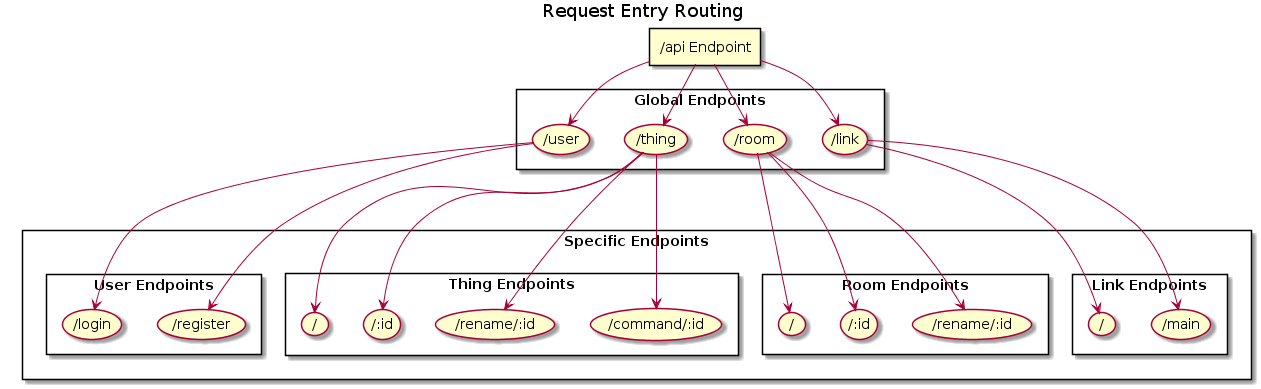
\includegraphics[height=2.5in]{figures/diagrams/back/router-flow/api-entry.png}
\caption[api-entry]{Base API Entry Schema\footnotemark}
\label{fig:back-api-entry}
\end{figure}

Como hemos explicado anteriormente, ExpressJS es utilizado para el enrutado de toda petición HTTP que alcance la aplicación backend. Durante la inicialización del servidor, mediante el método \verb|listen| en el \verb|server.js| se utiliza el objeto \verb|app| expuesto en el \verb|src/app.js| (un objeto generado por el framework ExpressJS) para generar un servidor que atenderá todas las peticiones HTTP en el puerto que se le configure, en este caso, se ha designado el puerto 3000.
\vspace{0.5cm}
Posteriormente, se lanza el setup del enrutador con el método \verb|setupRouting| del módulo \verb|router.js|, el cual se encarga de importar todos los routers existentes y vincularlos a cada uno de los endpoints que serán atendidos mediante el método \verb|use| del objeto \verb|app|. Así, suponiendo que se recibe una petición http con la ruta \verb|/api/thing|, ésta será redirigida al router \verb|thingRouter| mediante el método y sus parámetros \verb|use(ROUTER_CONFIG.EP_GLOBAL.THINGS, thingRouter)|. El primer nivel de encaminamiento de las peticiones es tal que el mostrado en la Figura \ref{fig:back-api-entry}.
\vspace{0.5cm}
Una vez la petición ha sido encaminada a un router en particular, entramos en el segundo nivel de encaminamiento. En este punto, el router se encarga de importar el controller específico para su tipo de datos y de encaminar cada endpoint a la función final de un controller que atenderá a dicha petición. ExpressJS nos permite registrar dicha función a ejecutar para unas características particulares de petición, de forma que con unos sencillos métodos, podremos asociar dicho método dependiendo del tipo CRUD de la petición atendida y de las características de su URL. Así, suponiendo que nuestro \verb|thing.router.js| atiende una petición PUT en la url \verb|/api/thing/rename/:id|, mediante el método \verb|put| podremos encaminar dicha petición a ser atendida por el método \verb|renameThing| del \verb|thing.controller.js|. Este segundo nivel de encaminamiento de las peticiones es tal que el mostrado en cada una de las figuras siguientes, brevemente descrito para cada endpoint.

\begin{figure}[hbt!]
\centering
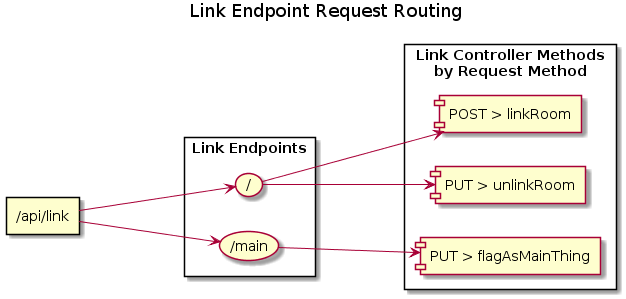
\includegraphics[height=2.5in]{figures/diagrams/back/router-flow/link-endpoints.png}
\caption[link-endpoints]{Link API Schema\footnotemark}
\end{figure}

Para el endpoint \verb|/api/link|, se asocian 3 entradas atendidas por el \verb|link.router.js|:
\begin{enumerate}
\item En la ruta \verb|/api/link/|, las peticiones POST serán atendidas por el método \verb|linkRoom|.
\item En la ruta \verb|/api/link/|, las peticiones PUT serán atendidas por el método \verb|unlinkRoom|.
\item En la ruta \verb|/api/link/main|, las peticiones PUT serán atendidas por el método \verb|flagAsMainThing|.
\end{enumerate}

\begin{figure}[hbt!]
\centering
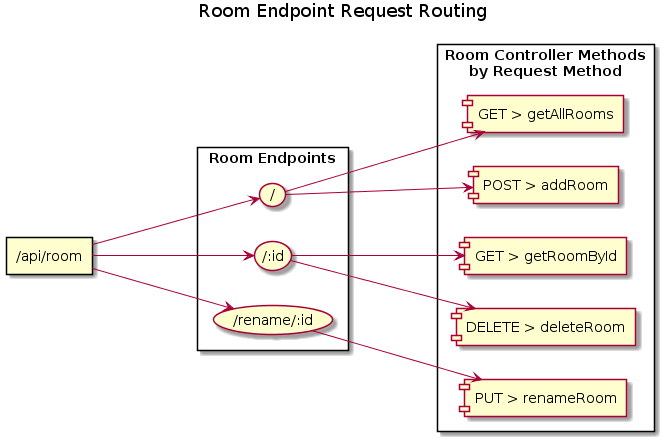
\includegraphics[height=2.5in]{figures/diagrams/back/router-flow/room-endpoints.png}
\caption[room-endpoints]{Room API Schema\footnotemark}
\end{figure}

Para el endpoint \verb|/api/room|, se asocian 5 entradas atendidas por el \verb|room.router.js|:
\begin{enumerate}
\item En la ruta \verb|/api/room/|, las peticiones GET serán atendidas por el método \verb|getAllRooms|.
\item En la ruta \verb|/api/room/|, las peticiones POST serán atendidas por el método \verb|addRoom|.
\item En la ruta \verb|/api/room/:id|, las peticiones GET serán atendidas por el método \verb|getRoomById|.
\item En la ruta \verb|/api/room/:id|, las peticiones DELETE serán atendidas por el método \verb|deleteRoom|.
\item En la ruta \verb|/api/room/rename/:id|, las peticiones PUT serán atendidas por el método \verb|renameRoom|.
\end{enumerate}

\begin{figure}[hbt!]
\centering
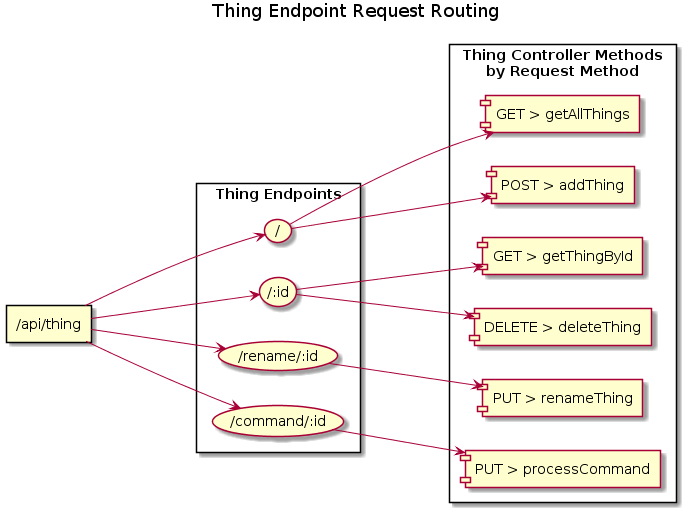
\includegraphics[height=2.5in]{figures/diagrams/back/router-flow/thing-endpoints.png}
\caption[thing-endpoints]{Thing API Schema\footnotemark}
\end{figure}

Para el endpoint \verb|/api/thing|, se asocian 6 entradas atendidas por el \verb|thing.router.js|:
\begin{enumerate}
\item En la ruta \verb|/api/thing/|, las peticiones GET serán atendidas por el método \verb|getAllThings|.
\item En la ruta \verb|/api/thing/|, las peticiones POST serán atendidas por el método \verb|addThing|.
\item En la ruta \verb|/api/thing/:id|, las peticiones GET serán atendidas por el método \verb|getThingById|.
\item En la ruta \verb|/api/thing/:id|, las peticiones DELETE serán atendidas por el método \verb|deleteThing|.
\item En la ruta \verb|/api/thing/rename/:id|, las peticiones PUT serán atendidas por el método \verb|renameThing|.
\item En la ruta \verb|/api/thing/command/:id|, las peticiones PUT serán atendidas por el método \verb|processCommand|.
\end{enumerate}

\begin{figure}[hbt!]
\centering
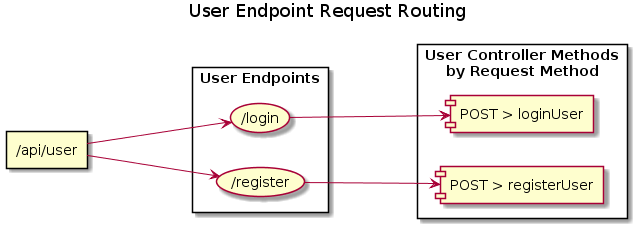
\includegraphics[height=2.5in]{figures/diagrams/back/router-flow/user-endpoints.png}
\caption[user-endpoints]{User API Schema\footnotemark}
\end{figure}

Para el endpoint \verb|/api/user|, se asocian 2 entradas atendidas por el \verb|user.router.js|:
\begin{enumerate}
\item En la ruta \verb|/api/link/login|, las peticiones POST serán atendidas por el método \verb|loginUser|.
\item En la ruta \verb|/api/link/register|, las peticiones POST serán atendidas por el método \verb|registerUser|.
\end{enumerate}

\begin{figure}[hbt!]
\centering
\includegraphics[height=2.5in]{figures/diagrams/back/router-flow/board-endpoints.png}
\caption[board-endpoints]{Board API Schema\footnotemark}
\end{figure}

Para el endpoint \verb|/api/board|, se asocian 2 entradas atendidas por el \verb|board.router.js|:
\begin{enumerate}
\item En la ruta \verb|/api/board/|, las peticiones GET serán atendidas por el método \verb|getAllBoards|.
\item En la ruta \verb|/api/board/detect|, las peticiones GET serán atendidas por el método \verb|getUSBConnectedBoard|.
\end{enumerate}

[HABLAR AQUÍ DE MIDDLEWARES]
[passport.middleware.js]


Toda petición http que no sea encaminada a un método mediante esta metodología será automáticamente rechazada. Esto permite controlar severamente los caminos por los cuales se ejecutará una lógica en base a una petición http, y por ende constituye una medida de seguridad adicional por el principio básico de conocer y controlar todas las posibles entradas al servidor con un flujo único y específico para cada una de ellas, para minimizar brechas de seguridad.

\subsection{Diagramas de clases de los Controllers, Helpers, Models y Providers}
\label{makereference4.6.4}

[HABLAR AQUÍ DE CONTROLLERS]

[core.controller.js
  prepareCoreInstances,
  setupCoreMonitors,
  _launchStoredSubscriptions,
  _releaseDaemons
]

[room.controller.js
initializeRooms
roomDaemon
getAllRooms
getRoomById
addRoom
deleteRoom
renameRoom
]

[thing.controller.js
  initializeThings,
  getThingsByRoom,
  thingDaemon,
  addThing,
  getAllThings,
  getThingById,
  deleteThing,
  renameThing,
  processCommand
]

[link.controller.js
  linkRoom,
  unlinkRoom,
  flagAsMainThing
]

[board.controller.js
  getAllBoards,
  getUSBConnectedBoard
]

[user.controller.js
  getAllBoards,
  getUSBConnectedBoard
]

[HABLAR AQUÍ DE HELPERS]
[thing.helper.js
  translateCommand,
  getThingControllerInstance,
  generateSubscriptionData,
  getModelStructure,
  getDHT11AvgInfo,
  getMQ135AvgInfo
]

[HABLAR AQUÍ DE MODELS]

[Modelo Board, diagrama y corresponde a la collección Boards]
[Modelo Room, diagrama y corresponde a la collección Rooms]
[Modelo Thing, diagrama y corresponde a la collección Things]
[Modelo User, diagrama y corresponde a la collección Users]


[HABLAR AQUÍ DE PROVIDERS]

[mongo.db.js _connect]

[mqtt.service.js
  initializeClient,
  stopClient,
  addSubscription,
  removeSubscription,
  publish
  
  _loadSubscriptions
  _subscribeTopic
  _unsubscribeTopic
  _publishTopic
  _initMessageListener
  _formTopic
  _findSubscriptionIndex
  _processMessage
  ]
  
  [shell.service.js 
  compileAndUploadToBoard
  _execAsync
  ]

  [usb.service.js 
  initListening,
  stopListening,
  getCurrentConnectedUSB,
  ]

\section{Instalación y configuración del nodo principal}
\label{makereference4.7}
 Utilizando los repositorios de distribuciones oficiales de Sistemas operativos de Raspberry Pi, descargamos la versión ``Lite'' de Raspbian. Para establecer una conexión SSH por terminal es necesario crear un fichero con nombre \verb|ssh| en la raiz de la unidad de almacenamiento donde previamente se haya montado la imagen descargada. La distribución de Raspbian originalmente estaba configurada por defecto con la conexión de SSH abierta en el puerto 22, pudiendo accederse con el usuario \verb|pi| y la contraseña \verb|raspberry|. Este dato era ignorado por los usuarios menos experimentados y esto supuso una brecha de seguridad en todos las distribuciones que no fueron configuradas a posteriori por los usuarios según las indicaciones de la propia \href{https://www.raspberrypi.org/documentation/configuration/security.md}{documentación de Raspberry}~\cite{securingyourraspberrypi}. En el primer arranque del SO de la Raspberry se establecerán las configuraciones básicas para las sucesivas conexiones SSH basadas en autenticación con claves privadas.

 De las estrategias disponibles para esta configuración, se crearán las claves en el equipo remoto que se conectará a la Raspberry, entregando mediante la primera conexión SSH con terminal la clave pública y almacenando la clave privada en el equipo remoto, reduciendo así el riesgo de ser expuesta fuera del dominio local del equipo. Para disponer de flexibilidad de conexión independientemente del SO del equipo remoto, la clave privada tendra un formato OpenSSH, fácil de incluir en SO Windows ya sea mediante conversión de la clave a formato PPK o como fichero accesible para aplicaciones de desarrollo, transferencias de ficheros, y/o control de versiones que integran conexiones SSH configurables (GitHub, Filezilla, Eclipse, etc). Los pasos necesarios para establecer conexiones cifradas robustas pueden encontrarse en el Anexo A seccion de implementación del Gateway.

Establecemos la capacidad de la Raspberry Pi 3 para su módulo de comunicación wifi de actuar como punto de acceso en modo NAT~\cite{raspberrypiasaccesspoint}. Se configura una red con acceso vía usuario y contraseña, con WPA2 y gestión de claves WPA-PSK. De esta forma, el nodo será capaz de desplegar una red inalámbrica que permitirá a otros dispositivos incorporarse a la suite domótica.

En orden de subir sketcs a una Arduino desde una Raspeberry Pi, es necesario instalar las paqueterías del compilador sudo apt-get install arduino-mk, tras la instalación, en la ruta /usr/sahre/arduino pueden encontrar binarios y una capeta llamada examples que permiten cargan sketchs inmediatamente para comprobar el correcto funcionamiento del la placa microcontroladora. Para compilar dicho sketcs se necesita hacer referencia al fichero arduino.mk. De los ejemplo podemos verificar rampidamente el correcto funcionamiento de la microcontroladores utilizamos el mas básico de los \gls{sketch}, situado en /usr/share/arduino/examples/01.Basic/Blink/Blink.ino, este ejemplo es muy básico, un loop que enciende y apaga el led integrado en la placa microcontroladora cada 1000 milisegundos. Este , es por defecto el sketch que generelamente los disitntos fabricantes de placas microcontroladoras de con procesador ATmega328P suelen dejar cargado a modo de test. Alterando el valor basico de sleep entre lineas de encendido y apagado a un valor menor como 50 milisegundos se puede comprobar si la comunicación del puerto com, y el compilador suben correctamente el codigo a la placa. Es importante verificar este punto antes de continuar y esta simple prueba cofirma que la configuración actual esta bien.

Para facilitar el proceso de subida de codigo a la placa de arduino, crearemos un Makefile hijo que enlace parametros al compilador.


Ahora bien, tengamos en cuenta que las especificaciones del modulo esp8266 de wifi conectado a Arduino requieren de una alimentación de 3.3V que pueden ser suministrados por la placa microcontroladora, sin embargo, esto nos deja con un problema de intensidad en la alimentación del modulo, ya que el pin de 3.3V disponible en la placa posees un amperaje de 50mA y se requieren de unos 200mA para garantizar una comunicación estable.


mqtt
\url{https://theembeddedlab.com/tutorials/install-mosquitto-on-a-raspberry-pi}
\verb|-h BROKER -t TOPIC|

\verb|mosquittosub -h localhost -t casa/comedor/temperatura|
\verb|mosquittopub -h localhost -t casa/comedor/temperatura -m "Temperatura: 25ºC"|


usando comunicacion cifrada en nodeucm esp8266
https://github.com/esp8266/arduino-esp8266fs-plugin
cifrado tls open source
\url{https://github.com/esp8266/Arduino/blob/master/libraries/ESP8266WiFi/src/WiFiClientSecure.h#L52-L66}
\cleardoublepage

\chapter{Implementación}
\label{makereference5}



\section{Instalación y configuración del nodo principal}
\label{makereference5.1}
 Utilizando los repositorios de distribuciones oficiales de Sistemas operativos de Raspberry Pi, descargamos la versión ``Lite'' de Raspbian. Para establecer una conexión SSH por terminal es necesario crear un fichero con nombre \verb|ssh| en la raiz de la unidad de almacenamiento donde previamente se haya montado la imagen descargada. La distribución de Raspbian originalmente estaba configurada por defecto con la conexión de SSH abierta en el puerto 22, pudiendo accederse con el usuario \verb|pi| y la contraseña \verb|raspberry|. Este dato era ignorado por los usuarios menos experimentados y esto supuso una brecha de seguridad en todos las distribuciones que no fueron configuradas a posteriori por los usuarios según las indicaciones de la propia \href{https://www.raspberrypi.org/documentation/configuration/security.md}{documentación de Raspberry}~\cite{securingyourraspberrypi}. En el primer arranque del SO de la Raspberry se establecerán las configuraciones básicas para las sucesivas conexiones SSH basadas en autenticación con claves privadas.

 fiware citas bitpex

 De las estrategias disponibles para esta configuración, se crearán las claves en el equipo remoto que se conectará a la Raspberry, entregando mediante la primera conexión SSH con terminal la clave pública y almacenando la clave privada en el equipo remoto, reduciendo así el riesgo de ser expuesta fuera del dominio local del equipo. Para disponer de flexibilidad de conexión independientemente del SO del equipo remoto, la clave privada tendra un formato OpenSSH, fácil de incluir en SO Windows ya sea mediante conversión de la clave a formato PPK o como fichero accesible para aplicaciones de desarrollo, transferencias de ficheros, y/o control de versiones que integran conexiones SSH configurables (GitHub, Filezilla, Eclipse, etc). Los pasos necesarios para establecer conexiones cifradas robustas pueden encontrarse en el Anexo A seccion de implementación del Gateway.

Establecemos la capacidad de la Raspberry Pi 3 para su módulo de comunicación wifi de actuar como punto de acceso en modo NAT~\cite{raspberrypiasaccesspoint}. Se configura una red con acceso vía usuario y contraseña, con WPA2 y gestión de claves WPA-PSK. De esta forma, el nodo será capaz de desplegar una red inalámbrica que permitirá a otros dispositivos incorporarse a la suite domótica.

Descargamos la paquetería de Adafruit para el primer sensor de pruebas, el sensor DTH11 de temperatura y humedad.
Se requiere un montaje sencillo.
\begin{figure}[hbt!]
\centering
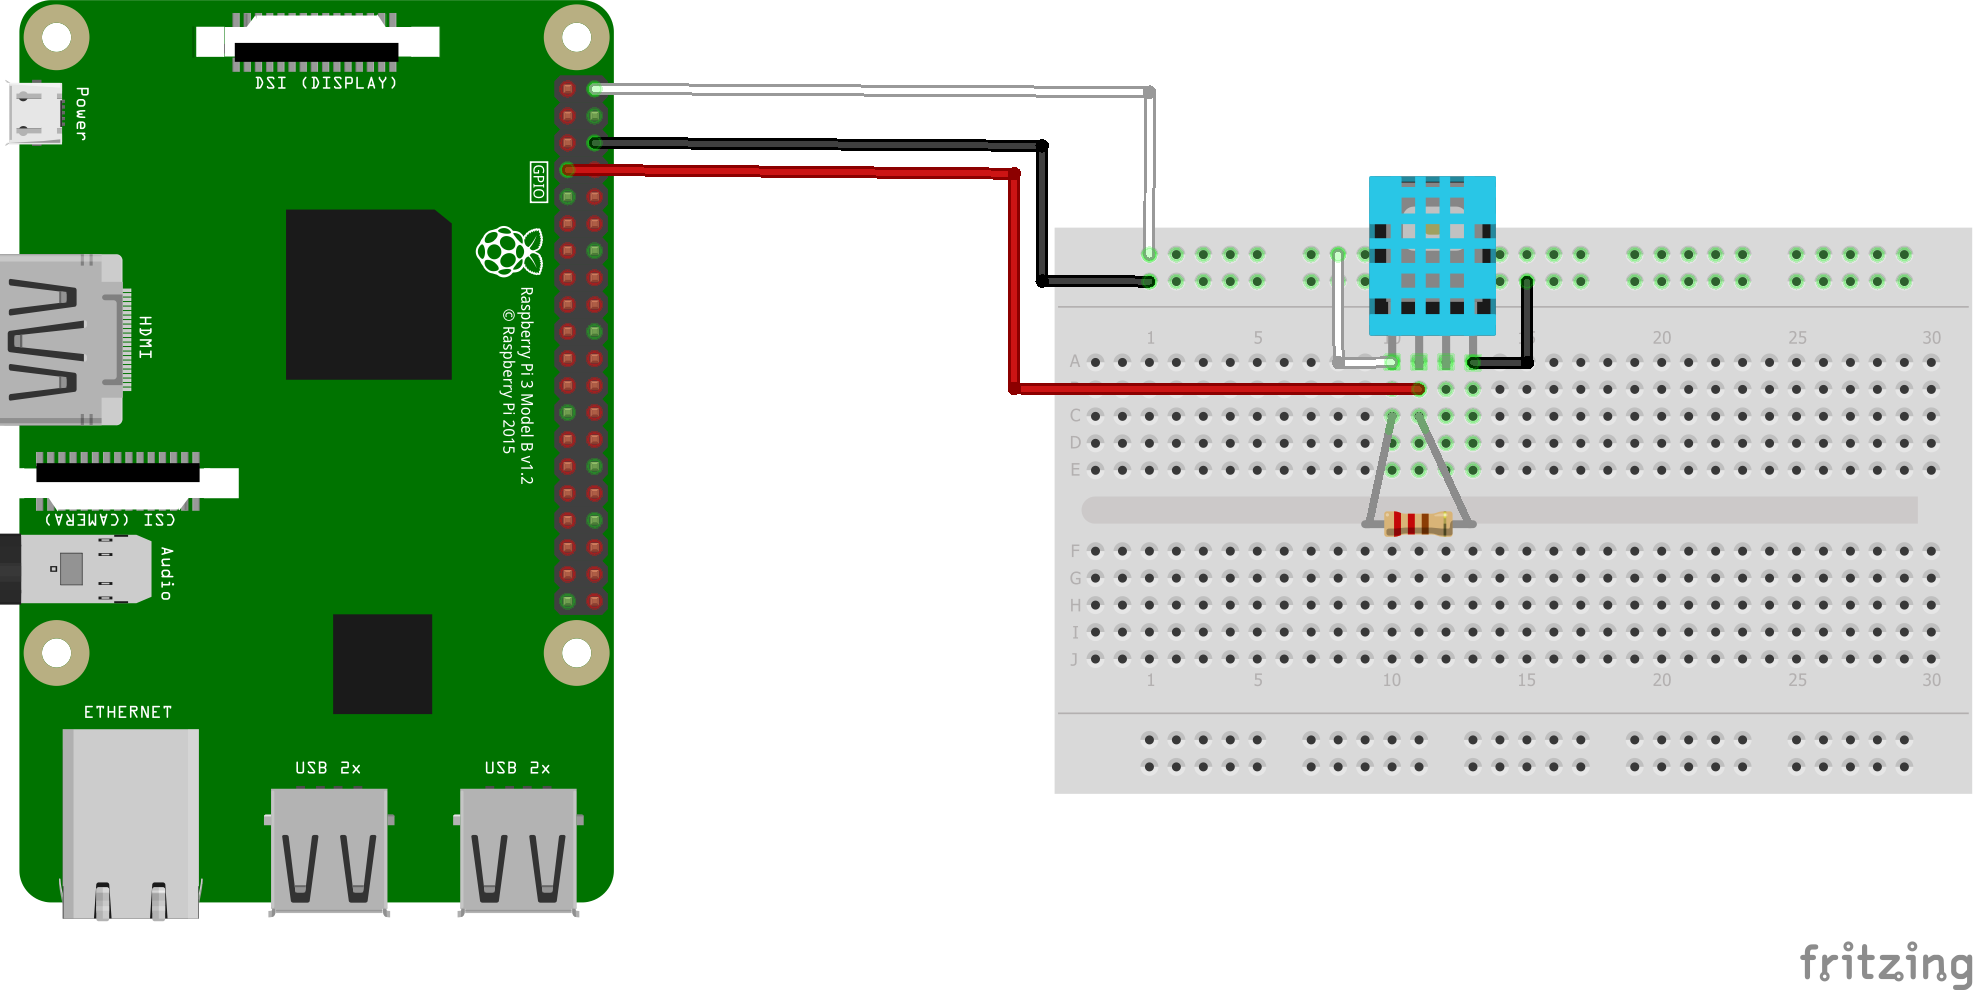
\includegraphics[height=2.5in]{figures/nodo_1.png}
\end{figure}

Clonamos la librería del sensor, nos ubicamos en la ruta descargada \verb|cd Adafruit_Python_DHT| e instalamos la librería \verb|sudo python setup.py install|, previamente instalamos las dependencias de la librería para su instalación \verb|sudo apt-get install python-setuptools| considerando que tenemos la versión de python 2.7.3, esto permitirá instalar la librería de python para el sensor DHT version 1.4. Se debe realizar una prueba de contacto con un script que nos muestre la información por pantalla para verificar que las conexiones del sensor a la rapsberry son correctos. Este primer script es un bucle infinito de mediciones de temperatura y humedad cada poco segundos. Hay una justificación para elegir un bucle sobre una única medida del sensor y está fundamentada en el margen de error inicial de las medidas. Si bien el sensor DTH11 es una opción muy común por su bajo coste y facilidad de implementación (este sensor se caracteriza por tener la señal digital calibrada por lo que asegura una alta calidad y una fiabilidad a lo largo del tiempo, ya que contiene un microcontrolador de 8 bits integrado. Está constituido por dos sensores resistivos (NTC y humedad) - revisar esta info y contrastarla contra ésta: \url{ https://programarfacil.com/blog/arduino-blog/sensor-dht11-temperatura-humedad-arduino/}), ademas de manejar señales digitales que no se ven afectadas por las fluctuaciones de voltaje, tiene algunas contrapartidas que deben tenerse en cuenta. Se necesita un tiempo mínimo de espera entre medidas (de al menos 1 segundo), hecho que no agrava particularmente su desempeño en entornos cerrados como una casa, ya que las variaciones de temperatura y humedad no son bruscas, aun así existen estrategias para reducir estos tiempos, por ejemplo, usar la función millis() de Arduino, el cual nos da el tiempo en milisegundos desde que empieza a ejecutarse el código, De esta forma evitamos la pausa de los 2 segundos, pero no el tiempo que demora en hacer la lectura, que es de aproximadamente  250 milisegundos, el cual lo pueden notar si realizan el ejemplo anterior, en donde se hace parpadear el led interno de la placa (Pin 13) con pausas de 100ms (tomado de \url{https://naylampmechatronics.com/blog/40_Tutorial-sensor-de-temperatura-y-humedad-DHT1.html}). Otro problema que abordar es que las primeras lecturas tienen un margen de error de unos +-2 grados Celsius y +-5\% de humedad relativa en las primeras 4 lecturas. Esto generará un problema a la hora de tomar lecturas instantáneas si el sensor no se encuentra ya operando cuando se solicita el dato. Como estrategia, haremos que el sensor tome medidas indefinidamente y los vuelque en un fichero/BBDD para recortar los tiempo de respuesta, evitando así esperar a que el sensor haga la toma de medidas en el momento+ de solicitud y sacándolas en su lugar del último registro que tengamos. Un último problema con el que hay que lidiar es su baja precisión limitada a enteros, por lo que no podemos esperar obtener un dato preciso a la décima de la temperatura y humedad. Esto sin embargo no es un problema real dada la naturaleza del proyecto, ya que no necesitamos un grado de precisión menor a la unidad para tomar acciones o informar al usuario.

En orden de subir sketcs a una arduino desde una Raspeberry Pi, es necesario isntalar las paqueterias del compilardor \verb|sudo apt-get install arduino-mk|, tras la instalación, en la ruta \verb|/usr/sahre/arduino| pueden encontrar binarios y una capeta llamada \verb|examples| que permiten cargan sketchs inmediatamente para comprobar el correcto funcionamiento del la placa microcontroladora. Para compilar dicho sketcs se necesita referenciar el fichero arduino.mk. De los ejemplo podemos verificar rampidamente el correcto funcionamiento de la microcontroladores utilizamos el mas basico de los sketcs, situado en \verb|/usr/share/arduino/examples/01.Basic/Blink/Blink.ino|, este ejemplo es muy basico, un loop que enciende y apaga el led integrado en la placa microcontroladora cada 1000 milisegundos. Este , es por defecto el sketch que generelamente los disitntos fabricantes de placas microcontroladoras de con procesador ATmega328P suelen dejar cargado a modo de test. Alterando el valor basico de sleep entre lineas de encendido y apagado a un valor menor como 50 milisegundos se puede comprobar si la comunicación del puerto com, y el compilador suben correctamente el codigo a la placa. Es importante verificar este punto antes de continuar y esta simple prueba cofirma que la configuración actual esta bien.

Para facilitar el proceso de subida de codigo a la placa de arduino, crearemos un Makefile hijo que enlace parametros al compilador.


Ahoera bien, tengamos en cuenta que las especificaciones del modulo esp8266 de wifi conectado a arduino requieren de una laimentación de 3.3V que pueden ser suministrados por la placa microcontroladora, sin embargo, esto nos deja con un problema de intensidad en la alimentación del modulo, ya que el pin de 3.3V disponible en la placa posees un amperaje de 50mA y se requieren de unos 200mA para garatizar una comunicación estable.

\cleardoublepage

\chapter{Casos de Estudio}
\label{makereference6}

\cleardoublepage

\chapter{Conclusión}
\label{makereference7}

Hemos creado un prototipo escalable que permite integrar soluciones de manera escalonada. Para nuestra bodega, originalmente el objetivo solo trataba de observar las temperatura y humedad de la estancia, en siguientes iteraciones, se plantea automatizar ciertos aspectos del control como la temperatura manipulando electrodomésticos que permitan controlar ambos factores. EL sistema de iluminación dispone ahora ademas de un control de luz mas automatizado, lo cual aporta confort, gracias al control remoto de la \gls{app}.

El estudio requerido para la creación de una suite domótica ha representado un reto dada la extensión de opciones tecnológicas, estándares establecidos y protocolo de arquitectura y comunicación disponibles. Aun no habiendo podido experimentar con pruebas reales todos los estudios planteados en el estado del arte, podemos confirmar una selección adecuada de tecnologías para abordar un proyecto de \gls{iot} que enfrente los problemas característicos de una suite domótica.

zigbee
nodeucm
node y mongo


% +-------------------------------------------------------------------------+
% | References                                                              |
% +-------------------------------------------------------------------------+

% +-------------------------------------------------------------------------+
% | In order for WinEDT to index references correctly, it has to know where |
% | the file resides.  The following command is prefaced by %, and will be  |
% | ignored completely by LaTeX.  However, WinEDT will use this line to     |
% | access the external .bib bibliography file.  Also note that WinEDT can  |
% | read file path names with either "\" or "/" - LaTeX, however, doesn't   |
% | like "\", so it's easier to store a path name in the "Unix" style.      |
% +-------------------------------------------------------------------------+

%Included for Gather Purpose only.  Do NOT uncomment:
%input "references.bib"

% +--------------------------------------------------------------------+
% | This template uses the BibTeX program to format references.  The
% | 3 lines below create a separate Bibliography section and add
% | an entry for "Bibliography" to the Table of Contents.  The actual
% | data for your references (author, title, journal, date, etc.) are
% | entered in the references.bib file.  See that file for information
% | on how to enter references.
% +--------------------------------------------------------------------+

\printglossary

\bibdata{references}
\bibliography{references}
\addcontentsline{toc}{chapter}{Bibliography}

% +--------------------------------------------------------------------+
% | Finally, we generate the appendix.  To add or delete appendices,
% | add or remove the line
% |
% |     \input{appendixX.tex}
% |
% | where "X" is the letter designation of the Appendix (A, B, C, etc.)
% | You should have one \input{appendixX.tex} line and a corresponding
% | file appendixX.tex for each appendix.                                 |
% +--------------------------------------------------------------------+


\appendix
% +--------------------------------------------------------------------+
% | Appendix A Page (Optional)                                         |
% +--------------------------------------------------------------------+


\cleardoublepage

% +--------------------------------------------------------------------+
% | Enter text for your Appendix page in the space below this box.     |
% |                                                                    |
% +--------------------------------------------------------------------+

\chapter{Intrucciones de configuración}
\label{AppendiA:Key1}

\section{Proceso de configuración de conexion SSH para el Gateway}
\label{AppendiA:Key2}

En Windows puede utilizarse aplicaciones de gestión de claves como 'puttygen'. En la sección de parámetros de generación de las claves se define SSH-2 RSA de 2048bits y en la sección de acciones pulsamos en 'genérate'. Tras unos movimientos aleatorios de ratón se generará la clave pública en el área de texto. Se deben guardar ambas claves mediante los botones 'save public key' y 'save private key'. Esta última será guardada con una contraseña definida en los inputs de la aplicación para tal fin. La clave privada será almacenada en formato PPK para ser rápidamente usada por aplicaciones de conexión por terminal remota como 'PUTTY'. Es recomendable exportar dicho fichero a formato OpenSSH mediante la misma aplicación de generación de claves, en la sección 'Conversions' del menú desplegable y seleccionando la opción 'Export OpenSSH key', definimos un nombre para el fichero de salida y pulsamos 'save'. Esta misma operación puede realizarse desde una terminal de un SO Linux mediante el comando \verb|ssh-keygen -t rsa| que generará por defecto la claves en el directorio \path{/home/username/.ssh/} bajo el nombre \verb|id_rsa.pub| e \verb|id_rsa| para las claves pública y privada respectivamente.

\vspace{1cm}

Al no disponer de interfaz mediante dispositivos I/O para una acceso local con la Raspberry, es necesario establecer una primera conexión de terminal remoto mediante SSH con usuario y contraseña. Este primer acceso nos permite establecer las reglas de conexión que se usarán en adelante en el fichero de configuración en la ruta \path{/etc/ssh/sshd_config} asi como la configuracion de cuentas de usuarios.

\vspace{1cm}

Las distribuciones de Raspbian disponen del usuario por defecto \verb|pi|. Esta cuenta de usuario esta incluido dentro del grupo de usuarios \verb|sudo|. En adelante se operará con una cuenta distinta que ha de generarse manualmente y adicionalmente eliminar la cuenta del usuario \verb|pi| para limitar brechas de seguridad. Como primer paso, crear el usuario \verb|sudo adduser edomus| e incluir al usuario en el grupo de usuarios \verb|sudo|. El fichero por defecto creado durante la instalación de la distribución situado en \path{/etc/sudoers} dispone de la directiva \verb|includedir /etc/sudoers.d| que debe ser descomentada en el fichero de configuración de \verb|sudo sudoers|, mediante el comando \verb|visudo|. Es necesario crear un fichero en la ruta \path{/etc/sudoers.d} con el siguiente formato de nombre \verb|010_edomus-nopasswd| cuyo contenido incluya la siguiente linea \verb|edomus ALL=(ALL) NOPASSWD: ALL| una vez se haya habilitado la directiva. Tras realizar las comprobaciones de que el nuevo usuario puede operar sin problemas con la nueva configuración de permisos, se elimina el fichero de permisos existente en \path{/etc/sudoers} para el usuario \verb|pi|, y su eliminación del sistema con el comando \verb|sudo deluser -remove-home pi|.

\vspace{1cm}

Para realizar la comunicación remota por terminal en SSH de manera más segura y cómoda, incluiremos un fichero con el contenido de la clave pública en una ruta manualmente definida dentro del 'home' del usuario edomus.

\vspace{1cm}

En concreto modificaremos el puerto de entrada para redirigir la conexión del puerto por defecto 22 a un valor más elevado (como por ejemplo el 45021). Esta decisión tiene como objetivo retrasar las técnicas de sondeo de puertos de un atacante hacia un servidor que admite conexiones externas. Un bot programado para encontrar servidores y marcarlos como objetivo de ataques escaneara puertos mediante evaluación de respuestas con paquetería ICMP. Igualmente un atacante puede determinar la naturaleza de los servicios ofrecidos por un servidor mediante herramientas como \verb|Nmap|, al establecer valores elevados en los puertos, un rastreo incremental desde los valores más bajos llevará mas tiempo, permitiendo a las soluciones de seguridad (como un firewalls) del servidor detectar el ataque con margen mayor de tiempo.

\vspace{1cm}

En este mismo fichero establecemos unos límites concretos en los valores de tiempo de gracia \verb|LoginGraceTime 5| de apenas 5 segundos, impedimos el acceso del usuario root desde una conexión externa \verb|PermitRootLogin no|, limitamos el número de intentos de conexión \verb|MaxAuthTries 3| y el número máximo de sesiones simultáneas \verb|MaxSessions|. Para admitir las conexiones SSH mediante una autentificación con clave es necesario habilitar la autentificación de clave pública \verb|PubkeyAuthentication yes| y definir la ruta del fichero con la clave publica almacenada localmente en el servidor \verb|AuthorizedKeysFile| \path{.net/.aut} (véase que en este caso hemos definido una ruta manualmente indicando que la clave pública se encuentra en un fichero oculto nombrado \verb|aut| en la ruta \path{/home/pi/.net}). Como refuerzo adicional configuramos el servidor para denegar todo intento de conexión mediante contraseña plana \verb|PasswordAuthentication no|, y adicionalmente limitar el acceso sólo a las cuentas de usuarios designadas \verb|AllowUsers edomus|. Definidos los nuevos cambios de configuración, es necesario reiniciar el servicio.


\label{AppendiA:Key3}
\section{Instalación de mosquito}
Lo primero es descargar la signing key o clave de firma utilizando el comando wget.Añadimos la clave para a una lista para autenticar el paquete que vamos a descargar más tarde.

\begin{verbatim}
sudo wget http://repo.mosquitto.org/debian/mosquitto-repo.gpg.key
sudo apt-key add mosquitto-repo.gpg.key
sudo apt-get update 
sudo apt-get install mosquitto
\end{verbatim}

Si durante el proceso de instalación se encontrases errores de dependencias, algo común en distribuciones Raspbian, puede revisarse el apartado de Trobuleshooting.


\section{Proceso de instalación y configuración de Arduino en linea de comandos}
\label{AppendiA:Key4}

Al tratarse el \gls{so} del nodo principal de un entorno de terminal \gls{cli}, no podemos utilizar el \gls{ide} de Arduino de escritorio, que pese a disponer de compilaciones para la mayoría de distribuciones de \verb|GNU\Linux|, se requiere de un entorno gráfico para  para su ejecución. Sin embargo, en 2018 la compañía de Arduino anuncio arduino-cli, que se presenta como la alternativa \gls{cli} del \gls{ide} de Arduino. Aunque sigue siendo una herramienta de software aun en desarrollo, ya dispone de las funcionalidades necesarias para compilar y subir un sketch con librerías en una placa de terceros como las nodemcu. El proceso de instalación y configuración aplicado en este proyecto se sucede de la siguiente manera.

\vspace{0.5cm}

Se dispone de alternativas adicionales de instalación como la compilación mediante Go, opción que quedo descartada tras las complicaciones de versiones de compilador que generaban error en el proceso de instalación por ello se opto por la instalación manual. Primero se a de descargar el binario ejecutable de arduino-cli para la arquitectura correspondiente. En el modelo de Raspberry Pi 3B+ se dispone de un procesador ARMv7, es importante asegurarse de comprobar que la versión descargada de la sección de releases corresponda con el equipo, esto puede verificarse en Raspbian mediante el comando less /proc/cpuinfo. Durante el desarrollo de este prototipo, la versión de aruduino-cli era 0.0.100. 

\begin{verbatim}
wget https://github.com/arduino/arduino-cli/releases/download/{version}/{paquete}
tar -xvzf arduino-cli_0.0.100_Linux_ARMv7.tar.g
sudo mv arduino-cli /bin/ && rm arduino-cli_0.0.100_Linux_ARMv7.tar.gz
\end{verbatim}

De esta manera, habiendo ubicado el binario en una ruta del PATH de ejecutables disponible para el usuario, se puede ejecutar el software desde cualquier ubicación.
El comando arduino-cli debe ejecutarse una primera vez para generar las carpetas necesarias para le generación de sketchs, ubicar librerías para el código y demás ficheros que permitirán subir código a las placas, se generara una carpeta en la raiz del usuario llamada Arduino, desde la cual se gestionaran los proyectos. Por defecto, arduino-cli dispone de la información necesaria para utilizar las placas genéricas de Arduino, dado que se utilizaran placas ensambladas por terceros con el modulo \gls{wifi} esp8266 integrado sera necesario importar las librerías necesarias.

\begin{verbatim}
    arduino-cli
    cd ~/Arduino/
    nano arduino-cli.yaml
\end{verbatim}

Dentro del fichero arduino-cli.yaml es necesario ingresar la referencias de las librerías de placas de terceros. Es necesario copiar el siguiente contenido y guardar.
    
\begin{verbatim}
board_manager:
    additional_urls:
        - http://arduino.esp8266.com/stable/package_esp8266com_index.json
\end{verbatim}
    
A continuación se debe refrescar la lista de placas disponibles en los registros de la aplicación y verificar la identidad de la placa. En este punto se debe conectar mediante USB una placa nodeMCU a algun ode los puertos disponibles de la Raspberry. Para verificar que se ha conectado correctamente, pueden consultare comandos como dmesg tail o la ruta /dev en la cual debe aprecer el dispositivo generalmente reconocido como ttyUSB0 o ttyAMA0, aunque dicho valor puede variar segun distribución y modelo de placa de arduino, para poder operar sobre el dispositivo sin la necesidad de permisos de root, facilitando asi las operaciones de arduino-cli, es recomendable habilitar permisos de lectura y escritura sobre el dispositivo conectado.

\begin{verbatim}
    sudo chmod a+rw /dev/ttyUSB0
    arduino-cli core update-index
    arduino-cli core install esp8266:esp8266
    arduino-cli core update-index
    arduino-cli board listall
\end{verbatim}

En la lista resultante debe aparecer las placas externas con su denominación FQBN, dicha denominación es el argumento que se proveerá en la subida de sketch mediante arduino-cli. A conctinuación debe comprobarse que puede compilarse y subir correctamente un sketch sencillo para verificar que todo el proceso de instalación y configuración ha sido correcto.

\begin{verbatim}
    cd ~/Arduino
    arduino-cli sketch new test
    nano test/test.ino
\end{verbatim}

Agregar el siguiente codigo en el fichero y guardar.
\begin{verbatim}
void setup() {
  pinMode(2, OUTPUT);
}

void loop() {
  digitalWrite(2, HIGH);
  delay(1000);
  digitalWrite(2, LOW);
  delay(1000);
}
\end{verbatim}

Esto creara una carpeta de proyecto con el correspondiente fichero .ino incluyendo el código a subir en la placa, este test básico consiste en montar un led que parpadee a intervalos de 1 segundo siguiendo el siguiente montaje:

\begin{figure}[hbt!]
\centering
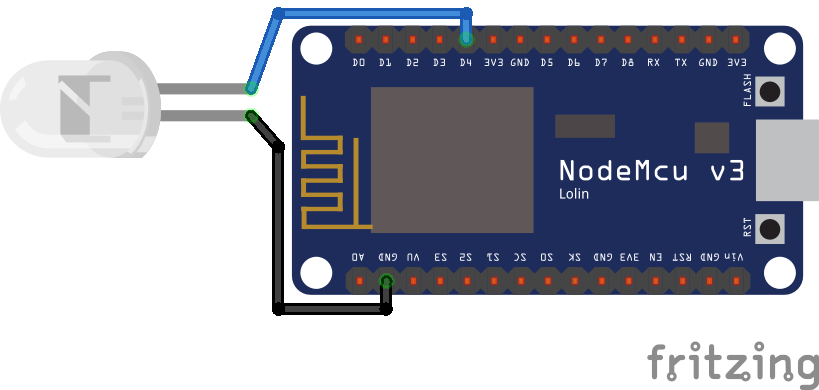
\includegraphics[height=2.5in]{figures/nodemcu-test1.png}
\caption[Montaje placa nodeMCU con led]{Esquema de montaje de led en una placa nodemcu}
    \label{figure1}
\end{figure}

A continuación debe compilarse el proyecto y subirse a la placa, una vez terminado el proceso, el led debe parpadear según lo programado:

\begin{verbatim}
    arduino-cli compile --fqbn esp8266:esp8266:nodemcuv2 test/test
    arduino-cli upload -p /dev/ttyUSB0 --fqbn esp8266:esp8266:nodemcuv2 test/test
\end{verbatim}

Habiendo verificado el proceso de subida es necesario probar que la conexión inalámbrica y la comunicación mediante el protocolo \gls{mqtt} es correcta, con un código distinto. Instanciar un nuevo proyecto, incluir el código, subir el sketch en la placa y probar la comunicación de la placa con el servidor. Es necesario además agregar las librerías necesarias, en el caso que ocupa este proyecto se utiliza la librería PubSubClient de Nick O'Leary, un cliente ligero de MQTT que posee buena estabilidad y facil integración en código.

\begin{verbatim}
    cd ~/Arduino
    arduino-cli lib search PubSubClient
    arduino-cli lib install "PubSubClient"
    arduino-cli sketch new testmqtt
    nano test/testmqtt.ino
\end{verbatim}

El código de prueba de \gls{mqtt} incluye la librería de ESP8266WiFi.h que no es necesario añadir mediante el instalador de librerías, ya que este viene incluido en el core de tarjetas de terceros que se incluyo anteriormente para el chip esp8266. De esta forma, el código incluye los parámetros de conexión \gls{wifi} para el adaptador de red inalámbrico del nodo principal y la conexión al servicio de \gls{mqtt} así como la publicación de topics. El siguiente, es un ejemplo básico para hacer pruebas es una ligera modificación del ejemplo contenido en la ruta \path{~/Arduino/libraries/PubSubClient/examples/mqtt_basic/mqtt_basic.ino}.


\begin{verbatim}
#include <ESP8266WiFi.h>
#include <PubSubClient.h>

const char* ssid = "edomus";
const char* password = "sistemaguardian1970.";
const char* mqtt_server = "192.168.4.1";

WiFiClient espClient;
PubSubClient client(espClient);
char msg[50];
long lastMsg = 0;
int value = 0;

 
void setup_wifi() {
  delay(10);
  // We start by connecting to a WiFi network
  WiFi.begin(ssid, password);
  while (WiFi.status() != WL_CONNECTED) {
    delay(500);
  }
  randomSeed(micros());
}
 
void callback(char* topic, byte* payload, unsigned int length) {
  // Switch on the LED if an 1 was received as first character
  if ((char)payload[0] == '1') {
    digitalWrite(BUILTIN_LED, LOW);   // Turn the LED on (Note that LOW is the voltage level
    // but actually the LED is on; this is because
    // it is acive low on the ESP-01)
  } else {
    digitalWrite(BUILTIN_LED, HIGH);  // Turn the LED off by making the voltage HIGH
  }
}
 
void reconnect() {
  // Loop until we're reconnected
  while (!client.connected()) {
    // Create a random client ID
    String clientId = "nodemcuClient-test";
    clientId += String(random(0xffff), HEX);
    
    // Attempt to connect
    if (client.connect(clientId.c_str())) {
      client.publish("outTopic", "hello world");
      client.subscribe("*/test");
    } else {
      delay(5000);
    }
  }
}

void setup() {
  pinMode(BUILTIN_LED, OUTPUT);     // Initialize the BUILTIN_LED pin as an output
  setup_wifi();
  client.setServer(mqtt_server, 1883);
  client.setCallback(callback);
}
 
void loop() {
  if (!client.connected()) {
    reconnect();
  }
  client.loop();
  long now = millis();
  
  if (now - lastMsg > 2500) {
    lastMsg = now; 
    ++value;
    snprintf (msg, 50, "hello world #%ld", value);
    client.publish("test/msg", msg);
  }
}
\end{verbatim}

Una vez subido el sketch a la placa según los pasos anteriormente indicados, podemos realizar una llamada a la placa mediante el cliente de \gls{mqtt} instalado en el nodo principal. El cual generara una salida de texto sin fin. Con esto, queda probado que el proceso de subida y la placa están en condiciones óptimas de funcionamiento.

\begin{verbatim}
    mosquitto_sub -h localhost -t test/msg
\end{verbatim}

\section{Scritps de generación de sckets placas nodeMCU desde Raspberry Pi}
\label{AppendiA:Key5}

Crear un sketch mediante un script puede variar en su complejidad en el grado de cuantos argumentos reciba y que tan flexible se desea que sea su comportamiento. Sea cual sea el tipo de sketch que se busque crear, se debe mantener una estructura de carga de librerías y constantes, un constructor y un bucle de ejecución. Considerando las necesidades del proyecto, se requiere que el script reciba los siguientes argumentos de entrada:

\begin{itemize}
  \item Modelo de la placa microcontroladora en la que se sube el sketch.

  \item Modelo del sensor/actuador que va a conectarse en el GPIO de la placa microcontroladora.

  \item Valor numérico del pin de conexión de I/O en el que se conectara el sensor/actuador.
  
  \item Nombre de la estancia en la que se planea ubicar la placa microcontroladora.
\end{itemize}

El objetivo ultimo del \gls{script} es generar un \gls{sketch} de Arduino que pueda compilarse correctamente, sin embargo, hasta que se reciben los argumentos solo es posible disponer de una plantilla genérica con secciones que deben ser rellenadas en base a las opciones. El modelo de plantilla básico puede constituirse con código previamente escrito en diferentes ficheros para luego ser ordenadamente ensamblada en un único fichero de código. En el caso de este proyecto se creara una estructura de carpetas constituida por un directorio principal, el script generador, un directorio con las secciones de código común a todos los sketchs y directorios separados para cada sensor/actuador disponible en la aplicación. Para la prueba inicial incluiremos el código del sensor DHT11 para un configurar una placa detectora de temperatura y humedad. En términos generales, un sensor/actuador requiere de 3 bloques de código que integrar en código común, las librerías y constantes, la configuración inicial del setup, y el código del bucle que sera requerido por el protocolo \gls{mqtt} para responder al servidor.

\begin{verbatim}
    cd ~
    mkdir sketchgenerator
    touch sketchgenerator/sketchgenerator
    mkdir sketchgenerator/general
    touch sketchgenerator/general/loop
    touch sketchgenerator/general/setup
    mkdir sketchgenerator/dht
    touch sketchgenerator/dht/dht11Lib
    touch sketchgenerator/dht/dht11Loop
    touch sketchgenerator/dht/dht11Setup
\end{verbatim}

Con esta estructura, el \gls{script} tendra que construir un ficehro de extensión .ino válido en la ruta de destino necesaria para que posteriormente arduino-cli pueda compilarlo y subirlo a la placa microcontroladora conectada a un puerto USB del nodo principal. Primero consideraremos el codigo de uso comun a todos los \gls{sketch}.

\begin{verbatim}
    nano sketchgenerator/general/setup
\end{verbatim}

Considerando que el sensor DHT11 posee cierto código que se incluye en la función setup, se usara una cadena de caracteres a modo de centinela, el cual sera sustituido por el código definido en un fichero concreto (dht11Setup, en este caso) situado en el directorio del sensor definido por los argumentos del srcipt generador. Dicho centinela en este codigo aparece como \verb|SETUP_THING|.

\begin{verbatim}
long lastMsg = 0;
char msg[50];
int value = 0;

void setup() {
  pinMode(BUILTIN_LED, OUTPUT);
  setup_wifi();
  client.setServer(mqtt_server, 1883);
  client.setCallback(callback);

  SETUP_THING
}

void setup_wifi() {
  delay(10);
  WiFi.begin(ssid, password);
  while (WiFi.status() != WL_CONNECTED) {
    delay(500);
  }
}

void callback(char* topic, byte* payload, unsigned int length) {
  if ((char)payload[0] == '1') {
    digitalWrite(BUILTIN_LED, LOW);
  } else {
    digitalWrite(BUILTIN_LED, HIGH);
  }
}

void reconnect() {
  while (!client.connected()) {
    if (client.connect("ESP8266Client")) {
      client.publish("outTopic", "hello world");
      client.subscribe("inTopic");
    } else {
      delay(5000);
    }
  }
}
\end{verbatim}

El siguiente segmento de código común corresponde al bucle sin fin de un \gls{sketch}. Al igual que en el caso anterior, una sección del código deberá ser rellenada por las particularidades del sensor. Para este caso se ha definido un centinela \verb|MAIN_BODY|.

\begin{verbatim}
    nano sketchgenerator/general/loop
\end{verbatim}

\begin{verbatim}
void loop() {
if (!client.connected()) {
    reconnect();
  }
  client.loop();
  long now = millis();
  if (now - lastMsg > 2500) {
    lastMsg = now;
    MAIN_BODY
  }
}
\end{verbatim}

Para las secciones de código de un sensor como el DHT se requiere de las librerías, funciones auxiliares y constantes propias.
\begin{verbatim}
    nano sketchgenerator/dht/dht11Lib
\end{verbatim}

\begin{verbatim}
#include <Adafruit_Sensor.h>
#include <DHT.h>
#include <DHT_U.h>
#define DHTPIN ARGUMENT_PIN
#define DHTTYPE DHT11
DHT dht(DHTPIN, DHTTYPE);
\end{verbatim}

Tambien es necesario el segmento de codigo que se incluye en la fución setup.
\begin{verbatim}
    nano sketchgenerator/dht/dht11Lib
\end{verbatim}

\begin{verbatim}
dht.begin();
\end{verbatim}

Y por ultimo el segmento de código que sera invocado en la función loop que incluye la respuesta del cliente \gls{mqtt}. Este segmento de código también incluye centinelas que deben ser sustituidos en base a los argumentos del generador de \gls{sketch}, ya que de otra forma no seria posible definir los topics a los que responderá la placa cuando el nodo solicite información.
\begin{verbatim}
    nano sketchgenerator/dht/dht11Lib
\end{verbatim}

\begin{verbatim}
float h = dht.readHumidity();
float t = dht.readTemperature();
if (isnan(h) || isnan(t))
{
    snprintf (msg, 75, "{'status':'error', 'message':'Error in DHT11 sensor'}", value);
    client.publish("nodemcudht11", msg);
}
else
{
    snprintf (msg, 75, "'%f'", t);
    client.publish("TOPIC_PLACA/temp", msg);
    snprintf (msg, 75, "'%f'", h);
    client.publish("TOPIC_PLACA/hum", msg);
}
\end{verbatim}

Con todo este código por segmentado puede constituirse un \gls{sketch} valido siempre que se encadene en el orden correcto con las sustituciones adecuadas. El script se ejecutara en el entorno de \verb|Bash|, y realizara la recepción de los argumentos, validación de los mismos y verificación de las rutas de los ficheros de donde se obtendrán los segmentos de codigo de cada parte. Serán unidos y escritos en un fichero situado en la ruta de un proyecto de Arduino que actuara como contenedor para las compilaciones. El srcipt ademas dispone de los credenciales necesarios para la conexión \gls{wifi} al nodo y el servicio de \gls{mqtt}.

\begin{verbatim}
    nano sketchgenerator/sketchgenerator
\end{verbatim}

\begin{verbatim}
#!/bin/bash

destinyPath=../sketchbook/nodemcu.ino

BASICLIBRARIES="#include <ESP8266WiFi.h>\n#include <PubSubClient.h>"

echo -e $BASICLIBRARIES "\n\n"> $destinyPath

#$1 path to sensor
#$2 pint for I/O in sensor
[ $# -eq 0 ] && { echo "Usage: $1 sensor path"; exit 1; }
[ ! -f "$1" ] && { echo "Error: $1 file not found."; exit 2; }
file=$1
pin="D$2"
#Si fichero existe y no es vacio
if [ -s $file ]
then
        while IFS= read -r line
        do
        replace="${line/ARGUMENT_PIN/$pin}"
        echo -e $replace >> $destinyPath
        done < "$file"
else
        echo -e "FICHERO SOLICITADO NO EXISTE\n"
        exit
fi

ACCESS_POINT="const char* ssid = \"edomus\";\n"
PASSWORD="const char* password = \"sistemaguardian1970.\";\n"
MQTT_SERVER="const char* mqtt_server = \"192.168.4.1\";\n"
WIFI_CONST="WiFiClient espClient;\n"
WIFI_CLI="PubSubClient client(espClient);\n"


echo -e $ACCESS_POINT$PASSWORD$MQTT_SERVER$WIFI_CONST$WIFI_CLI >> $destinyPath



#GET SETUP FOR SELECTED THING
thingSetup=""
[ ! -f "$1Setup" ] && { echo "Error: $1Setup file not found."; exit 2; }
if [ -s "$1Setup" ]
then
        while IFS= read -r line
        do
        thingSetup+=$line
        done < "$1Setup"
fi

[ ! -f "general/setup" ] && { echo "Error: setup file not found."; exit 2; }
if [ -s "general/setup" ]
then
        while IFS= read -r line
        do
        main="${line/SETUP_THING/$thingSetup}"
        echo -e $main >> $destinyPath
        done < "general/setup"
fi
\end{verbatim}
% +--------------------------------------------------------------------+
% | Appendix B Page (Optional)                                         |
% +--------------------------------------------------------------------+

\cleardoublepage

\chapter{Troubleshooting}
\label{AppendiB:Key1}

\section{Proceso de subida de sckets pacas nodeMCU desde Raspberry Pi}
\label{AppendiB:Key2}

sudo apt-get install git raspberrypi-kernel-headers build-essential dkms
https://github.com/juliagoda/CH341SER
nano328


\section{Error en la instlación de mosquitto}
\label{AppendiB:Key3}
-- Error

The following packages have unmet dependencies:
 mosquitto : Depends: libssl1.0.0 (>= 1.0.0) but it is not installable
             Depends: libwebsockets3 (>= 1.2) but it is not installable

--- solucion
https://theembeddedlab.com/tutorials/install-mosquitto-on-a-raspberry-pi/

% +--------------------------------------------------------------------+
% | Enter text for your Appendix page in the space below this box.     |
% |                                                                    |
% +--------------------------------------------------------------------+

\section{Margenes de error del sensor DHT11}
\label{AppendiB:key4}
sensor DHT version 1.4. Se debe realizar una prueba de contacto con un script que nos muestre la información por pantalla para verificar que las conexiones del sensor a la rapsberry son correctos. Este primer script es un bucle infinito de mediciones de temperatura y humedad cada poco segundos. Hay una justificación para elegir un bucle sobre una única medida del sensor y está fundamentada en el margen de error inicial de las medidas. Si bien el sensor DTH11 es una opción muy común por su bajo coste y facilidad de implementación (este sensor se caracteriza por tener la señal digital calibrada por lo que asegura una alta calidad y una fiabilidad a lo largo del tiempo, ya que contiene un microcontrolador de 8 bits integrado. Está constituido por dos sensores resistivos (NTC y humedad) - revisar esta info y contrastarla contra ésta: \url{https://programarfacil.com/blog/arduino-blog/sensor-dht11-temperatura-humedad-arduino/} ), ademas de manejar señales digitales que no se ven afectadas por las fluctuaciones de voltaje, tiene algunas contrapartidas que deben tenerse en cuenta. Se necesita un tiempo mínimo de espera entre medidas (de al menos 1 segundo), hecho que no agrava particularmente su desempeño en entornos cerrados como una casa, ya que las variaciones de temperatura y humedad no son bruscas, aun así existen estrategias para reducir estos tiempos, por ejemplo, usar la función millis() de Arduino, el cual nos da el tiempo en milisegundos desde que empieza a ejecutarse el código, De esta forma evitamos la pausa de los 2 segundos, pero no el tiempo que demora en hacer la lectura, que es de aproximadamente  250 milisegundos, el cual lo pueden notar si realizan el ejemplo anterior, en donde se hace parpadear el led interno de la placa (Pin 13) con pausas de 100ms (tomado de \url{https://naylampmechatronics.com/blog/40_Tutorial-sensor-de-temperatura-y-humedad-DHT1.html}). Otro problema que abordar es que las primeras lecturas tienen un margen de error de unos +-2 grados Celsius y +-5\% de humedad relativa en las primeras 4 lecturas. Esto generará un problema a la hora de tomar lecturas instantáneas si el sensor no se encuentra ya operando cuando se solicita el dato.
% +--------------------------------------------------------------------+
% | Appendix B Page (Optional)                                         |
% +--------------------------------------------------------------------+

\cleardoublepage

\chapter{Diagramas}
\label{AppendiC:Key1}

\begin{figure}[hbt!]
\centering
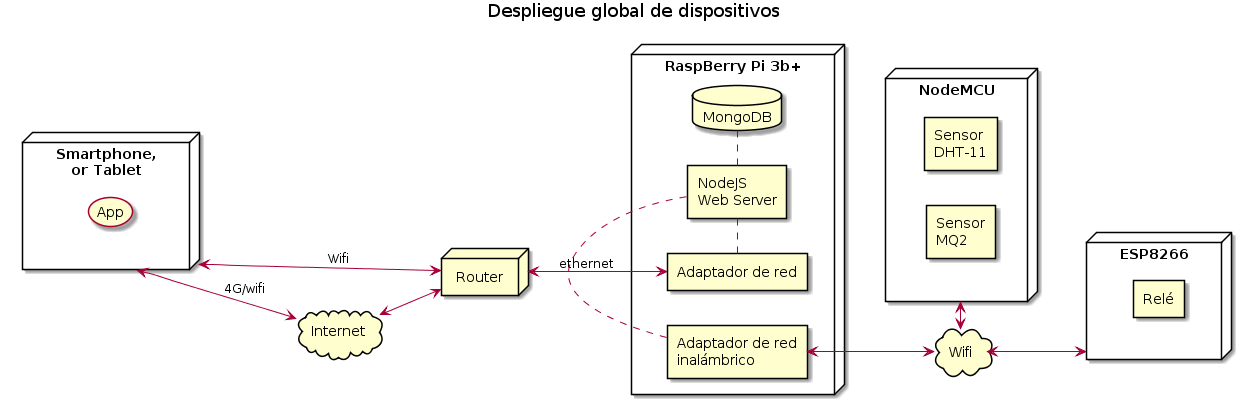
\includegraphics[height=2.4in]{figures/diagrams/physical-devices/global.png}
\caption[Diagrama de despiegue de dispositivos]{Diagrama de despliegue de dispositivos\footnotemark}
\end{figure}

% +--------------------------------------------------------------------+
% | Enter text for your Appendix page in the space below this box.     |
% |                                                                    |
% +--------------------------------------------------------------------+


\clearpage
 
\printglossary[type=\acronymtype, title=Acrónimos, toctitle=Lista de acrónimos, style=long]

\end{document}
